%%%%%%%%%%%%%%%%%%%%%%%%%%%%%%%%%%%%%%%%%
% Masters/Doctoral Thesis
% LaTeX Template
% Version 1.43 (17/5/14)
%
% This template has been downloaded from:
% http://www.LaTeXTemplates.com
%
% Original authors:
% Steven Gunn
% http://users.ecs.soton.ac.uk/srg/softwaretools/document/templates/
% and
% Sunil Patel
% http://www.sunilpatel.co.uk/thesis-template/
%
% License:
% CC BY-NC-SA 3.0 (http://creativecommons.org/licenses/by-nc-sa/3.0/)
%
% Note:
% Make sure to edit document variables in the Thesis.cls file
%
%%%%%%%%%%%%%%%%%%%%%%%%%%%%%%%%%%%%%%%%%

%----------------------------------------------------------------------------------------
%	PACKAGES AND OTHER DOCUMENT CONFIGURATIONS
%----------------------------------------------------------------------------------------

\documentclass[11pt, oneside]{Thesis} % The default font size and one-sided printing (no margin offsets)

\graphicspath{{Pictures/}} % Specifies the directory where pictures are stored
\usepackage[x11names,table]{xcolor}
\usepackage[utf8]{inputenc}
\usepackage[T1]{fontenc}
\usepackage{lmodern}
\usepackage{textcomp}
\usepackage{dsfont}
\usepackage{subfig}
\usepackage[spanish]{babel}
\usepackage{float}
\usepackage{acronym}
\usepackage{comment}
\usepackage{csquotes}
\usepackage{multirow}
\usepackage{minted}
\usepackage[titletoc]{appendix}
\usepackage[colorinlistoftodos,prependcaption,textsize=tiny]{todonotes}
\usepackage[square, numbers, comma, sort&compress]{natbib} % Use the natbib reference package - read up on this to edit the reference style; if you want text (e.g. Smith et al., 2012) for the in-text references (instead of numbers), remove 'numbers'
\hypersetup{urlcolor=blue, colorlinks=true} % Colors hyperlinks in blue - change to black if annoying
\title{\ttitle} % Defines the thesis title - don't touch this
\setlength{\parindent}{12pt}
\begin{document}

\frontmatter % Use roman page numbering style (i, ii, iii, iv...) for the pre-content pages

\setstretch{1.3} % Line spacing of 1.3

% Define the page headers using the FancyHdr package and set up for one-sided printing
\fancyhead{} % Clears all page headers and footers
\rhead{\thepage} % Sets the right side header to show the page number
\lhead{} % Clears the left side page header

\pagestyle{fancy} % Finally, use the "fancy" page style to implement the FancyHdr headers

\newcommand{\HRule}{\rule{\linewidth}{0.5mm}} % New command to make the lines in the title page

% PDF meta-data
\hypersetup{pdftitle={\ttitle}}
\hypersetup{pdfsubject=\subjectname}
\hypersetup{pdfauthor=\authornames}
\hypersetup{pdfkeywords=\keywordnames}

%----------------------------------------------------------------------------------------
%	TITLE PAGE
%----------------------------------------------------------------------------------------

\begin{titlepage}
\begin{center}

\textsc{\LARGE Facultad de Ingeniería \\ Universidad de Buenos Aires}\\[1.5cm] % University name
\textsc{\Large TESIS DE INGENIERÍA INFORMÁTICA}\\[0.5cm] % Thesis type

\HRule \\[0.4cm] % Horizontal line
{\huge \bfseries Diseño y calibración de una antena polarimétrica por acoplamientos mutuos}\\[0.4cm] % Thesis title
\HRule \\[1.5cm] % Horizontal line

\begin{minipage}{0.4\textwidth}
\begin{flushleft} \large
\emph{Autor:}\\
{José Francisco Soler} % Author name - remove the \href bracket to remove the link
\end{flushleft}
\end{minipage}
\begin{minipage}{0.4\textwidth}
\begin{flushright} \large
\emph{Directora:} \\
{Lic. Rosa Wachenchauzer} \\
\emph{Co Director:} \\
{Ing. Pablo Marino} % Supervisor name - remove the \href bracket to remove the link
\end{flushright}
\end{minipage}\\[3cm]

%\large \textit{A thesis submitted in fulfilment of the requirements\\ for the degree of \degreename}\\[0.3cm] % University requirement text
%\textit{in the}\\[0.4cm]
Departamento de informática\\
2016\\[2cm] % Research group name and department name

%{\large \today}\\[4cm] % Date

\includegraphics[width=4cm]{Logo2.png} % University/department logo - uncomment to place it

\vfill
\end{center}

\end{titlepage}

%----------------------------------------------------------------------------------------
%	DECLARATION PAGE
%	Your institution may give you a different text to place here
%----------------------------------------------------------------------------------------

% \Declaration{
%
% \addtocontents{toc}{\vspace{1em}} % Add a gap in the Contents, for aesthetics
%
% I, \authornames, declare that this thesis titled, '\ttitle' and the work presented in it are my own. I confirm that:
%
% \begin{itemize}
% \item[\tiny{$\blacksquare$}] This work was done wholly or mainly while in candidature for a research degree at this University.
% \item[\tiny{$\blacksquare$}] Where any part of this thesis has previously been submitted for a degree or any other qualification at this University or any other institution, this has been clearly stated.
% \item[\tiny{$\blacksquare$}] Where I have consulted the published work of others, this is always clearly attributed.
% \item[\tiny{$\blacksquare$}] Where I have quoted from the work of others, the source is always given. With the exception of such quotations, this thesis is entirely my own work.
% \item[\tiny{$\blacksquare$}] I have acknowledged all main sources of help.
% \item[\tiny{$\blacksquare$}] Where the thesis is based on work done by myself jointly with others, I have made clear exactly what was done by others and what I have contributed myself.\\
% \end{itemize}
%
% Signed:\\
% \rule[1em]{25em}{0.5pt} % This prints a line for the signature
%
% Date:\\
% \rule[1em]{25em}{0.5pt} % This prints a line to write the date
% }
%
% \clearpage % Start a new page

%----------------------------------------------------------------------------------------
%	QUOTATION PAGE
%----------------------------------------------------------------------------------------

% \pagestyle{empty} % No headers or footers for the following pages
%
% \null\vfill % Add some space to move the quote down the page a bit
%
% \textit{``Thanks to my solid academic training, today I can write hundreds of words on virtually any topic without possessing a shred of information, which is how I got a good job in journalism."}
%
% \begin{flushright}
% Dave Barry
% \end{flushright}
%
% \vfill\vfill\vfill\vfill\vfill\vfill\null % Add some space at the bottom to position the quote just right
%
% \clearpage % Start a new page

%----------------------------------------------------------------------------------------
%	ABSTRACT PAGE
%----------------------------------------------------------------------------------------
%
\addtotoc{Resumen} % Add the "Abstract" page entry to the Contents

\abstract{\addtocontents{toc}{\vspace{1em}} % Add a gap in the Contents, for aesthetics

Las antenas en fase (del ingles: phased array) son un conjunto de antenas en el cual las fases relativas de las señales con que
se alimenta cada antena se varían intencionalmente con objeto de alterar el diagrama de radiación del conjunto. Lo normal es 
reforzar la radiación en una dirección concreta y suprimirla en direcciones indeseadas \cite{Standard1996}.

Un conjunto de antena es un ejemplo de difracción, dado que puede ser visto como la suma de N fuentes lineales y coherentes. 
Cada antena individual hace el papel de una abertura, emitiendo ondas de radio cuyo diagrama de difracción puede ser calculado 
sumando el desplazamiento de fase $\varphi$.

En la actualidad, los conjuntos de antenas de fase variable son ampliamente utilizados, por ejemplo, en estaciones de difusión
tanto AM como FM, para estudios climatológicos y en el uso de satélites y radares tanto para uso marítimo (barcos de guerra de
diversas armadas) como terrestres. La principal ventaja de este tipo de antenas con respecto a otras (isotópica, monopolos), es 
el hecho de poder realizar apuntamientos electrónicamente, es decir, que se pueden direccionar de manera electrónica sin tener 
que hacer uso de elementos mecánicos. Dichos elementos poseen ciertas desventajas asociadas tanto desde el punto de vista del 
mantenimiento como de velocidad de respuesta. 

Hay numerosos factores que modifican el comportamiento de la antena y por ende el apuntamiento, que es en esencia lo que se desea
tener bajo control, también de manera electrónica. Por ejemplo, cambios de temperatura o el mero envejecimiento de los elementos
que la componen, que lleva a que la respuesta final del sistema no sea la esperada. Es deseable tener dichos factores bajo control
y así poder apuntar en la dirección deseada. Para ello se hace uso de un esquema de calibración interna, el cual debe permitir
conocer con una determinada exactitud dicho apuntamiento.

Se investiga y presenta el esquema de calibración interna convencional con sus virtudes y sus defectos. Con dicha información
se introduce un método que complemente las falencias sin agregar elementos adicionales al sistema. 

En primer termino, se investigan y presentan las hipotesis necesarias para la aplicación de la calibración aquí propuesta. 
Esto significa por ejemplo pedir que el sistema sea lineal e invariante en el tiempo, que los niveles de acoplamiento entre 
elementos radiantes sea conocido, que el sistema disponga de determinados mecanismos de autoprotección, entre otros.

En segunda instancia, y basado en las hipótesis propuestas, se propone, diseña, y construye en software un modelo físico 
representativo ad hoc desde el punto de vista de radio frecuencia, que servirá de base para evaluar el modelo de calibración 
propuesto. Este modelo físico se realiza con ciertas premisas, como ser por ejemplo que sea flexible para evaluar diferentes 
topologías de antenas.

En tercera instancia se desarrollan ambos algoritmos de calibración y se los aplica a diferentes topologías de antena en fase 
para comparar los resultados obtenidos y así mostrar que el método propuesto supera ampliamente al clásico.

En última instancia, se plantean diferentes líneas futuras de trabajo.
}

\clearpage % Start a new page

%----------------------------------------------------------------------------------------
%	ACKNOWLEDGEMENTS
%----------------------------------------------------------------------------------------

\setstretch{1.3} % Reset the line-spacing to 1.3 for body text (if it has changed)

\acknowledgements{\addtocontents{toc}{\vspace{1em}} % Add a gap in the Contents, for aesthetics

Quiero agradecer enormemente a toda mi familia, quienes me apoyaron durante todos estos años. A mis hermanas, que me recibieron
en su casa durante tantos fines de semana y por sobre todas las personas a mis queridos padres. No tengo palabras para expresar
la enorme gratitud que tengo dado que nunca perdieron la fe en mi, siempre me apoyaron y siempre estuvieron ahí cuando los necesité.
También quiero agradecer a todos los amigos que fui haciendo durante los años facultativos y en especial a Leandro y Ezequiel,
quienes siempre me dieron palabras de aliento para los peores momentos. Y por último, quiero agradecer a Pablo, quien sin él 
este trabajo no hubiese sido posible.\ldots
}
\clearpage % Start a new page

%----------------------------------------------------------------------------------------
%	LIST OF CONTENTS/FIGURES/TABLES PAGES
%----------------------------------------------------------------------------------------

\pagestyle{fancy} % The page style headers have been "empty" all this time, now use the "fancy" headers as defined before to bring them back

\lhead{\emph{Contenidos}} % Set the left side page header to "Contents"
\tableofcontents % Write out the Table of Contents

\lhead{\emph{Lista de figuras}} % Set the left side page header to "List of Figures"
\listoffigures % Write out the List of Figures

\lhead{\emph{Lista de cuadros}} % Set the left side page header to "List of Tables"
\listoftables % Write out the List of Tables

%----------------------------------------------------------------------------------------
%	ABBREVIATIONS
%----------------------------------------------------------------------------------------

\clearpage % Start a new page

% \setstretch{1.5} % Set the line spacing to 1.5, this makes the following tables easier to read
%
% \lhead{\emph{Abbreviations}} % Set the left side page header to "Abbreviations"
% \listofsymbols{ll} % Include a list of Abbreviations (a table of two columns)
% {
% \textbf{LAH} & \textbf{L}ist \textbf{A}bbreviations \textbf{H}ere \\
% %\textbf{Acronym} & \textbf{W}hat (it) \textbf{S}tands \textbf{F}or \\
% }
\lhead{\emph{Acrónimos}}
\chapter*{Acrónimos}

\begin{acronym}[UML]
	\acro{AM}{Amplitud Modulada}
	\acro{FM}{Frecuencia Modulada}
\acro{RF}{Radio Frequency}
\acro{PRF}{Frecuencia de repetición del pulso (del inglés)}

\acro{CE}{Electrónica Central (del inglés)}
\acro{RFDN}{Red de distribución de RF (del inglés)}
\acro{PSC}{Divisor/combinador de potencia de RF (del inglés)}
\acro{TRM}{Módulo de transmisión/recepción (del inglés)}
\acro{TR}{transmisión/recepción}
\acro{RM}{Módulo radiante (del inglés)}
\acro{ER}{Elemento radiante}
\acro{LTI}{Lineal e invariante en el tiempo (del inglés)}

\acro{SAR}{Radar de apertura sintética (del inglés)}

\acro{PA}{Conjunto de antenas controladas en fase (del inglés)}
\acro{LCI}{Lazo de calibración interna}
\acro{VHF}{Muy alta frecuencia (del inglés)}
\acro{UHF}{Ultra alta frecuencia (del inglés)}

\acro{VNA}{Analizador de redes vectorial (del inglés)}
\acro{SWR}{Relación de onda estacionaria (del inglés)}
\acro{ROE}{Relación de onda estacionaria}

\acro{E-ERS}{Relación de onda estacionaria}
\acro{SIR-C}{Relación de onda estacionaria}
\end{acronym}
%----------------------------------------------------------------------------------------
%	PHYSICAL CONSTANTS/OTHER DEFINITIONS
%----------------------------------------------------------------------------------------

% \clearpage % Start a new page
%
% \lhead{\emph{Physical Constants}} % Set the left side page header to "Physical Constants"
%
% \listofconstants{lrcl} % Include a list of Physical Constants (a four column table)
% {
% Speed of Light & $c$ & $=$ & $2.997\ 924\ 58\times10^{8}\ \mbox{ms}^{-\mbox{s}}$ (exact)\\
% % Constant Name & Symbol & = & Constant Value (with units) \\
% }

%----------------------------------------------------------------------------------------
%	SYMBOLS
%----------------------------------------------------------------------------------------

% \clearpage % Start a new page
%
% \lhead{\emph{Symbols}} % Set the left side page header to "Symbols"
%
% \listofnomenclature{lll} % Include a list of Symbols (a three column table)
% {
% $a$ & distance & m \\
% $P$ & power & W (Js$^{-1}$) \\
% % Symbol & Name & Unit \\
%
% & & \\ % Gap to separate the Roman symbols from the Greek
%
% $\omega$ & angular frequency & rads$^{-1}$ \\
% % Symbol & Name & Unit \\
% }

%----------------------------------------------------------------------------------------
%	DEDICATION
%----------------------------------------------------------------------------------------

% \setstretch{1.3} % Return the line spacing back to 1.3
%
% \pagestyle{empty} % Page style needs to be empty for this page
%
% \dedicatory{For/Dedicated to/To my\ldots} % Dedication text
%
% \addtocontents{toc}{\vspace{2em}} % Add a gap in the Contents, for aesthetics

%----------------------------------------------------------------------------------------
%	THESIS CONTENT - CHAPTERS
%----------------------------------------------------------------------------------------

\mainmatter % Begin numeric (1,2,3...) page numbering

\pagestyle{fancy} % Return the page headers back to the "fancy" style

% Include the chapters of the thesis as separate files from the Chapters folder
% Uncomment the lines as you write the chapters

% Chapter 1

\chapter{Introducción} % Chapter title

\label{ch:introduccion} % For referencing the chapter elsewhere, use \autoref{ch:introduccion} 
\lhead{\emph{Introducción}} % Change X to a consecutive number; this is for the header on each page - perhaps a shortened title

%----------------------------------------------------------------------------------------
En este capítulo se dará una breve introducción a la problemática a resolver. Las siguientes secciones tratarán la motivación,
la definición del problema a trabajar y el plan de tesis.

\section{Definiciones}

{\textbf{Antena:}} Es un objeto eléctrico el cual convierte potencia eléctrica en ondas de radio y viceversa. Usualmente es 
utilizada con un transmisor o receptor de radio. En transmisión, el transmisor provee una corriente eléctrica oscilando en 
RF en los terminales de la antena, y la antena radía dicha energía como ondas electromagnéticas (ondas de radio). En 
recepción, una antena intercepta parte de la onda electromagnética en orden de producir una mínima tensión en sus terminales,
que es aplicado al receptor a ser amplificado \cite{AntennaWiki}.

{\textbf{Polarización:}} La polarización de una antena hace referencia a la orientación del campo eléctrico (plano-E) de la 
onda de radio con respecto a la superficie terrestre y es determiada por la estructura física de la antena y por su 
orientación. Por lo tanto, una antena que sea simplemente un cable recto poseerá una polarización cuando se la monta 
verticalmente, y otra diferente cuando sea horizontalmente. Como una onda transversal, el campo magnético de una onda de 
radio es perpendicular al eléctrico, pero, por convención, la polarización hace referencia a la dirección del campo 
eléctrico \cite{AntennaWiki}.

\todo{agregar ROE y SWR como definición}

{\textbf{Adaptación de impedancias:}} La máxima transferencia de potencia requiere que la impedancia de un sistema de 
antena esté adaptada al conjugado complejo de la impedancia del transmisor o receptor. En el caso de un transmisor, 
la impedancia adaptada deseada no necesariamente corresponde a la impedancia de salida dinámica del transmisor analizado
como una fuente de impedancia sino al valor de diseño (típicamente de $50 \Omega$) requerido para una operación eficiente
y segura del circuito de transmisión. Normalmente, la impedancia deseada es resistiva pero un transmisor (y algunos receptores)
pueden tener ajustes adicionales para cancelar una cierta cantidad de reactancia en orden de obtener dicha adaptación. Cuando
una linea de transmisión es usada entre la antena y el transmisor (o receptor) uno generalmente desearía un sistema de antena
con una impedancia resistiva y cercana a la impedancia característica de dicha línea de transmisión, para minimizar el SWR \todo{buscar que es el swl}
e incrementar la transmisión \cite{AntennaWiki}. 


Maximum power transfer requires matching the impedance of an antenna system (as seen looking into the transmission line) to the complex conjugate of the impedance of the receiver or transmitter. In the case of a transmitter, however, the desired matching impedance might not correspond to the dynamic output impedance of the transmitter as analyzed as a source impedance but rather the design value (typically 50 ohms) required for efficient and safe operation of the transmitting circuitry. The intended impedance is normally resistive but a transmitter (and some receivers) may have additional adjustments to cancel a certain amount of reactance in order to "tweak" the match. When a transmission line is used in between the antenna and the transmitter (or receiver) one generally would like an antenna system whose impedance is resistive and near the characteristic impedance of that transmission line in order to minimize the standing wave ratio (SWR) and the increase in transmission line losses it entails, in addition to supplying a good match at the transmitter or receiver itself.



{\textbf{Antena de arreglo de fase:}} \todo{poner referencias en esta definicion} (en inglés: phased array) es un conjunto de antenas en que las fases relativas de las 
señales con que se alimenta cada antena se varían intencionadamente con objeto de alterar el diagrama de radiación del 
conjunto. Lo normal es reforzar la radiación en una dirección concreta y suprimirla en direcciones indeseadas. Si todos los 
elementos del arreglo de fase están contenidos en el mismo plano y la señal con que se alimentan es de la misma fase, 
entonces se estará reforzando la dirección perpendicular a ese plano. Si se altera la fase relativa de las señales se podrá
\enquote*{mover} el haz (en realidad lo que se está haciendo es cambiar la dirección en la cual las interferencias son 
constructivas). Se consigue de este modo hacer barridos sin necesidad de movimiento físico, con la ventaja añadida de que 
se pueden barrer ángulos del orden de miles de grados por segundo. Esto permite utilizar la antena para compaginar 
simultáneamente funciones de detección y de seguimiento muchos blancos individuales, asi como para obtener imágenes de 
apertura sintética. Su uso se va extendiendo debido a la confiabilidad derivada del hecho de que no tienen partes móviles. 
Casi todos los radares militares modernos se basan en phased arrays, relegando los sistemas basados en antenas rotatorias a 
aplicaciones donde el costo es un factor determinante (tráfico aéreo, meteorología, etc) Su uso está también extendido en
aeronaves militares debido a su capacidad de seguir múltiples objetivos. El primer avión en usar uno fue el B-1B Lancer, y 
el primer caza, el MiG-31 ruso.\\

{\textbf{Calibración:}} Operación que, bajo determinadas condiciones, en un primer paso, establece una relación entre 
valores cuantitativos con incertidumbres de medición provistas por estandares de medición e indicaciones correspondientes
con incertidumbres asociadas (del instrumento calibrado o estandar secundario) y, en un segundo paso, usa
esta información para establecer una relación para obtener un resultado de una medición desde una indicación \cite{CalDef}.

{\textbf{Calibración interna:}} Las mediciones obtenidas utilizando este sistema son útiles solamente al utilizarlas en 
conjuto a los resultados de los test realizados en tierra, los cuales definen la relación entre lo observado y la 
performance de los párametros del sistema. Ejemplos de satélites para los cuales se utilizó calibración interna son el 
E-ERS-1 y el SIR-C.

Los tests realizados en tierra para dichos sistemas complejos son sobre la electrónica de RF, la electrónica digital y la 
antena sobre temperatura; para los cuales es preferible realizarlos, cuando sea posible, en un ambiente al vacío. Los 
parámetros clave del sistema, como: potencia transmitida, pérdidas de transmisión o recepción, ganancia de recepción, 
ganancia y patrón de la antena, linealidad de la electrónica digital/RF, rango dinámico, y fase/amplitud vs estabilidad de la 
frecuencia son medidos en función de la temperatura para cada seteo de ganancia del radar y PRF (Pulse Repetition Frequency). 
Los elementos de calibración, como medidores de temperatura, de corriente y de potencia, podrán permitir la determinación de 
la performance del sistema en función de la variación de dichos parámetros.
    
Esta técnica asume que la variación en la performance del sistema puede ser modelada en función de los parámetros observables. 
También, se asume que los componentes de calibración están correctamente calibrados y son estables en el paso del tiempo. 
Además de estos tests, en la mayoría de los sistemas de radar se realizan mediciones de componentes de RF utilizando lazos de 
calibración \cite{Curlander1991}.

{\textbf{Caracterización:}} significa medir (el desempeño de) los parámetros de la antena con el objeto de describir en 
forma comprensible su comportamiento \cite{Mittermayer2007}.

{\textbf{Caracterización del sistema:}} adicionalmente incluye la determinación de las curvas de características basadas 
en los modelos y en las mediciones indirectas de los parámetros, en el caso en que los parámetros no pueden ser medidos 
en forma directa \cite{Mittermayer2007}.

{\textbf{Calibración:}} significa el ajuste de la representación de los parámetros físicos en los productos que arroje la 
antena de manera que los mismos puedan ser medidos dentro la especificación \cite{Mittermayer2007}.

{\textbf{Verificación:}} significa mostrar mediante mediciones apropiadas que un sistema o subsistema trabaja dentro de su 
especificación (o conjunto de especificaciones) o que un producto cumple con su especificación \cite{Mittermayer2007}.


{\textbf{Campaña de caracterización:}}

\section{Contexto}

Una antena es un transductor que transforma la energía eléctrica en electromagnética 
en forma de ondas de radio transmitida en el aire o en el medio en que está la antena. A su vez, también sirve como 
receptor de dichas señales del medio. Hay una amplia variedad de antenas en la actualidad, los principales grupos y usos 
se los presentan en la tabla \ref{tab:type_antennas}.

\begin{table}[H]
  \footnotesize
  \centering
  \begin{tabular}{|c|p{9cm}|}
	\hline
	\textbf{Tipo Antena} & \textbf{Características} \\\hline
	Isotrópica & Es una antena hipotética, la cual radía la misma potencia en todas las direcciones.\\\hline
	Monopolo & Es un único módulo radiante, generalmente un simple cilindro de metal conectado en una punta a un plano de 
	tierra y en la otra a la línea de alimentación. Usos: Radio AM/FM, walkie talkie, etc. \\\hline
	Dipolo & Es el tipo de antena más comunmente utilizado, consiste en dos RMs simétricos, los cuales son cilindros 
	metálicos o cables. Usos: antena de canales de tv VHF, antena de televisión analógica, etc. \\\hline
	Arreglo & Consiste en múltiples antenas trabajando como una única antena. Usos: Transmisión de canales de tv en VHF, 
	detección de misiles, comunicaciones satelitales, etc.\\\hline
	Loop & Consiste en una o múltiples vueltas de cable. Trabajan con campos magnéticos en vez de eléctricos. Usos: receptora 
	de canales UHF de tv, receptoras de radio de Amplitud Modulada, etc.\\\hline
	Apertura & Son el principal tipo de antenas direccionales utilizadas en frecuencias microondas. Consisten en una antena 
	del tipo dipolo o Loop junto a una estructura que guía las ondas en una dirección determinada. Usos: Comunicaciones 
	satelitales, comunicaciones marinas, etc.\\\hline
  \end{tabular}
  \caption{Cacacterísticas de cada grupo principal de antenas}
  \label{tab:type_antennas}
\end{table}

La presente tesis se enfoca en el tipo arreglo de antena de fase contorlada, en particular sobre su calibración. Otras aplicaciones para 
las cuales son utilizadas es en comunicaciones móviles \cite{Chen2012}, aéreas \todo{encontrar la siguiente cita entre las cosas del mendeley}
[\ref{ppr:punc-ext1}] y espaciales \cite{Shimada1995}\cite{Makhoul2012}. 

Para generar diversos productos, por ejemplo imágenes satelitales en radares SAR \todo{encontrar la siguiente cita entre las cosas del mendeley}
[\ref{ppr:puncTrgt1}], es necesario que estén 
correctamente calibradas \todo{encontrar la siguiente cita entre las cosas del mendeley}
[\ref{ppr:classic1}]\cite{Seifert1996}\cite{Dall1994}. Esto implica, que las tolerancias de
fases y amplitudes se mantengan en el tiempo y/o sus valores sean bien conocidas
para cada elemento del arreglo.

Generalmente, este tipo de antenas son calibradas en tierra utilizando fuentes 
externas de campo lejano o cercano [\ref{ppr:mutual1}]. Sin embargo, en 
aplicaciones aéreas o espaciales, la utilización de dichas fuentes es impráctica
o difícil de implementar \cite{Aumann1989}. Resulta fundamental un esquema de
calibración interna que permita tener bajo control estas variables. 

Como consideración a la problemática que ninguno de los métodos a ser presentados de calibración interna pueden determinar
la potencia absoluta de transmisión de la antena como elemento único, se introducen los dos principales métodos de 
calibración externa para complementar esta falencia. 

Calibración utilizando blancos puntuales: Los blancos puntuales son dispositivos construidos por el hombre, generalmente son
corner reflectors, transponders, generadores de tono o receptores. La característica de estos dispositivos es que no solo 
son muy chicos con respecto a la mínia área de observación de una antena y que el eco de la señal de dichos dispositivos 
posee mucha más intensidad que dicha área, sino que el reflejo es bien conocido. Por lo tanto, con su uso se puede deducir la potencia transmitida.

Calibración utilizando blancos distribuidos: Se refiere a la utilización de blancos naturales de largas áreas con 
propiedades de backscattering homogéneas. Se utiliza la suposición que estas propiedades son estables o que su variación es 
bien conocida.

Una vez introducidos los métodos de calibración externa, se procede a explicar los de calibración interna.

El primer método a mencionar es el llamado método REV, el cual calibra de a un módulo radiante a la vez utilizando una 
antena externa al panel como receptora. El proceso de calibración es el siguiente, se transmite por un módulo radiante
y se va variando la fase hasta obtener la máxima potencia recibida, luego se repite el proceso para todos los módulos. 

Otro método es el convencional, el cual implementa lazos internos de para calibrar los caminos de transmisión y 
recepción de la antena de forma independiente [\ref{ppr:classic1}]\cite{Seifert1996}\cite{Dall1994}\cite{Freeman1995}
[\ref{ppr:classic4}][\ref{ppr:classic5}][\ref{ppr:classic6}]\cite{Srivastava1996}[\ref{ppr:classic7}]\cite{Makhoul2012}.
Para ello, la señal de calibración recibida se la compara con la potencia transmitida, obteniendo así, que dicha diferencia 
se corresponde con el desfasaje de potencia y fase de cada camino de transmisión/recepción. Luego, se opta por caracterizar 
todos aquellos componentes que no entran dentro de ningún lazo de calibración \cite{Freeman1995}. Este método presenta 
algunos inconvenientes. Por dar un par de ejmplos se puede mencionar que los recursos necesarios (tiempo, personal) durante 
la campaña de ensayos previa al lanzamiento impactan en todo el desarrollo de actividades, o que las consecuencias que puede 
traer el hecho de que la caracterización no sea válida porque un determinado componente envejece con el paso del tiempo.

En este contexto, se investiga y propone un método que permita reducir costos 
asociados a la calibración y por ende a los proyectos:

\begin{enumerate}
    \item Evitando la necesidad de realizar caracterizaciones previas de la antena de arreglo de fase.
    \item Permitiendo conocer en tiempo real, y para el estado real de la antena, los valores reales de fase y amplitud en 
		vuelo que transmite la antena, independientemente de su estado de envejecimiento.
\end{enumerate}

En este sentido se investiga y aprovecha el concepto acoplamiento mutuo inherente entre los módulos radiantes de la antena 
\cite{Aumann1989}, pero de manera complementaria al enfoque tradicional. Este método calibra tanto los caminos de transmisión
como recepción a la vez, para ello, se transmite en una polarización y se recibe en otra de a un módulo radiante a la vez. 
Una ventaja que tiene frente a los otros métodos realizados es que no solo calibra la antena en su totalidad, sino también 
sirve para determinar si hay módulos radiantes quemados.

\todo[inline]{pablo, la parte que está debajo del comentario la dejo??? la saco?? donde la pongo}
En esta tesis se realizarán las siguientes tareas:

\begin{enumerate}
    \item Se explicarán las ventajas y desventajas del método propuesto respecto del tradicional.
    \item Se analizarán y propondorán los requerimientos para poder implementarlo.
    \item Se desarrollará un modelo de antena de arreglo de fase polarimétrico 
			básico representativo en parámetros S \cite{Caspers}.
    \item Se añadirán al mismo parámetros de dispersión de comportamiento que 
			permitan analizar su comportamiento.
    \item Se realizará un modelo de calibración que será implementado algoritimicamente.
\end{enumerate}



\section{Motivación}

A la hora de adquirir imágenes satelitales es crucial que se conozca perfectamente la señal emitida y recibida por la antena. 
Ya sea por envejecimiento de los componentes [\ref{ppr:mutual1}] o por variaciones de temperaturas se observan dispersiones de 
las mismas \cite{Keizer2011}. 

El método de calibración tradicional, por lazos de calibración internos, permite calibrar una antena de arreglo de fase, aunque 
adolece de algunos defectos entre los cuales se incluyen:

\begin{enumerate}
    \item Una degradación o directamente rotura de un elemento radiante, el cual está fuera del lazo de calibración interno, no 
			es detectado por la calibración interna.
    \item Existen elementos que quedan fuera del lazo de calibración interno. Como por ejemplo los circuladores. Esto lleva a 
			la necesidad de realizar caracterizaciones en tierra lo cual implica consumo de recursos de proyecto importantes, 
			además de tener que confiar que dicha caracterización será válida (o sea que no habrá envejecimiento de los mismo) 
			luego durante vuelo en toda la vida útil de la antena.
    \item Cada lazo de calibración no se interrelaciona con el resto haciendo que no se pueda disminuir el error de medición por 
			multiplicidad de caminos.
\end{enumerate}

Esto lleva a investigar opciones superadoras, que den lugar a un método de calibración que permita complementar al tradicional 
evitando la necesidad de realizar costosas caracterizaciones en tierra, previendo que los componentes en vuelo puedan envejecer 
y por ende dichas caracterizaciones no ser más validas, permitiendo detectar fallas en elementos que en la calibración interna 
tradicional quedan fuera del lazo de calibración, y disminuyendo la incertidumbre en la determinación de la fase y amplitud de 
salida.

El método que se propone en esta tesis, denominado de \enquote*{método de calibración interna complementada por acoplamientos 
mutos (MCINCAM)} toma la idea de mediciones por acoplamiento mutuo [\ref{ppr:mutual1}]\cite{Shipley2000} \cite{Aumann1989}
[\ref{ppr:mutual-ext1}], para integrarla de manera complementaria al método tradicional, sin necesidad de agregar hardware 
adicional, y además establece los requerimientos electrónicos para poder implementarla. En esta tesis además se realiza un modelo 
ad hoc, en parámetros S, de antena, para mostrar la eficacia del método. 


\section{Objetivo de la Tesis}

La presente tesis tiene varios objetivos:

\begin{enumerate}
    \item Presentar conceptualmente el método tradicional de calibración interna de una antena polarimétrica que abarque el 
			sistema completo de transmisión/recepción. con sus virtudes y defectos. Mencionar algunas misiones de ejemplo en
			las cuales el mismo se ha utilizado.
    \item Investigar, desarrollar y presentar conceptualmente un método alternativo de calibración interna que introduzca 
			mejoras al método tradicional sin necesidad de introducir hardware adicional y con la premisa fundamental de 
			reducir los costos asociados a las caracterizaciones que el método tradicional incluye. Introducir los 
			requerimientos necesarios para poder implementarlo.
    \item Investigar, desarrollar y presentar (generar) los algoritmos que permitan representar el modelo de antena 
			polarimétrico (modelo de capa física) que serán utilizados para poder comparar el método tradicional y el 
			alternativo. Dichos modelos deben representar el comportamiento en RF básico de las señales al propagarse por el 
			sistema.
    \item Generar los algoritmos que permitan correr el algoritmo de calibración alternativo de manera de poder comparar ambos 
			métodos.
    \item Sacar conclusiones respecto a los pros y contras del método propuesto, en particular en referencia al método 
			tradicional, por medio de algunos parámetros objetivos como ser tiempo de calibración, caracterizaciones necesarias, 
			incertidumbre de medición, entre otros.
\end{enumerate}    


\section{Especificaciones del problema}

\begin{itemize}
    \item La aplicación debera reproducir el comportamiento en RF de los elementos individuales: cables, psc, TRM, elementos 
			radiantes.

    \item La aplicación deberá reproducir el comportamiento del sistema el cual será LTI (lineal e invariante en el tiempo).
    
    \item La antena debe estar compuesta por defasadores, atenuadores, cables, divisores de potencia y módulos radiantes.
    
    \item Se deben poder utilizar distintos divisores/combinadores de potencia. La diferencia entre ellos es la cantidad de 
			puertos de salida.
    
    \item Los componentes de la antena deben caracterizarse utilizando parámetros de alta frecuencia.
    
    \item Se debe tener en cuenta el efecto que impone un componente al resto de la antena.

    \item Se debe poder configurar la dimensión de la antena.
    \item Se debe poder configurar la distancia entre elementos radiantes.
    \item Se debe poder configurar los atributos que afecten la modelización de cada componente de la antena. 
    
    \item Se debe poder configurar el largo de los cables.
    \item Se debe poder configurar la atenuación de los cables.
    
    \item Se debe poder configurar el error de comportamiento de cada componente de la antena de forma independiente.

    \item Se deben poder configurar los atenuadores y defasadores a la hora de realizar la calibración. 

    \item La aplicación debe poder calibrar una antena polarimétrica con el método de calibración convencional.
    
    \item La aplicación debe poder calibrar una antena polarimétrica con el método de calibración alternativo.
    
    \item La aplicación debe poder calibrar la potencia de transmisión y recepción.
    
    \item La aplicación debe poder calibrar la fase de transmisión y recepción.
    
    \item La aplicación debe poder calibrar en ambas polarizaciones: horizontal y vertical.
    
    \item Se debe poder alcanzar el estado de calibración deseado partiendo cualquier estado inicial en los defasadores y 
			atenuadores.
    
    \item No se puede calibrar en la misma polarización transmisión y recepción a la vez.
    
    \item La antena tiene que ser perfectamente plana. No deben haber imperfecciones.
           
    \item Se debe poder configurar la frecuencia de trabajo.

    \item Se debe poder configurar los parámetros de error (desvío estandar) para la ganancia y fase de la chirp utilizada 
			entre pulsos.

    \item Se debe poder configurar los parámetros de error (desvío estandar) para la ganancia y fase de la chirp réplica 
			utilizada a la hora de realizar la calibración convencional.
    
    \item Se debe poder configurar los parámetros de error (desvío estandar) para la fase de la codificación utilizada a la 
			hora de realizar la calibración convencional.

    \item Se debe poder simular, configurar la destrucción total de elementos de la antena SAR como ser los TRMs.
\end{itemize}


\section{Metodología de la tesis}
En la presente tesis se investigan los métodos de calibraciones actuales determinando las ventajas, desventajas, 
limitaciones y diferencias que hay entre cada una de ellos. De esta forma, se obtiene una visión global para 
determinar las posibles falencias puede tener este método alternativo.

Posteriormente, se investigan las limitaciones que poseen las antenas polarimétricas para determinar que recaudos 
se deben tener en cuenta a la hora de desarrollar el método.

Luego, tomando todo en cuenta, se determinan las hipótesis necesarias para que el algoritmo funcione correctamente. Para 
la validación del método se realiza un modelo de antena.

Finalmente, se prueban, analizan y documentan los resultados obtenidos de la comparación entre el algoritmo propuesto 
y el algoritmo de la calibración convencional. A su vez, se deja asentado que posibles mejoras se podrían aplicar al 
algoritmo para determinar otros aspectos que están fuera del alcance de esta tesis.

\section{Contribución}

Como contribución se desarrolla un modelo de antena que cumple con todos los requerimientos del problema previamente 
mencionados, logrando así, que sea representativo en RF. A su vez, este modelo fue programado de tal forma, que puede
ser reutilizado para poder modelar cualquier tipo de estrategia de calibración.

Además, este método de calibración aporta el hecho de poder calibrar no solo la potencia, sino que también la fase 
manteniendo el apuntamiento en que se va a utilizar dicha antena.

Como punto final, se presenta la comparación con el método de calibración clásico, mostrando ventajas, desventajas 
que posee y que tan compatibles son entre ambos.


\section{Estructura de la Tesis}

Los siguientes capítulos se organizan de la siguiente manera: 
\begin{itemize}
	\item En el capítulo dos se presenta y detalla lo que es una antena, un patrón de antena y como se la modela en RF.
	\item En el capítulo tres se detalla la calibración clásica con sus ventajas y desventajas.
	\item En el capítulo cuatro se detalla la calibración utilizando los acoplamientos mútuos con sus desventajas y desventajas.
	\item En el capítulo cinco se detalla la modelización de la problemática a resolver. 
	\item En el capítulo seis se presentan los resultados obtenidos y los trabajos futuros 
	\item En el capítulo siete se presentan las conclusiones obtenidas.
\end{itemize}

\todo[inline]{Pablo, supongo que el capítulo que está debajo también lo saco no???}

\section{Presentación previa de este trabajo}

Hay dos grandes grupos de métodos de calibración a saber, externa e interna. Del primer grupo, están las de blancos 
puntuales y blancos distribuidos.

Calibración utilizando blancos puntuales: Los blancos puntuales son dispositivos construidos por el hombre, generalmente son
corner reflectors, transponders, generadores de tono o receptores. La característica de estos dispositivos es que no solo 
son muy chicos con respecto a la mínia área de observación de una antena y que el eco de la señal de dichos dispositivos 
posee mucha más intensidad que dicha área, sino que el reflejo es bien conocido. Por lo tanto, con su uso se puede deducir la potencia transmitida.

Calibración utilizando blancos distribuidos: Se refiere a la utilización de blancos naturales de largas áreas con 
propiedades de backscattering homogéneas. Se utiliza la supisición que estas propiedades son estables o que su variación es 
bien conocida.

Las distintas estrategias que resuelven la problemática de calibración interna se resumen a continuación. 

El primer método es el convencional, el cual calibra los lazos internos de transmisión y recepción de la antena de forma 
independiente. Para esto, se mide la señal recibida luego de ser transmitida por todos los caminos posibles de la RFDN
y se los compara con la potencia transmitida. Estas diferencias, tanto de fase como de potencia, determinan cuanto atenúa
y defasa cada camino de la antena. \todo{mejorar última oración}

Otro método utilizado es el llamado método REV, el cual calibra de a un módulo radiante a la vez utilizando una antena externa
al panel como receptora. El proceso de calibración es el siguiente, se transmite por un módulo radiante y se va variando la 
fase hasta obtener la máxima potencia recibida, luego se repite el proceso para todos los módulos. 

El método que se desarrolla en esta tesis es el llamado \emph{calibración utilizando los acoplamientos mútuos}. Este método calibra 
tanto los caminos de transmisión como recepción a la vez, para ello, se transmite en una polarización y se recibe en otra de 
a un módulo radiante a la vez. Una ventaja que tiene frente a los otros métodos realizados es que no solo calibra la antena 
en su totalidad, sino también que sirve para determinar si hay módulos radiantes quemados.

Previamente a las simulaciones se realizaron los cálculos matemáticos necesarios para demostrar que el método sirve para 
lo anteriormente realizado. A su vez se investigaron tanto las problematicas que poseen cada método de calibración como
las problemáticas de la modelización de los componentes que conforman una antena polarimétrica.

Para la simulación, se realizó un programa que modele una antena polarimétrica genérica. Con la posibilidad de configurar 
sus dimensiones, su geometría y que se puedan simular casos de fallas a los distintos componentes que la conforman.
conforman.

Para poder contrastar los resultados obtenidos con el método de calibración utilizando los acoplamientos mutuos, en el modelo 
de antena también se programó el método convencional y se corrieron los mismos set de pruebas.

\todo{poner resultados luego de simularlos}


\begin{comment}
Desde hace algún tiempo se ha estado gestando un gran interés por el desarrollo de las energías alternativas, motivado por la búsqueda
de fuentes eficientes, duraderas y poco contaminantes que podrían reemplazar las fuentes energéticas convencionales.
Dentro de ellas se cuentan principalmente la energía hidráulica, eólica y solar. Una de las desventajas de las mencionadas frente a los
combustibles es la posibilidad de ser almacenados para su disponibilidad inmediata. Sin embargo, existen también combustibles limpios,
como el \textbf{hidrógeno}.

El hidrógeno es un combustible de alto contenido energético y obtenible mediante diversos procesos, cuya reacción con el oxígeno produce agua
limpia. Estas características lo convierten en una opción atractiva frente al resto de los combustibles, tales como los hidrocarburos.

La utilización del hidrógeno como combustible para la generación de energía eléctrica se puede dar de varias maneras. Si bien su combustión
directa es una forma de obtener energía calórica que puede transformarse mediante procesos de conversión habituales, también puede conseguirse
energía eléctrica directamente usando mecanismos electroquímicos. Un modo de hacer esto es mediante \textbf{Celdas de combustible}.

\section{Celdas de combustible}
Las celdas de combustible son dispositivos electroquímicos que permiten obtener energía eléctrica a partir de la reacción química controlada
entre un combustible y un oxidante. Algunos de sus beneficios son su gran eficiencia comparada con las máquinas térmicas convencionales y
las reducidas emisiones de los procesos puestos en juego. Su utilización aún no es muy amplia debido a su elevado costo y la limitada
disponibilidad de los combustibles empleados.

Existen diversos tipos de celdas de combustible, aunque este trabajo solo se ocupa de las celdas de membrana de intercambio protónico
(PEM, por sus siglas en inglés), que operan a bajas temperaturas entregando potencia reducida. 

El uso práctico de las celdas comprende la disposición de varios elementos que forman un sistema. Por un lado, debido al reducido nivel
de tensión que entregan las celdas, suelen utilizarse arreglos de celdas en serie de modo que se obtenga un nivel adecuado de tensión entre
los electrodos terminales. Tales arreglos son llamados pilas de combustible. Por otro lado, durante la operación de las pilas se producen
fenómenos físicos, térmicos, electroquímicos, eléctricos, entre otros. Esto deriva en la necesidad de un sistema compuesto por un conjunto
de elementos auxiliares que tengan en cuenta los efectos de estos fenómenos sobre el comportamiento de la pila.

\section{Sistemas de generación híbridos}
Más allá de todas las ventajas mencionadas acerca de las celdas de combustible se han comentado varias de sus dificultades. La necesidad de
producir el combustible que consumen hace que pierdan autonomía. Es por ello que se ha sugerido su utilización en el contexto de los que se conocen 
como \textit{sistemas de generación híbrida} (SGH), cuyos módulos de generación extraen energía de diferentes fuentes. El presente trabajo 
se enmarca en el diseño de uno de estos sistemas, que en particular está compuesto por fuentes de energías limpias. En la fig. \ref{fig:sist_hibrido}
se muestra el esquema del sistema para el cual fue realizado este proyecto.

\begin{figure}[H]
 \centering
 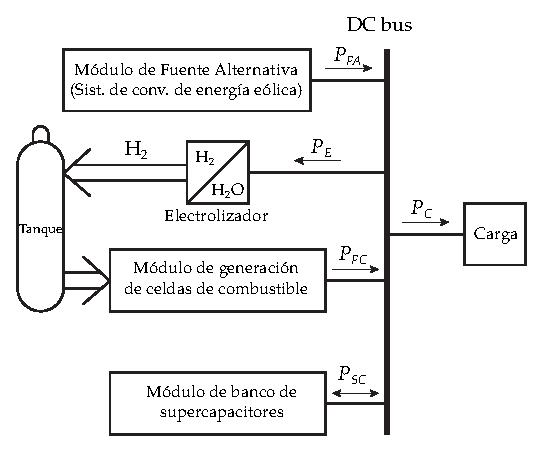
\includegraphics{gfx/diagrama_bloques_sistema_hibrido.eps}
 \caption{Diagrama en bloques de sistema híbrido}
 \label{fig:sist_hibrido}
\end{figure}

Para poder encarar la concepción del SGH se necesitarían todos los módulos que lo componen, esto representaría un gran costo. Por ello se ha
planteado una alternativa para el armado del sistema que consiste en la temporal sustitución de los módulos faltantes por plataformas de emulación.

\section{Emulador de pila de combustible}
El trabajo que se expone en el presente documento trata sobre el diseño y construcción de un emulador de pilas de combustible.
La necesidad del desarrollo de un emulador de pilas de combustible surge a partir de las diversas dificultades para obtener una pila
real, ya sea por su costo, su tamaño o el difícil acceso y almacenamiento del combustible.

La conexión de los módulos mostrados en la fig. \ref{fig:sist_hibrido} hacia el bus de tensión continua debe realizarse mediante una etapa de potencia 
que adapte los niveles eléctricos. En el proyecto del SGH, esta tarea ya ha sido abordada y constituyó el soporte para el desarrollo del emulador. 
La etapa de potencia consiste en un convertidor DC-DC conmutado elevador.

El flujo de trabajo del proyecto se llevó a cabo  de la siguiendo las tareas que se mencionan a continuación: en primer instancia se diseñaron los modelos
de simulación que luego fueron programados en el \emph{hardware} de control y se procedió a la realización de ciertos ajustes en la placa diseñada para el 
convertidor original cambiando la topología del mismo para permitirle funcionar según los modelos diseñados para finalmente realizar los ensayos finales.
\end{comment}

% Chapter 2

\chapter{Introducción a las antenas polarimétricas y sus problemas} % Chapter title
\label{ch:motivacion}
\lhead{\emph{Introducción a las antenas polarimétricas y sus problemas}}
%----------------------------------------------------------------------------------------

\section{Antenas polarimétricas}

Una antena polarimétrica es una antena que se la utiliza en radares y satélites. Generalmente trabajan en la
zona del espectro electromagnético de microondas. Las mismas pueden ser activas o pasivas, esto es, para el
primer caso, que el sistema emita su propia energía, para luego medir el eco de la misma. Para el segundo caso,
el radar no emite ninguna señal, simplemente recibe el eco de algún otro sistema emisor/receptor.

\begin{figure}[H]
 \centering
 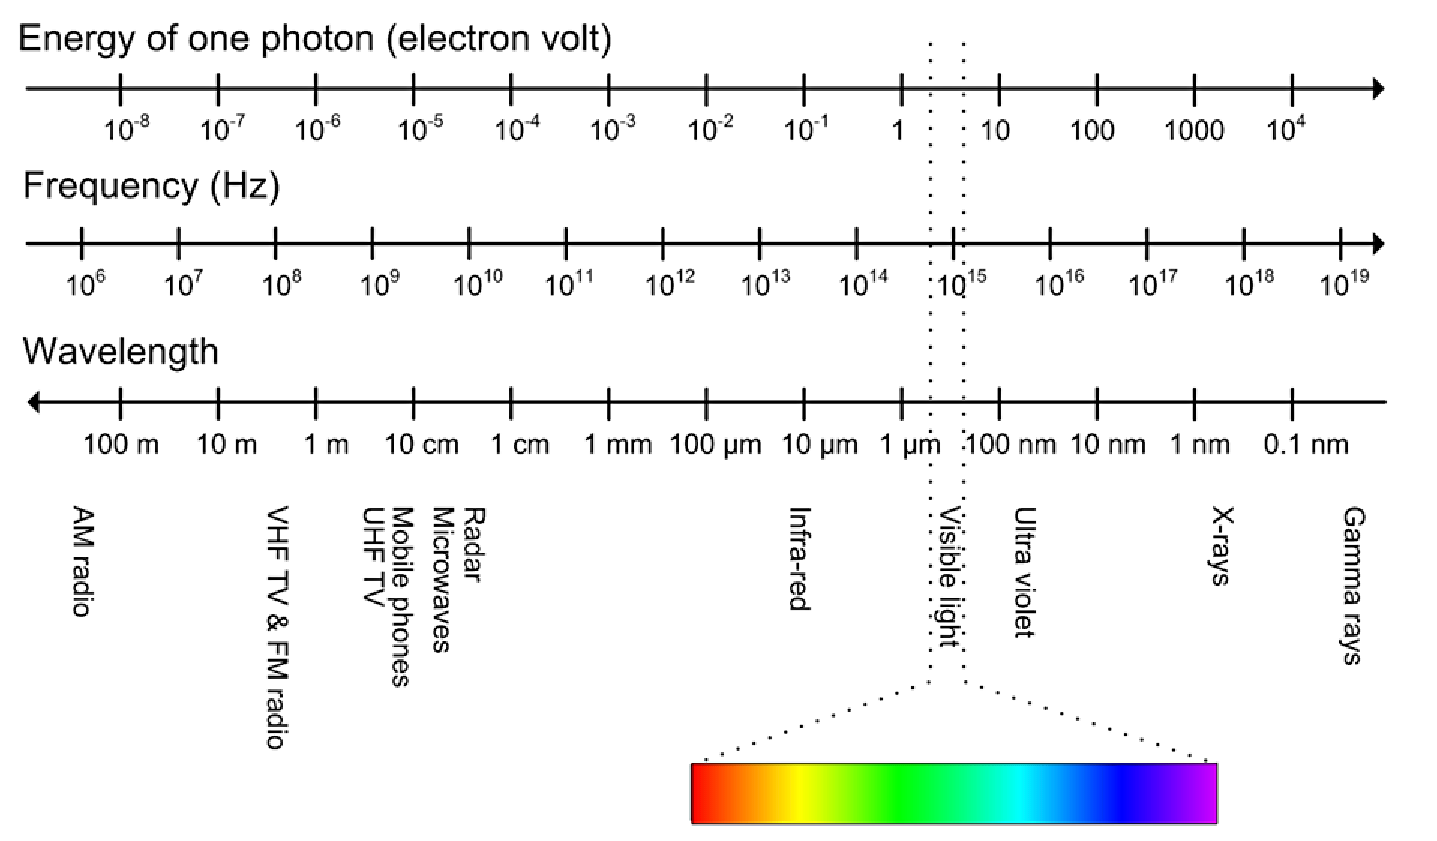
\includegraphics[width=10cm]{gfx/electromagneticSpectrum.png}
 \caption{Espectro Electromagnético}
 \label{fig:spectrum}
\end{figure}


Dado que la frecuencia de trabajo está comprende la región microondas del espectro electromagnético, el cual está entre los 
300 MHz y los 300 GHz (ver figura \ref{fig:spectrum}), y dado que en dicho rango la opacidad de la atmósfera es casi nula 
(ver figura \ref{fig:atmosphere}), estas antenas poseen la capacidad de trabajar independientemente de las condiciones 
atmosféricas, esto es, que la señal casi no es atenuada por la atmósfera, tampoco es interferida ni por las lluvias ni por 
las nubes. A su vez, se puede obtener información sobre la textura del terreno y sobre los sustratos inferiores de las 
coberturas boscosas. Dependiendo de que longitud de onda del rango de trabajo, se tiene de 3 cm a 30 cm de penetración.

\begin{figure}[H]
 \centering
 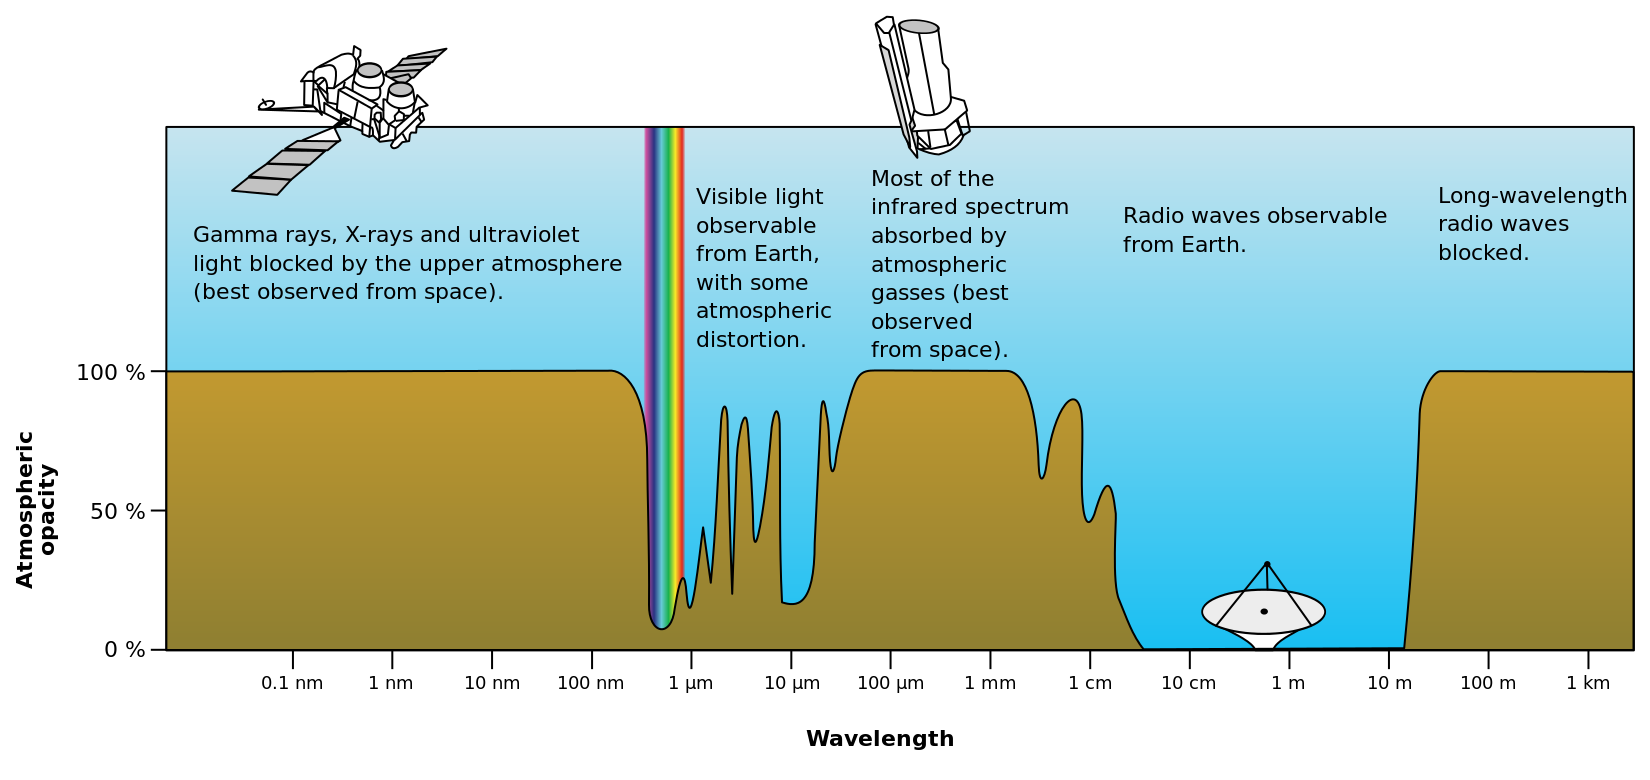
\includegraphics[width=10cm]{gfx/AtmosphericOpacity.png}
 \caption{Opacidad atmosférica vs longitud de onda}
 \label{fig:atmosphere}
\end{figure}

Por convención, el eje de referencia que es paralelo a la dirección del recorrido del satélite se lo llama azimuth. La
dirección del eje perpendicular, rango. El nadir es el punto más cercano de la tierra al satélite; en otras palabras, 
es el punto en la superficie terrestre que, si se trazara una recta perpendicular al mismo, también corta al satélite.

La antena nunca apunta diréctamente hacia abajo porque, de esta forma, se perdería mucha información en rango. Al apuntar 
en diagonal, y gracias a que el blanco no es puntual, el eco de la señal de la zona iluminada más cercana al nadir llega 
antes al satélite que la más alejada, logrando así, tomar muestras de distintos lugares espaciados en rango (ver figura 
\ref{fig:antena_ilumination}).

\begin{figure}[H]
 \centering
 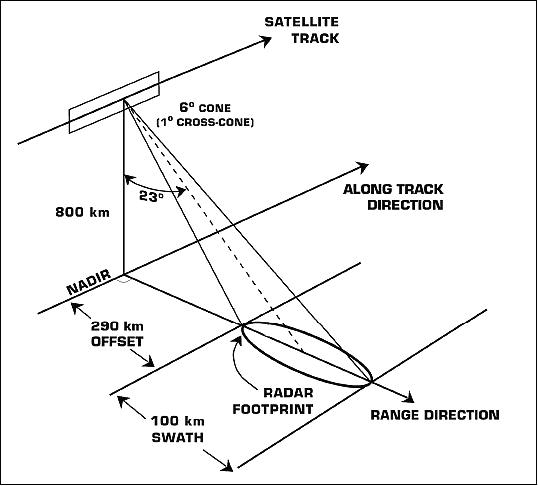
\includegraphics[width=7cm]{gfx/satellite.png}
 \caption{Footprint del satélite}
 \label{fig:antena_ilumination}
\end{figure}

El tamaño de la zona iluminada se llama footprint. Dicho tamaño depende tanto de las dimensiones de la antena como de la 
órbita del satélite o de la altura del avion en que está colocada dicha antena. Como se observa en la imagen 
\ref{fig:footprint}, mientras más larga es la antena, más angosto es el footprint, logrando así mejorar la resolución 
espacial.

\begin{figure}[H]
 \centering
 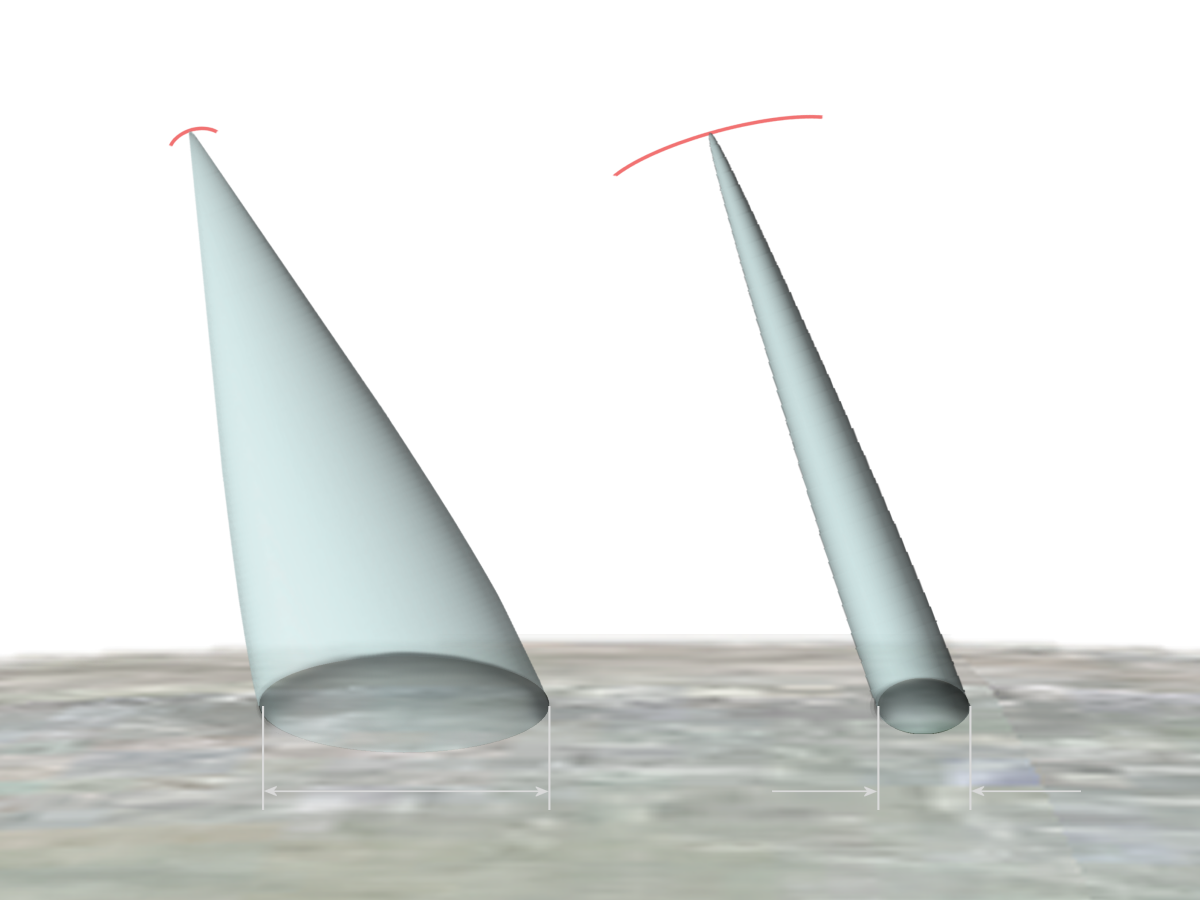
\includegraphics[width=7cm]{gfx/footprint.png}
 \caption{El footprint depende del largo de la antena}
 \label{fig:footprint}
\end{figure}

\subsection{Composición de una antena}

Un array de de una antena polarimétrica es una colección de N módulos radiantes espaciados. Todos los elementos poseen los
mismos patrones de radiación y están orientados en el mismo sentido y dirección en un ambiente tridimensional. No es 
necesario que los elementos estén espaciados regularmente ni que emitan los mismos valores de potencia y fase, pero se asume 
que todos están alimentados con la misma frecuencia de trabajo. En la figura \ref{fig:phasedArrayAntenna} se pueden observar
dos tipos de distribuciones comunmente utilizadas.

\begin{figure}[H]
	\centering
 	\subfloat[]{
		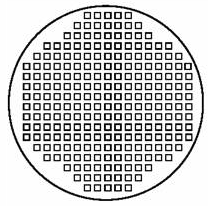
\includegraphics[width=4cm]{gfx/phasedArrayAntenna.png}}
	\subfloat[]{
		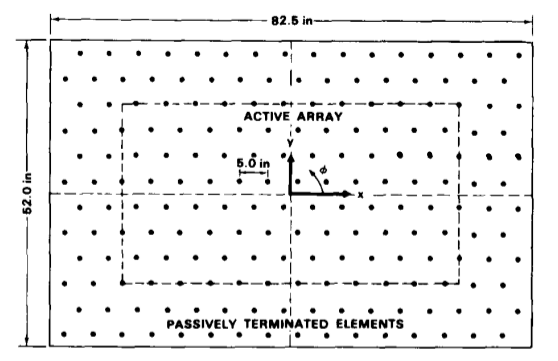
\includegraphics[width=6cm]{gfx/frontAntenna.png}}
	\caption{ (a) Antena de arreglo de fase circular. (b) Antena de arreglo de fase rectangular}
	\label{fig:phasedArrayAntenna}
\end{figure}

Este tipo de antenas están compuestas por tres bloques principales; los cuales son el generador, la red de distribución (o RFDN) y la 
antena con los módulos radiantes (ver figura \ref{fig:compositionAntenna}).

\begin{figure}[H]
 \centering
 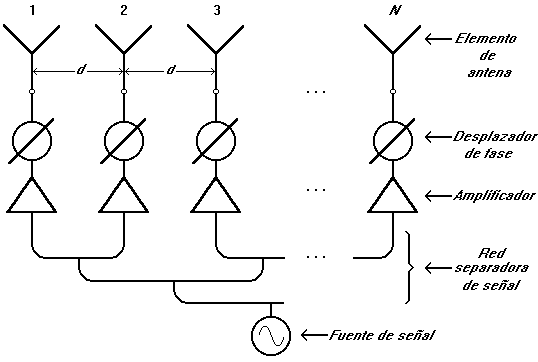
\includegraphics[width=10cm]{gfx/CompositionAntenna.png}
 \caption{Composición de un arreglo de antena}
 \label{fig:compositionAntenna}
\end{figure}

El generador de puede emitir distitnos tipos de modulaciones. Ej, cuadrada, chirp, senoidal, triangular, etc. Las ventajas y
desventajas de cada una se lista en el cuadro \ref{tab:modulations}

\begin{table}[H]
  \footnotesize
  \centering
  \begin{tabular}{|c|p{9cm}|}
	\hline
	\textbf{Modulación} & \textbf{Cacarcterísticas} \\
	Cuadrada & Esta modulación es utilizada para mediciones muy precisas a cortas distancias comparando las fases de los dos 
	semiciclos de la señal recibida. La desventaja es que los distintos ecos de los distintos blancos no pueden distinguirse.\\\hline
	Chirp & Es la modulación mayormente utilizada, se obtienen mediciones con las mayores distancias posibles.\\\hline
	Triangular & Con esta modulación se logra distinguir fácilmente la velocidad de la posición del blanco. \\\hline
	Escalonada & Es utilizada para mediciones de interferometría y para expandir el rango de medición sin ambig\"uedades.\\\hline
  \end{tabular}
  \caption{Cacacterísticas de cada modulación de la señal emitida}
  \label{tab:modulations}
\end{table}

La red de distribución, llamada RFDN, es la encargada de transmitir la señal a todos los módulos radiantes de la antena. 
Dicha red posee una estructura de árbol, de forma tal, que la longitud de todos los caminos entre las hojas del mismo a 
la raíz son iguale (Los nodos son los PSC y las holas los RMs). Es necesraio que todos los caminos sean iguales para que la 
señal transmitida posea la misma fase y atenuación. Los componentes utilizados para distribuir la señal son los siguientes:

\begin{itemize}
	\item Power Splitter Combiner: este componente es el encargado de dividir la señal transmitida en tantos puertos de salida 
		tenga y la de sumar/combinar las potencias recibidas.
	\item Cable: este componente es el utilizado para unir el resto de los componentes.
	\item Módulo de Transmisión y Recepción: Este componente es el encargado de atenuar y amplificar la señal para que, tanto
		la potencia transmitida como la entrante a la red esté controlada y conocida. Hay uno por cada módulo radiante para 
		poder calibrar la antena, esto es, que la potencia de salida/entrada sea la misma en cada módulo radiante.
	\item Defasador: Este componente simplemente defasa la señal transmitida, hay uno por cada módulo radiante, se lo utiliza
		para poder calibrar la antena tanto en transmisión como en recepción, logrando así, que cada camino de transmisión/
		recepción de las hojas a la raíz defase lo mismo. A su vez, se lo utiliza para poder direccionar el beam de la señal
		emitida.
	\item Módulo Radiante: Este componente es el emisor de la señal a transmitir y/o el receptor. En este tipo de antenas un 
		RM puede cumplir una o ambas funcionalidades.
	\item Circulador: Este componente generalmente es uno de tres puertos, se lo utiliza para separar los caminos de la 
		señal transmitida (Tx) de la recibida (Rx). Generalmente es utilizado si el mismo módulo radiante se lo utiliza para
		transmisión como recepción.
\end{itemize}

Se pueden armar los módulos de tal forma que puedan transmitir en dos polarizaciones distintas, H y V (Ver figura 
\ref{fig:polarizations}), para esto, se debe duplicar la RFDN. Haciendo uso de ambas polarizaciones se puede caracterizar 
los blancos observados, dado que, cada cuerpo responde de forma distinta a cada tipo de polarización.

\begin{figure}[H]
 \centering
 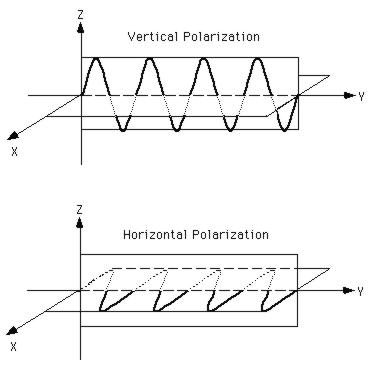
\includegraphics[width=7cm]{gfx/HAndVPolarizations.png}
 \caption{Polarizaciones verticales y horizontales}
 \label{fig:polarizations}
\end{figure}



\subsection{Patrón de antena}

Un array de antena puede armarse recursivamente, esto es, que un elemento sea, en si mismo, un array. Un patrón de antena es 
un patrón de radiación polar que resulta de reemplazar cada elemento por un radiador isotrópico. Si se asume que el patrón de
radiación de cada elemento es idéntico al del resto, tomando una cierta incertidumbre, el patrón de radiación total resulta de
la multiplicación de todos los patrones de todos los elementos. Este resultado no depende de si se consideran los patrones de
potencia o de amplitud/fase.

A continuación se mostrarán gráficos representando la potencia del campo radiado, asumiendo campo lejano. La potencia decae 
con la relación de $1/r$, donde $r$ es la distancia del punto de medición al elemento radado. Se debe tomar en cuenta también
la fase con que emite el elemento y el retardo de fase que se debe al tiempo en que tarda en llegar la señal a los distintos 
lugares del espacio. El retardo es expresado como $2\pi r/\lambda$, siendo $\lambda$ la longitud de onda de la señal emitida 
por el elemento radiado. Los gráficos \ref{fig:twoArrayPat} y \ref{fig:fourArrayPat} muestran las curvas de nivel de patrones 
de radiación de pontencia polar. La separación de los módulos radiantes está en el eje x, eje horizontal y todos los elementos
están emitiendo en fase.


\begin{figure}[H]
	\centering
	\subfloat[]{
		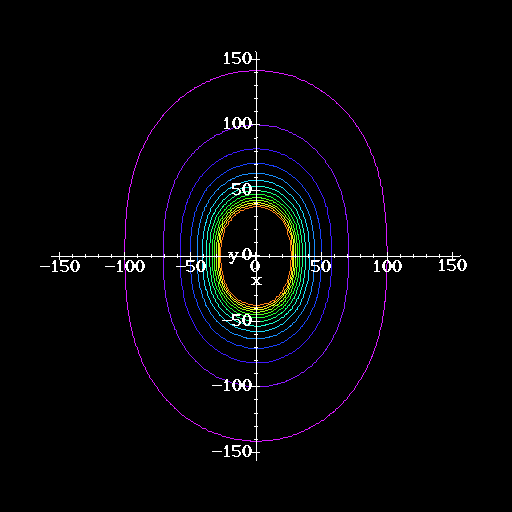
\includegraphics[width=5cm]{gfx/TwoIsoQuartDist.png}}
	\subfloat[]{
		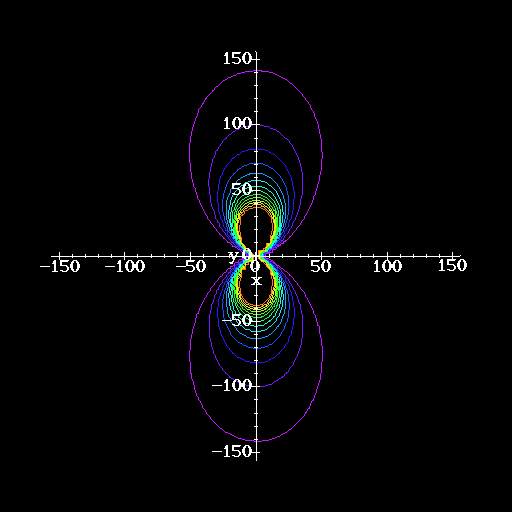
\includegraphics[width=5cm]{gfx/TwoIsoHalfDist.png}}
	\caption{Patrones de radiación de potencia. a) Dos elementos radiantes separados $1/4$ de longitud de onda, b)
	Dos elementos radiantes separados $1/2$ de longitud de onda}
	\label{fig:twoArrayPat}
\end{figure}

\begin{figure}[H]
	\centering
	\subfloat[]{	
		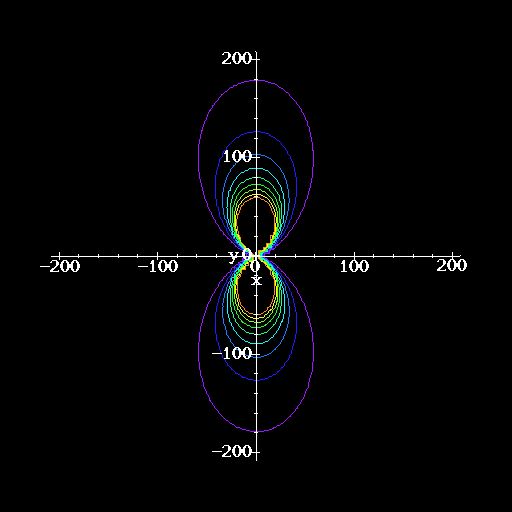
\includegraphics[width=5cm]{gfx/FourIsoQuartDist.png}}
	\subfloat[]{	
		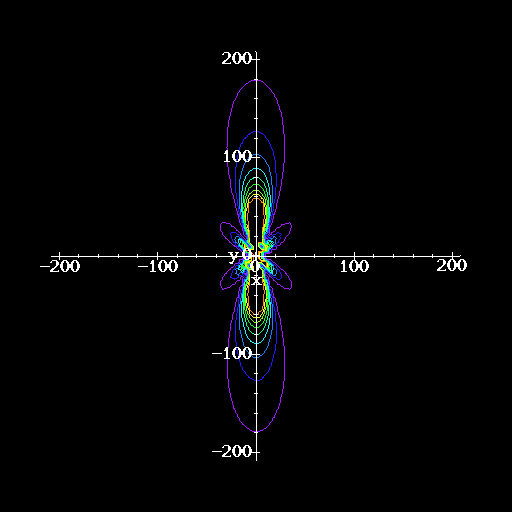
\includegraphics[width=5cm]{gfx/FourIsoHalfDist.png}}
	\caption{Patrones de radiación de potencia. a) Cuatro elementos radiantes separados $1/4$ de longitud de onda, b)
	Cuatro elementos radiantes separados $1/2$ de longitud de onda}
	\label{fig:fourArrayPat}
\end{figure}

Se puede observar que aumentando la cantidad de módulos radiantes, se logra que el beam principal (lóbulo principal de 
potencia), sea más angosto, por lo tanto se obtenga una mayor resolución del cuerpo observado. Observando la siguiente 
figura (\ref{fig:directArrayPat}), se puede deducir que la fase de los elementos radiados modifica la dirección del 
patrón de antena.

\begin{figure}[H]
	\centering
	\subfloat[]{	
		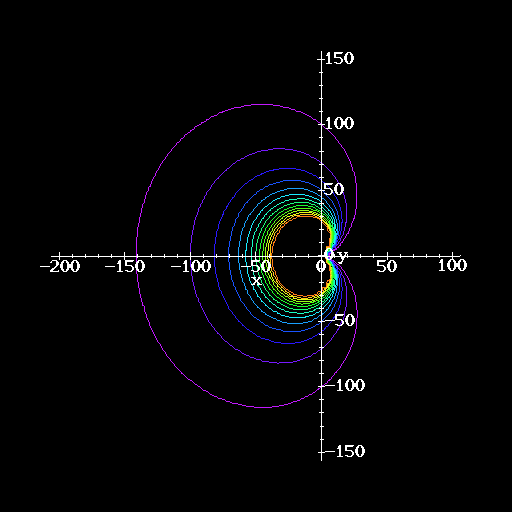
\includegraphics[width=5cm]{gfx/TwoQuarterPhase.png}}
	\subfloat[]{	
		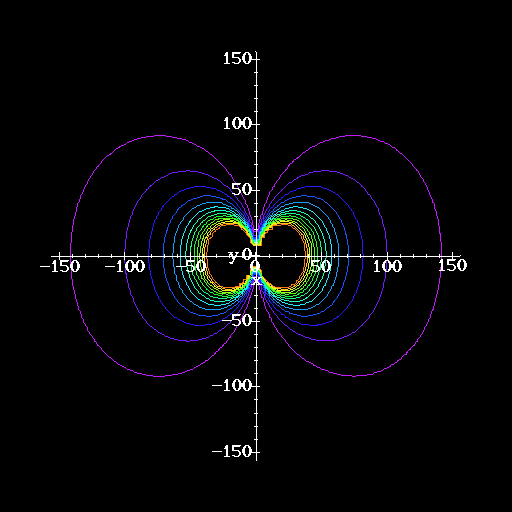
\includegraphics[width=5cm]{gfx/TwoAntiPhase.png}}
	\caption{Patrones de radiación de potencia. a) Dos elementos radiantes separados $1/4$ de longitud de onda y con 
		defasaje de $\pi$, b) Dos elementos radiantes separados $1/2$ de longitud de onda y en contrafase}
	\label{fig:directArrayPat}
\end{figure}

\todo[inline]{Aca faltó algo importantísimo, que es agregar lo importante del patrón de antena, un paper dice lo siguiente:}
\todo{agregar definiciones de directividad}
Directividad, el ancho del lóbulo principal, y el nivel de los lóbulos secundarios son los tres parámetros más importantes 
de una antena de arreglo de fase \cite{Hsiao1985}.

Lamentablemente los errores del arreglo limitan los niveles que se pueden obtener de los lóbulos secundarios \cite{Hsiao1985}.

Como es bien sabido, si se achican los lóbulos secundarios, tanto la directividad como el ancho del lóbulo principal son
afectados. Para mantener ambas características invariantes, es necesario increentar el tamaño de la antena de arreglo de 
fase \cite{Hsiao1985}.

\section{Parámetros S}

La sigla S deriva de la palabra scattering. Para altas frecuencias, es conveniente describir una
determinada red en términos de ondas en vez de tensiones o corrientes. Esto permite una definición más 
sencilla de planos de referencia. Por razones prácticas, la descripción en términos de ondas entrantes
y salientes ha sido introducida. Ahora, una red de 4 polos se transforma en 2 puertos y $2n$ polos se 
transforman en $n$ puertos. En el caso de un número impar de polos (ej. 3 polos), un punto de referencia
puede ser elegido, atribuyendo un polo igualmente a dos puertos. Por lo tanto 3 polos se convierten en 
3 + 1 polo correspidiendo a 2 puertos. Como una regla general, para cantidades impares de polos, siempre
se agrega un polo extra.

\begin{figure}[H]
 \centering
 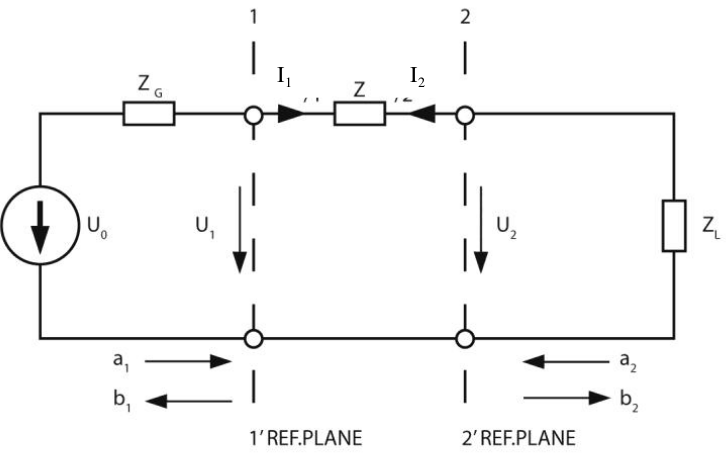
\includegraphics[width=10cm]{gfx/sParameters1.png}
 \caption{Ejemplo de una red de 2 puertos: circuito serie}
 \label{fig:esquema_serie}
\end{figure}

Tomando como ejemplo una red de 2 puertos compuesta por una sola impedancia $Z$ conectada en serie (\ref{fig:esquema_serie}).
Las impedancias de la fuente y de la carga son $Z_G$ y $Z_L$ respectivamente. Si $Z=0$ y $Z_L = Z_G$ (para el caso de $Z_G$ real) 
la carga está adaptada. En este caso se obtiene una máxima transferencia de potencia y $U_1 = U_2 = U_0/2$. Notar que todas las
tensiones y corrientes son valores pico. Se supone que las líneas que unen los componentes poseen longitud eléctrica igual a 0. 
Las conecciones con una longitud eléctrica finita están dibujadas como una doble líea. A continuación se relacionará $U_0$, $U_1$ 
y $U_2$ a $a$ y $b$.


\subsection{Definición de \enquote*{ondas de potencia}}

Las ondas incidentes al puerto son $\textbf{a}=(a_1, a_2, a_3, ..., a_n)$, las ondas salientes, o reflejadas, del puerto son  
$\textbf{b}=(b_1, b_2, b_3, ..., b_n)$. Por definición, las corrientes incidentes son positivas y las salientes negativas. La
onda $a_1$, incidente al puerto 1, es derivada de la tensión entrante a la carga balanceada. 

Para hacer qe esta definición sea consistente con la ley de la conservación de la energía. La tensión es normalizada a $\sqrt{Z_0}$. 
$Z_0$ es, en general una impedancia de referencia arbitraria, que usualmente se la utiliza como la impedancia característica de la 
línea (ej, $Z_0 = 50 \Omega$). Y, cuando todas las impedancias son iguales ($Z_G = Z_L = Z_0$), se dice que la línea está adaptada
y no hay onda reflejada. Las definiciones de $a1$ y $b1$ son:

\begin{equation}
\begin{aligned}
	a1 &= \dfrac{U_0}{2\sqrt{Z_0}}= \dfrac{\textrm{onda de tensión incidente (puerto 1)}}{\sqrt{Z_0}}=\dfrac{U_1^{inc}}{\sqrt{Z_0}} \\
	b1 &= \dfrac{U_1^{refl}}{2\sqrt{Z_0}}= \dfrac{\textrm{onda de tensión reflejada (puerto 1)}}{\sqrt{Z_0}}
\end{aligned}
\end{equation}

Notar que \textbf{a} y \textbf{b} tienen las unidades de $\sqrt{\textrm{potencia}}$.

La potencia incidente al puerto 1, $P_{inc}$, es simplemente la potencia entregada por la fuente, mientras que la potencia saliente 
del puerto 1, $P_{refl}$, viene de la onda de tensión reflejada.

\begin{equation}
\begin{aligned}
	P_1^{inc} &= \dfrac{1}{2}|a_1|^2= \dfrac{|U_1^{inc}|^2}{2Z_0}=\dfrac{|I_1^{inc}|^2}{2}Z_0 \\
	P_1^{refl} &= \dfrac{1}{2}|b_1|^2= \dfrac{|U_1^{refl}|^2}{2Z_0}=\dfrac{|I_1^{refl}|^2}{2}Z_0 \\
\end{aligned}
\end{equation}

En el caso de una desadaptación de la impedancia de carga $Z_L$, parte de la potencia será reflejada a través del puerto 2 (
potencia incidente al puerto 2).

$$
P_2^{inc}=\dfrac{1}{2}|a_2|^2
$$

Se ha definido $a_1 = U_0/2\sqrt{Z_0} = U^{inc}/\sqrt{Z_0}$ con la onda de tensión incidente $U^{inc}$. Como analogía 
se la puede definir como $a_1 = I^{inc}\sqrt{Z_0}$ con la onda incidente de corriente $I^{inc}$. Utilizando ambas, se obtiene la 
definición general de las ondas incidentes $a_i$ y reflejadas $b_i$ de un puerto.

\begin{equation}
\begin{aligned}
	a_i &= \dfrac{U_i + I_iZ_0}{2\sqrt{Z_0}} \\
	b_i &= \dfrac{U_i - I_iZ_0}{2\sqrt{Z_0}}
\end{aligned}
\label{eq:waves}
\end{equation}

Solucionando este sistema de ecuaciones, $U_i$ y $I_i$ pueden ser obtenidas de $a_i$ y $b_i$ como

\begin{equation}
\begin{aligned}
	U_i &= \sqrt{Z_0}(a_i + b_i) = U_i^{inc} + U_i^{refl}\\
	I_i &= \dfrac{1}{\sqrt{Z_0}}(a_i - b_i) = \dfrac{U_i^{refl}}{Z_0}
\end{aligned}
\end{equation}


\subsection{La matríz de parámetros S}

La relación entre $a_i$ y $b_i$ (siendo $i=1..n$) puede ser escrito como un sistema de n ecuaciones lineales (siendo la variable 
independiente $a_i$ y $b_i$ como la dependiente)

\begin{equation}
\begin{aligned}
	b_1 = S_{11}a_1 + S_{12}a_2 \\
	b_2 = S_{21}a_1 + S_{22}a_2
\end{aligned}
\label{eq:s_matrix}
\end{equation}
	
Escrito de forma matricial: \textbf{b} = \textbf{Sa}

El significado físico de los parámetros S son los siguientes:
\begin{itemize}
	\item $S_{11}$: es el coeficiente de reflexión con la salida de la red terminada en una carga adaptada ($a_2 = 0$).
	\item $S_{21}$: es la transmisión en directa (del puerto 1 al 2)
	\item $S_{12}$: es la transmisión en inversa (del puerto 2 al 1)
	\item $S_{22}$: es el coeficiente de reflexión de la salida. 
\end{itemize}

Al medir todos los parámetros S de una red de n puertos, todos los puertos deben estar terminados con una carga adaptada.
Utilizando las equaciones \ref{eq:waves} y \ref{eq:s_matrix} se obtiene el coeficiente de reflexión de una impedancia $Z_L$
conectada a un generador de impedancia de salida $Z_0$ (Figura \ref{fig:esquema_serie}, caso $Z_G = Z_0$ y $Z = 0$):

\begin{equation}
S_{11} = \dfrac{b_1}{a_1}\bigg|_{a_2=0} = \dfrac{U_1 - I_1Z_0}{U_1 + I_1Z_0} = \dfrac{Z_L - Z_0}{Z_L + Z_0} = \Gamma 
\end{equation}

\subsection{La matriz de transferencia}

Resulta muy conveiente la utilización de la matriz de parámetros S para describir una red de n polos en términos de ondas y 
para mediciones. Pero, no es muy conveniente su utilización para caracterizar la respuesta de una cascada de redes de 2 
puertos. En este caso, una manera de encarar dicha problemática, es la utilización de la matriz de parámetros T (matriz 
de transferencia), la cual relaciona las ondas de entrada y salida de cada cuadripolo.

\begin{equation}
\begin{pmatrix} a_1\\b_1 \end{pmatrix} = \begin{pmatrix} T_{11} & T_{12}\\T_{21} & T_{22} \end{pmatrix} 
\begin{pmatrix} a_2\\b_2 \end{pmatrix}
\end{equation}

Cabe destacar que, para los casos en que no hay transmisión entre el puerto 1 y 2, si bien la matriz de parámetros S está definida, 
la matriz de parámetros T no. La matriz resultante de parámetros T de una cascada de redes de 2 puertos resulta como sigue:

\begin{equation}
\mathbf{T_M=T_1T_2...T_m}
\end{equation}

\subsection{Conversión entre parámetros T y S}

Como la matriz de transferencia (T) simplemente relaciona las ondas de entrada y salidas de una forma diferente a la matriz de 
scattering, partiendo de una matriz se puede llegar a la otra y viceversa.

\begin{equation}
	\begin{aligned}
		T_{11} &= S_{12} - \dfrac{S_{22}S_{11}}{S_{21}},\quad T_{12} = \dfrac{S_{11}}{S_{21}} \\
		T_{21} &= - \dfrac{S_{22}}{S_{21}},\qquad\qquad T_{22} = \dfrac{1}{S_{21}}
	\end{aligned}
\end{equation}

Para obtener los parámetros S partiendo desde los parámetros T, se utiliza la siguiente relación matemática

\begin{equation}
	\begin{aligned}
		S_{11} &= \dfrac{T_{12}}{T_{22}},\qquad S_{12} = T_{11} - \dfrac{T_{12}T_{21}}{T_{22}} \\
		S_{21} &= \dfrac{1}{T_{22}},\qquad S_{22} = - \dfrac{T_{21}}{T_{22}}
	\end{aligned}
\end{equation}


\subsection{Propiedades de la matriz de parámetros S}

Una red generalizada de n puertos posee $n^2$ coeficientes de scattering. Mientras que los $S_{ij}$ podrían ser todos independientes,
en general, debido a simetrías u otros factores, la cantidad de coeficientes independientes es mucho menor.
\begin{itemize}
	\item Una red de n puertos es recíproca cuando $S_{ij} = S_{ji}$ para todo $i, j$. La mayoría de los componentes pasivos son 
		recíprocos (resistencias, capacitores, transformadores, etc., exceptuando para estructuras involucrando ferrites magnéticos,
		plasmas, etc.), componentes activos como amplificadores generalmente son no recíprocos.
	\item Una red de 2 puertos es simétrica cuando es recíproca ($S_{21} = S_{12}$) y cuando los coeficientes de reflexión son iguales
		($S_{11} = S_{22}$).
	\item Una red de N puertos es pasiva y sin pérdidas si su matriz de parámetros S es unitaria ($\mathbf{S^{\dagger}S = 1}$ donde 
		$\mathbf{x^{\dagger} = (x^*)^T}$ es la conjugada y transpuesta de $x$). Para una red de 2 puertos esto significa

\begin{equation}
S^{\dagger}S = \begin{pmatrix} S_{11}^* & S_{21}^*\\S_{12}^* & S_{22}^* \end{pmatrix}
			\begin{pmatrix} S_{11} & S_{12}\\S_{21} & S_{22} \end{pmatrix} = \begin{pmatrix} 1 & 0\\0 & 1 \end{pmatrix}
\end{equation}

Esto conlleva a 3 condiciones 

\begin{equation}
\begin{aligned}
	|S_{11}|^2 + |S_{21}|^2 = 1 \\
	|S_{12}|^2 + |S_{22}|^2 = 1 \\
	S_{11}^*S_{12} + S_{21}^*S_{22} = 0
\end{aligned}
\label{eq:sCondition}
\end{equation}

Separando la última ecuación en módulo y fase, se obtiene

\begin{equation}
\begin{aligned}
	|S_{11}||S_{12}| &= |S_{21}||S_{22}| \\
	-argS_{11} + argS_{12} &= -argS_{21} + argS_{22} + \pi
\end{aligned}
\label{eq:con}
\end{equation}

Donde $arg(x)$ es el argumento (angulo) de la variable compleja $x$. Combinando la ecuación \ref{eq:sCondition} con la primera 
de la ecuación \ref{eq:con} se obtiene

\begin{equation}
\begin{aligned}
	|S_{11}| = |S_{12}|, |S_{21}| = |S_{22}| \\
	|S_{11}| = \sqrt{1 - |S_{12}|^2}
\end{aligned}
\end{equation}

Por lo tanto, cualquier red de 2 puertos sin pérdidas puede ser caracterizada con un módulo y tres ángulos.
\end{itemize}

En general los parámetros S son valores complejos y dependientes de la frecuencia. 

\section{Parámetros S de cada componente}

Los componentes que son ideales, se los trata como si estuviesen perfectamente adaptados, logrando así que los coeficientes
de reflexión sean nulos, esto es $S_{11} = S_{22} = 0$

\subsection{RM}
	
El módulo radiante es un módulo de un único puerto y es pasivo, por lo tanto el parámetro S que lo define es $S_{11}$ y su 
valor varía entre -1 y 1.

\begin{itemize}
	\item Cortocircuito ideal: $S_{11} = -1$
	\item Conexión ideal: $S_{11} = 0$
	\item Circuito abierto ideal: $S_{11} = 1$
\end{itemize}

Los casos de cortocircuito y circuito abierto son casos de falla del módulo radiante. Cualquier otro valor intermedio implica
una desadaptación de impedancias.

\subsection{Cable ideal}
Un cable se comporta como una línea de transmisión, y su matriz es la siguiente

$$
\mathbf{S} = \begin{pmatrix} 0 & e^{-\gamma l}\\e^{-\gamma l} & 0\end{pmatrix}
$$

Donde $\gamma = \alpha + j\beta$ es una constante de propagación compleja. $\alpha$ es la atenuación de la línea en [neper/m] 
y $\beta = 2\pi/\delta$ con la longitud de onda $\delta$. Para una línea sin pérdidas se obtiene $|S_{21}| = 1$

\subsection{Phase shifter ideal}

$$
\mathbf{S} = \begin{pmatrix} 0 & e^{-j\phi_{12}}\\e^{-j\phi_{21}} & 0\end{pmatrix}
$$

Un defasador recíproco posee $\phi_{12} = \phi_{21}$.

\subsection{Atenuador ideal}

$$
\mathbf{S} = \begin{pmatrix} 0 & e^{-\beta}\\e^{-\alpha} & 0\end{pmatrix}
$$

Si el atenuador es recíproco, $\alpha = \beta$. El factor de atenuación, $\alpha$, está en neper. La atenuación en decibeles
viene dado por $A = '20\log_{10}(S_{21})$, $1N = 8.686dB$.


\subsection{Amplificador ideal}

$$
\mathbf{S} = \begin{pmatrix} 0 & 0\\G & 0\end{pmatrix}
$$

Con $G > 1$.


\subsection{Circulador ideal}

El circulador ideal es sin pérdidas y adaptado en todos sus puertos. La señal entrante por un puerto es exclusivamente 
transmitida al puerto siguiente en el sentido de la flecha.

\begin{figure}[H]
 \centering
 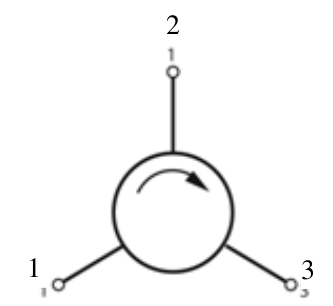
\includegraphics[width=4cm]{gfx/circulator.png}
 \caption{circulador de 3 puertos}
 \label{fig:circulator}
\end{figure}

La matriz de parámetros S es como sigue.

$$
\mathbf{S} = \begin{pmatrix} 0 & 0 & 1\\1 & 0 & 0\\0 & 1 & 0\end{pmatrix}
$$


\subsection{PSC}

El tipo de PSC modelado consiste en una red recíproca y adaptada en todos sus puertos, pero con pérdidas. Puede ser un 
componente de 3 o más puertos. A continuación se muestra la matriz de parámetros S genérica para una red de n puertos 
(matriz de nxn).

$$
\mathbf{S} = \begin{pmatrix} 0 & \dfrac{1}{n-1} & ... & \dfrac{1}{n-1}\\
							 \dfrac{1}{n-1} & 0 & ... & \dfrac{1}{n-1}\\
							 ... & ... & ... & ... \\
							 \dfrac{1}{n-1} & \dfrac{1}{n-1} & ... & 0 \end{pmatrix}
$$

\begin{comment}
El descubrimiento de la celda de combustible derivó de un experimento de electrólisis, proceso en el que se utiliza corriente
eléctrica para producir la separación de los compuestos en sus elementos. El hecho que llevó a descubrir el principio de la celda
de combustible fue la reversibilidad (en términos cualitativos) del proceso, es decir que pudo obtenerse energía eléctrica de
la reacción que devolviera los elementos al compuesto original.

La reacción química llevada a cabo es la misma que si el proceso fuese realizado mediante la combustión de los reactivos. 
Pero se distingue de éste último proceso en que parte de la energía liberada es eléctrica.
Por otra parte, la reversibilidad del proceso le confiere características particulares. Una de ellas
es que su eficiencia no está limitada por el ciclo de Carnot, como es el caso de los procesos termodinámicos.

\section{Principios de funcionamiento}

El dispositivo esta constituido básicamente por dos partes fundamentales: el electrolito y los electrodos. El electrolito es
el material que facilita el movimiento de iones y los electrodos ofrecen una superficie para la posibilitar la reacción química.
La reacción producida por las celdas más elementales y las de interés para este trabajo es la siguiente:

$$
2H_{2}+O_{2} \rightarrow 2H_{2}O
$$

Ésta última expresión sirve para ilustrar la simplicidad de los procesos químicos que se llevan a cabo en estos dispositivos.
El esquema de una celda de combustible elemental de electrolito ácido se muestra en la fig. \ref{fig:esquema_celda} con las
reacciones que entran en juego y el modo en que se da el flujo de los reactivos y productos entregando corriente eléctrica
a la carga conectada.

\begin{figure}[H]
 \centering
 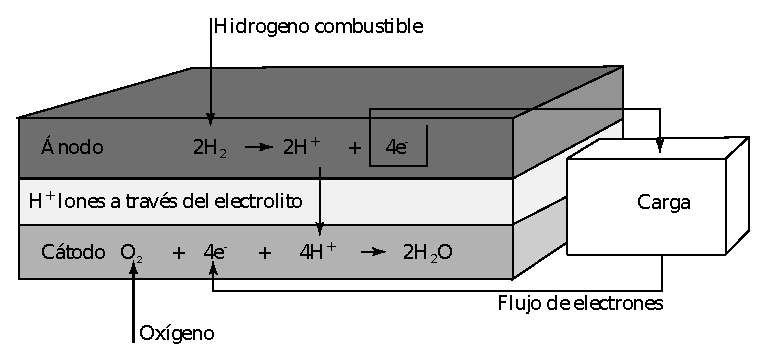
\includegraphics[width=10cm]{gfx/esquema_celda.eps}
 \caption{Esquema constructivo de una celda de combustible de electrolito ácido}
 \label{fig:esquema_celda}
\end{figure}

En el esquema de la fig. \ref{fig:esquema_celda} se analiza con mayor detalle las reacciones puestas en juego que se transcriben
en las ecuaciones \ref{eq:reacciones}.

\begin{subequations}
 \begin{equation}
  2H_2 \rightarrow 4H^{+}+4e^{-}
  \label{eq:reaccion_hidrogeno}
 \end{equation}
 \begin{equation}
  O_2+4H^{+}+e^{-} \rightarrow H_{2}O
 \end{equation}
 \begin{equation}
  2H_2+O_2 \rightarrow H_{2}O+ \Delta \overline{g}_f
  \label{eq:reaccion_basica}
 \end{equation}
 \label{eq:reacciones}
\end{subequations}

En ( \ref{eq:reaccion_basica}) se ha adicionado el término $\Delta \overline{g}_f$ que representa la energía de formación. 
Éste término es negativo para la reacción en cuestión, es decir que se libera energía de la reacción estudiada. Ésta energía
se manifiesta de diferentes maneras.

A pesar de tratarse de una reacción espontánea no se lleva a cabo a menos que se suministre la energía de activación necesaria
para que se produzca, y esto limita su ritmo. Para que aumente la probabilidad de que la reacción tenga lugar pueden
tomarse medidas como:
\begin{itemize}
 \item El aumento del área efectiva de los electrodos
 \item El aumento de la temperatura
 \item El uso de catalizadores
\end{itemize}

Si bien las celdas de combustible efectivamente proveen energía eléctrica, lo hacen en pequeñas cantidades. La tensión entregada entre
los terminales de sus electrodos es del orden de $1V$ y es por ello que normalmente las celdas de combustible se suelen configurar en
arreglos de \emph{pilas de celdas de combustible}, cuyas celdas son interconectadas en serie para que de los electrodos terminales 
se obtenga la suma de la tensión que entrega cada una de ellas.

Considerando la reducida tensión que entregan las celdas se disponen en pilas usando conectores especiales que limitan la caída de tensión
entre los contactos de cada electrodo. Una de las disposiciones típicas de las pilas de celdas es la que se muestra en la fig. \ref{fig:apilado}.

\begin{figure}[H]
 \centering
 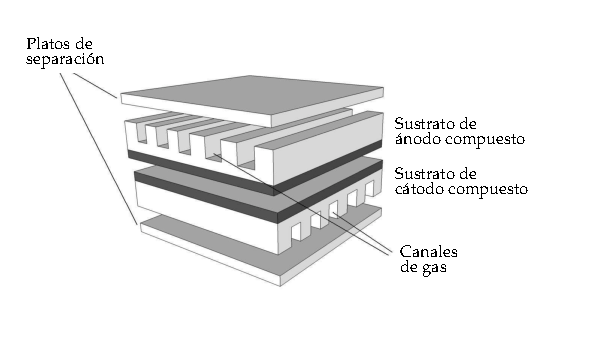
\includegraphics{gfx/apilado_bipolar_planar.eps}
 \caption{Disposición en apilado bipolar planar}
 \label{fig:apilado}
\end{figure}

\section{Tipos de celdas de combustible}
Para hacer frente a las dificultades presentadas en el desarrollo de las celdas de combustible, se probaron varias tecnologías dando
lugar a varios tipos de celdas de combustible. Éstas se diferencian especialmente por el electrolito utilizado y por ende el tipo
de ion que se mueve a través de él. En el cuadro \ref{tab:tipos_de_celdas} se listan las celdas típicas que pueden encontrarse.

\begin{table}[H]
 \centering
 \rowcolors{1}{}{gray!20}
 \begin{tabular}{|p{4cm}|p{1cm}|p{3cm}|p{5cm}|} \hline
 \rowcolor{LightBlue2} Tipo de celda de combustible	& Ion móvil	&Temperatura de operación	&Aplicaciones \\ \hline
 Alcalina (AFC)						& $ OH^{-} $	&$50-200$\textcelsius		&Usada en vehículos espaciales \\
 Membrana de intercambio de protones (PEMFC)		& $ H^{+} $	&$30-100$\textcelsius		&Vehículos, aplicaciones móviles y sistemas de baja potencia \\
 Metanol directo (DMFC)					& $ H^{+} $	&$20-90$\textcelsius		&Apropiado para sistemas de electrónica portátil de bajo consumo \\
 Ácido fosfórico (PAFC)					& $ H^{+} $	&\texttildelow$220$\textcelsius	&Sistemas de cogeneración de 200kW \\
 Carbonato fundido (MCFC)				& $ CO_3^{2-}$	&\texttildelow$650 $\textcelsius&Sistemas de cogeneración de hasta MW de capacidad \\
 Óxido sólido (SOFC)					& $ O^{2-} $	&$500-1000$\textcelsius		&Sistemas de cogeneración de 2kW a varios MW \\ \hline
 \end{tabular}
 \caption{Clasificación de los tipos de celdas de combustible}
 \label{tab:tipos_de_celdas}
\end{table}

Existen otros tipos de celdas además de los mencionados en el cuadro \ref{tab:tipos_de_celdas} aunque en este trabajo solo se ocupó de las
celdas de Membrana de intercambio Protónico (PEM). Las pilas de celdas PEM son muy sencillas de operar y funcionan a bajas temperaturas.
Además ofrecen un amplio rango de potencias según el tamaño. Se componen por un electrolito solido y los electrodos usan pequeñas cantidades
de platino como catalizador. Sin embargo es necesario que el hidrógeno suministrado sea de muy alta pureza, lo cual trae ciertas complicaciones.

\section{Sistemas de celdas de combustible}
Las partes fundamentales de la celda han sido enumeradas y explicadas tanto como su funcionamiento. Sin embargo las celdas requieren de varios
subsistemas auxiliares que se encarguen de regular todas las magnitudes de entrada a la pila. El diseño y correcto funcionamiento conjunto de estos
módulos representa un complejo problema de ingeniería. Un esquema sencillo de un sistema de celdas se muestra en la fig. \ref{fig:sistema_pila}.

\begin{figure}[H]
 \centering
 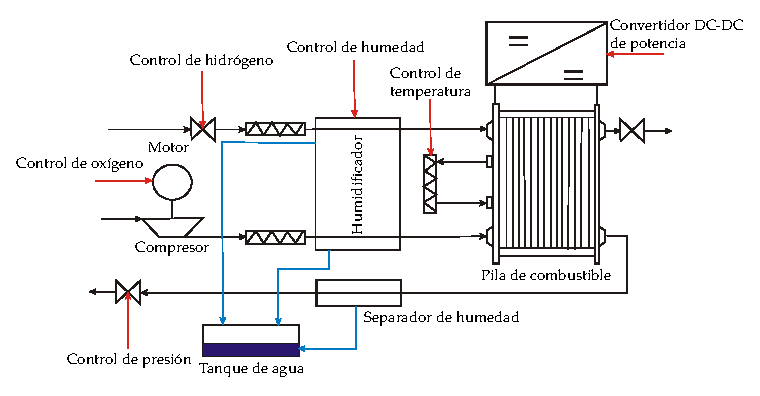
\includegraphics[width=11cm]{gfx/sistema_de_pila_de_combustible.eps}
 \caption{Sistema de celdas de combustible tipo PEM}
 \label{fig:sistema_pila}
\end{figure}

Aunque esos componentes auxiliares pueden variar, se explican los que se presentan en la mayoría de los sistemas:

\begin{itemize}
 \item \textbf{Suministro de combustible}: Se encarga de proporcionar el combustible con la pureza y la presión apropiadas hacia
 el colector. Para el caso de las PEMFC es necesario que la pureza sea muy alta para no dañar los electrodos.
 \item \textbf{Suministro de aire}: Este módulo involucra el uso de compresores o tanques de aire comprimido junto con filtros.
 \item \textbf{Gestión térmica}: Es necesaria una temperatura precisa para que la pila opere adecuadamente.
 \item \textbf{Humidificación}: El agua no solo participa de la operación de las pilas como producto de las reacción producidas sino que también
 es preciso que los gases estén compuestos por una determinada cantidad de vapor de agua. Por otra parte el agua producida por la pila debe ser
 evacuada y además constituye un indicador de la energía eléctrica producida por el sistema.
 \item \textbf{Acondicionamiento de potencia}: La energía eléctrica entregada se realiza mediante una etapa que se encargue de adecuar los niveles
 eléctricos. Ésta etapa es la que adapta el sistema de la pila a la red se conecte. Para el caso del SGH del proyecto,
 proporciona la interfaz entre el módulo de celdas de combustible y el bus de continua que interconecta todo el sistema.
\end{itemize}

\section{Consideraciones energéticas}
La energía liberada durante la actividad de la pila se estudia mediante la energía libre de Gibbs. En (\ref{eq:reaccion_basica}),
el término $\Delta \overline{g}_f$ hace referencia a la diferencia en el cambio de la energía de Gibbs entre reactivos y productos por mol
consumido. Partiendo de este concepto pueden encontrarse una serie de relaciones de gran utilidad. La carga que fluye en el circuito externo
por mol de hidrógeno consumido según ( \ref{eq:reaccion_hidrogeno}) es $ -2Ne = -2F $, siendo $N$ el número de Avogadro, $e$ la carga de
un solo electrón y $F$ la constante de Faraday. Si se asume que toda la energía liberada lo hace como energía eléctrica, es decir el proceso
es reversible, se tiene:
$$ \Delta \overline{g}_f = carga \times tensi \acute{o}n = -2FE $$
Es decir,
\begin{equation}
 E=-\frac{\Delta \overline{g}_f}{2F}
\end{equation}
Donde $E$ representa la fuerza electromotriz de la celda. Por ejemplo a $80$\textcelsius, $E=1.17V$, basado en
cálculos de la diferencia de energía liberada para la reacción estudiada.

Esta magnitud será utilizada más adelante al momento de definir los modelos de tensión de la pila de celdas de combustible. Además, puede ser 
utilizada para hallar la eficiencia de la pila en una dada condición de operación, comparándose la tensión real entregada por la pila y la
fuerza electromotriz. Para que éste calculo sea preciso se debe incluir la proporción de reactivos que efectivamente se consume en la reacción,
\begin{equation}
 \eta=\mu_f\frac{U_c}{E}\times100\%
\end{equation}
Donde $U_c$ es la tensión real entregada por la celda, y $\mu_f$ es el coeficiente de utilización del combustible.

La tensión $E$ o fuerza electromotriz es también llamada de \emph{ tensión reversible de circuito abierto} ya que representaría la tensión que la pila
ofrecería teóricamente si no entregase corriente, aunque en la práctica es levemente menor.

A medida que la corriente demandada a la celda aumenta, la tensión disminuye, a su vez también lo hace la eficiencia. Son varios los motivos
por los cuales la celda se comporta así y esto será estudiado en el cap. \ref{ch:modelo}. En general existen tres regiones
diferenciadas, la fig. \ref{fig:caracteristica_electrica} muestra estas regiones.

\begin{figure}[H]
 \centering
 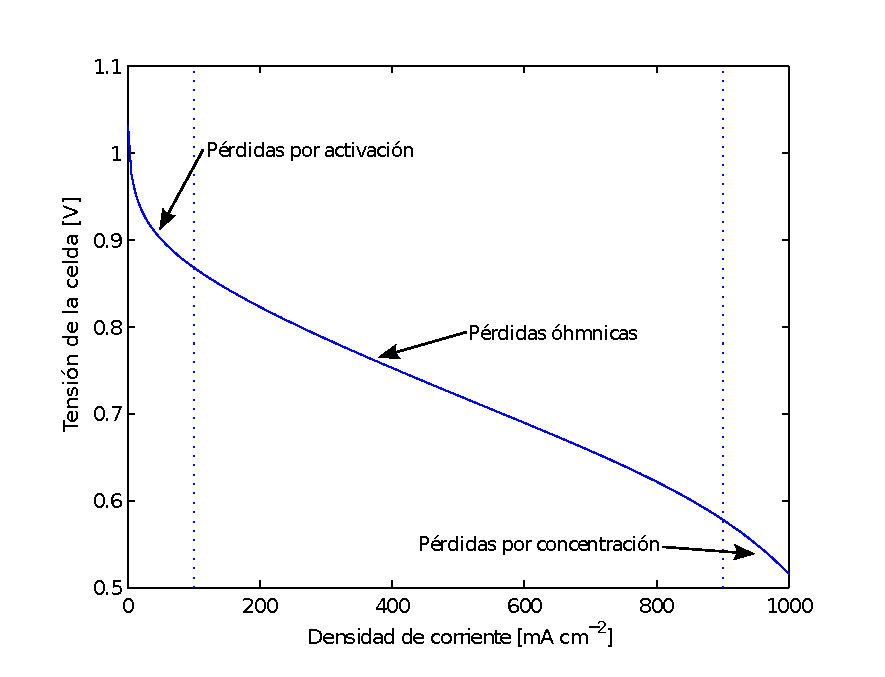
\includegraphics[width=10cm]{gfx/cacteristica_electrica_inf.eps}
 \caption{Característica típica de tensión-densidad de corriente.}
 \label{fig:caracteristica_electrica}
\end{figure}



\section{Comentarios}
Las celdas de combustible han sido presentadas y se han comentado varias de su principales cualidades. Entre ellas se han encontrado algunas
ventajas y otros inconvenientes.
El panorama brindado en éste capítulo ha servido como soporte teórico al trabajo desarrollado para la construcción del emulador de celdas de combustible
y permitirá proseguir al siguiente capítulo que se centra en las características eléctricas en los modelos adoptados para el diseño.
\end{comment}

%Capítulo 3

\chapter{Estudio de la calibración interna clásica}
\label{ch:classicalCalibration}
\lhead{\emph{Estudio de la calibración interna clásica}}
%----------------------------------------------------------------------------------------

En este capítulo se introduce el esquema de calibración clásico. Se busca:
\begin{itemize}
	\item Determinar el funcionamiento del método para introducir dicho comportamiento en el modelo de antena. 
	\item Determinar las virtudes y limitaciones del método para simular los distintos escenarios de fallas de la antena.
\end{itemize}


\section{Descripción del método}

Como fue introducido previamente, la antena se conecta a un transmisor y un receptor que es comandado desde la UCC y consta de
una serie de elementos que han sido identificados en el capitulo previo para su modelización matemática y algorítmica. Como 
pueden haber dispersiones en el comportamiento de cada componente dentro del lazo de calibración, se hace uso de la calibración
interna para compensarlas. 

Este método es utilizado para poder medir, detectar y corregir el mal funcionamiento de parte de la RFDN y, en particular, todas
las desviaciones se las atribuyen a los TRMs. Siendo estos, los actuadores que permiten compensar las desviaciones entre lo medido
y lo deseado. A su vez, también se puede detectar si uno de dichos módulos queda inhabilitado a causa que cierta parte de la
cadena de transmisión/recepción o dicho componente se destruyó.

Tal como se mencionó previamente, una de las principales limitaciones de la calibración interna clásica es que no puede
detectar variaciones, o medir, las partes pasivas del sistema que están fuera del lazo de calibración interna. Un ejemplo de
esto son los elementos radiantes de la figura \ref{fig:classic_cal_scheme} donde se puede observar que quedan fuera de los lazos
de calibración tanto en transmisión (línea punteada) como recepción (línea llena). Por otra parte no se puede detectar la
ganancia absoluta, debido a la ausencia de un blanco estándar de calibración \cite{Wang2010}.

En la figura \ref{fig:classic_cal_scheme} se muestra el esquema de calibración, en el cual se observan tres modos de
calibración. Cada uno posee distintos caminos, \textbf{P1} (línea punteada roja) caracteriza el camino de transmisión,
\textbf{P2} (línea llena azul) caracteriza el camino de recepción y \textbf{P3} caracteriza la unidad central de control (UCC).
\textbf{P3} es utilizado para corregir posibles variaciones en los pulsos \textbf{P1} y \textbf{P2} \cite{Makhoul2012}. Se puede
apreciar que, para este esquema en particular, tanto los elementos radiantes como sus cables de interconexión no forman parte de
lazos de calibración interna. En otras palabras, cualquier variación en el comportamiento de RF de los mismos, representados
por los parámetros S, no serán detectados al realizar dicha calibración.

Si el comportamiento del sistema depende de elementos que no están bajo control, sería un problema. En principio se podría
pensar en utilizar componentes fuera del lazo que se sabe que no van a variar en toda la vida útil del dispositivo. Como esto en
general no es viable, la solución a la que se suele recurrir es la caracterización en todas sus variables (temperatura,
frecuencia) de dichos elementos y al deseo de que esta caracterización perdure en el tiempo.

\begin{figure}[H]
 \centering
 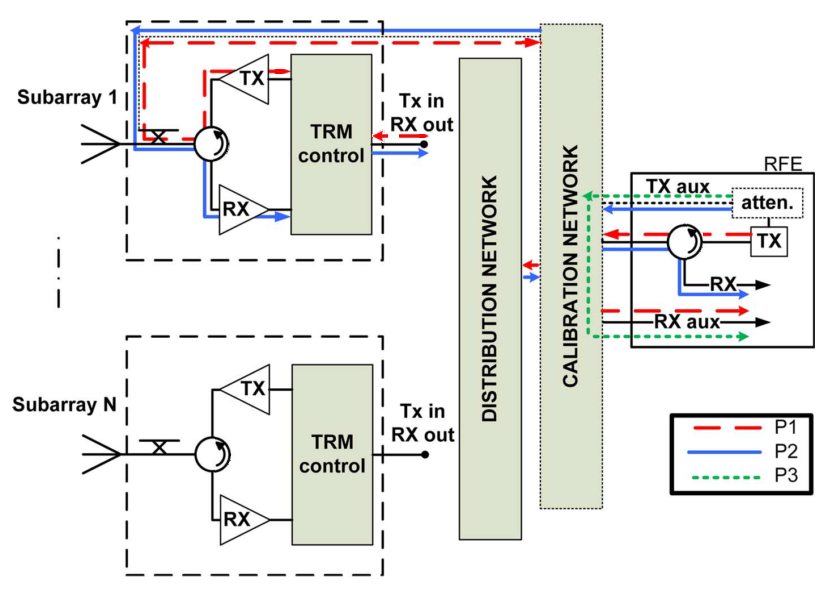
\includegraphics[width=10cm]{gfx/classic_cal_scheme.png}
 \caption{Esquema de calibración interna: camino de calibración de pulsos \textbf{P1} (Tx) en línea punteada, \textbf{P2} (Rx)
 en línea llena y \textbf{P3} (UCC) en verde \cite{Makhoul2012}.}
 \label{fig:classic_cal_scheme}
\end{figure}

Como ejemplos de sistemas que utilizaron dicho método, se puede nombrar al instrumento radar de los satélites E-ERS-1, SIR-C
\cite{Curlander1991}, terraSAR-X \cite{Schwerdt2005} y ENVISAT ASAR \cite{Loop}. La figura \ref{fig:calibrMethods} muestra los esquemas
de calibración de los primeros dos sistemas mencionados.

\begin{figure}[H]
	\centering
	\subfloat[instrumento radar del satélite E-ERS-1]{
		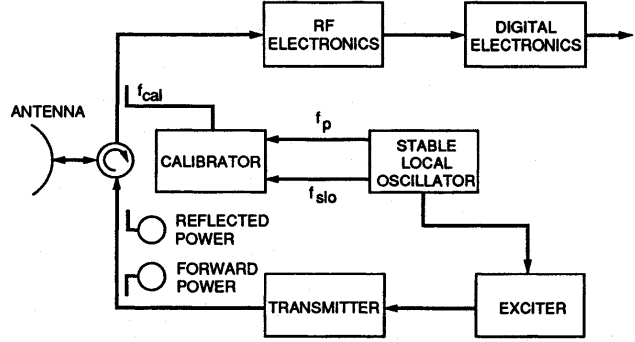
\includegraphics[width=7cm]{gfx/sirCalibration.png}}
 	\subfloat[instrumento radar del satélite SIR-C]{
		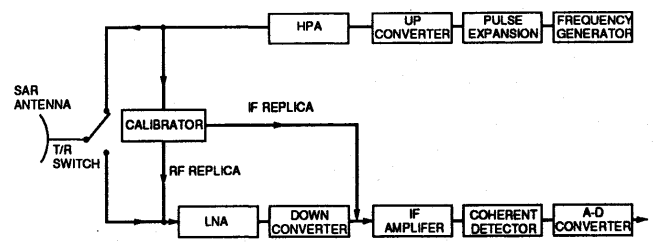
\includegraphics[width=7cm]{gfx/eersCalibration.png}}
	\caption{Esquemas de calibración interna del instrumento radar \cite{Curlander1991}.}
	\label{fig:calibrMethods}
\end{figure}


\subsection{Método} \label{ssc:classicalMethod}

No solo es necesaria la medición de la estabilidad del instrumento, sino que también se requiere obtener información del
comportamiento de los TRMs de forma individual, dado que el apuntamiento y la planitud del frente de onda de la señal dependen
de la ganancia y fase configurada de estos componentes. Por lo tanto, es necesario conocer el estado actual de los TRMs,
especialmente si se considera una posible degradación en el desempeño o mal funcionamiento de los mismos \cite{Br2007}.

Una estrategia para mediciones individuales de cada TRM requiere que el resto de dichos componentes estén apagados 
\cite{Br2007}. El problema de esta estrategia es que, al tener parte de la antena apagada, no resulta un método representativo
al modo de funcionamiento nominal (toda la antena operativa).

Para resolver este problema y calibrar todos los TRMs en simultáneo, al menos en transmisión o en recepción, se emiten
subsecuentes pulsos de calibración modificando los parámetros configurables que introducen los actuadores al sistema, en este
caso la fase introducida por los TRMs. De esta forma, se arma una codificación diferente para cada lazo de calibración de forma
tal que los distintos códigos sean ortogonales entre sí. Este algoritmo se llama PCC.

En esta tesis se utilizan los códigos walsh para codificar cada lazo de calibración \cite{Singhal2012}. En esta estrategia se
configura el desfase de cada TRM en para cada pulso de calibración en $\pm90^{\circ}$ con respecto a la fase que poseía la
antena en el momento de iniciar el proceso de calibración. Siguiendo una determinada secuencia $c_{mn}(t)$.

\begin{figure}
 \centering
 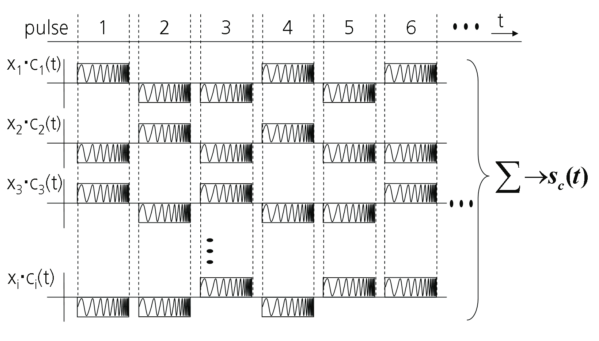
\includegraphics[width=8cm]{gfx/superposition_signals_classic.png}
 \caption{Superposición de señales de todos los TRMs. Cada señal tiene su propia secuencia de código aplicada entre pulsos
 \cite{Br2007}.}
 \label{fig:sup_sign_classic}
\end{figure}

La figura \ref{fig:sup_sign_classic} muestra la superposición de la señal de calibración con las distintas fases que adoptan
los $j$ TRMs de la antena en los $n$ pulsos requeridos para completar la codificación utilizada.

Por lo tanto, la fase de salida de cada TRM es la fase de la señal sumada a la configurada previamente a iniciar la
calibración, $\varphi_{mn}$, junto al desfase del código de $90^{\circ}$. Consecuentemente, la superposición de todas las
ganancias de los TRMs, $a_{mn}$, y fases, $\varphi_{mn}$, es obtenida en el puerto de recepción de la RFDN, $s_c(t)$ como se
muestra en la figura \ref{fig:sup_sign_classic}.

\begin{equation}
	s_c(t) = \sum_{m=0}^{M-1}\sum_{n=0}^{N-1}c_{mn}\cdot a_{mn}e^{j\varphi{mn}} + n_{mn}
\end{equation}

Donde $n_{mn}$ es el ruido inherente que hay en las mediciones de cada TRM. Para decodificar y obtener la ganancia
$\tilde{a}_{mn}$ y fase estimada $\tilde\varphi_{mn}$ de algún TRM, la señal compuesta $s_c$ es correlacionada con
la secuencia del módulo deseado. Con esta correlación, la modulación de la secuencia se elimina dando como resultado
la ganancia estimada.

\begin{equation}
\begin{aligned}
	\tilde{x}_{mn} &= s_c \otimes c^*_{mn} \\
	\tilde{x}_{mn} = \int s_c(t) &\cdot c^*_{mn}(t) dt = \tilde{a}_{mn}e^{j\tilde{\varphi}_{mn}} \\
\end{aligned}
\label{eq:classic_correlation}
\end{equation}

En general el código de calibración utilizado es el código walsh \cite{Singhal2012}. Dicho código deriva de las matrices de 
Hadamard (ver apéndice \ref{AppendixB}); dadas sus propiedades de ortogonalidad, cada código, o fila, es unívocamente 
distinguible del resto. Para minimizar la cantidad de mediciones, el largo del código ($l$) debe ser lo más corto posible. 
El número de TRMs de la antena es el determinante de la cota inferior.

\begin{equation}
	l = 2^i \ge N \cdot M
\end{equation}

Asumiendo $N$ la cantidad de filas y $M$ la cantidad de paneles, o columnas, que tiene el conjunto de antena, se utilizan tres
estrategias con este método de calibración para obtener distintos niveles de granularidad de mediciones a saber.

\begin{itemize}
	\item \textbf{Nivel módulo:} Este nivel es el que utiliza los códigos más largos, dado que se calibran todos los módulos que
		posee la antena en una polarización determinada ($l = 2^i \ge N \cdot M$).
	\item \textbf{Nivel panel:} En este nivel se utiliza el mismo código para todos los TRMs que son de un mismo panel,
		logrando así, decrecer el largo del código ($l = 2^i \ge M$).
	\item \textbf{Nivel fila:} En este nivel se utiliza el mismo código para todos los TRMs que son de una misma fila,
		logrando así, decrecer el largo del código ($l = 2^i \ge N$).
\end{itemize}

Este método a nivel panel y fila sirve para la caracterización del la configuración del apuntamiento de antena \cite{Br2007}.


\subsection{Limitaciones}

La calibración clásica se utiliza típicamente con el objeto de detectar componentes que funcionan mal, en particular los
TRM. Puesto que si un TRM presenta alguna falla en su funcionamiento como ser por ejemplo un amplificador que no responde, esto
se puede detectar en la calibración interna clásica mediante el lazo de calibración. Sin embargo, este esquema presenta varias
desventajas, descriptas en las siguientes secciones.


\subsubsection{Caracterización previa de los elementos de antena}

Para poder conocer la ganancia del lazo de transmisión o recepción es necesario conocer la potencia de la señal de
calibración, para sustraerla del resultado obtenido. El lazo de calibración donde se realiza esta medición es el que se
muestra en la imagen \ref{fig:classic_cal_scheme}, llamado \textbf{P3}. En esta medición no se puede determinar cuanto atenúa
el lazo, por lo tanto se opta por caracterizar en tierra dichos componentes para las frecuencias y temperaturas de trabajo.

Tener que recurrir a las caracterizaciones a los componentes de la antena presentan las siguientes desventajas: 

\begin{itemize}
	\item Costo de materiales: Componentes caracterizados en temperatura pueden costar varias veces el precio de un componente sin
		caracterizar. Esto es debido a que los ensayos de caracterización térmicos son costosos. También lo es el equipamiento para
		realizar las características en frecuencia y muchas veces son rentados por las compañías ante la imposibilidad de comprarlos.
	\item Costo de recursos: La campaña de caracterización no solo puede durar meses sino que también requiere una dedicación
		casi total de equipos de gente a dicha actividad, implicando un gasto de dinero muy importante. En algunos proyectos donde hay
		fechas preacordadas que respetar, pueden determinar que dichos costos sean inviables.
	\item Comportamiento de materiales a lo largo del tiempo: Como el material envejece, cambia sus propiedades, por lo tanto las mediciones
		realizadas en la campaña de caracterización dejan de tener validez.
\end{itemize}


\subsubsection{Complejidad del hardware de la antena}

Como se calibra solo una parte de la antena por vez, transmisión o recepción en una u otra polarización (H o V), es necesario
que el lazo de calibración esté compuesto por la parte de la antena a calibrar junto a hardware dedicado (cables e interruptores) a
esta tarea. De esta forma, se añaden las siguientes desventajas:

\begin{itemize}
	\item Incremento en complejidad de HW: El HW de la antena resulta más complejo por el agregado de componentes dedicados a la
		calibración.
	\item Caracterizaciones extra: Se debe caracterizar el HW dedicado a la calibración, para restar el desfase y atenuación
		agregado en el momento de realizar la calibración.
	\item Acoplamiento: Como hay hardware agregado, se debe tomar recaudo ante el incremento de los posibles acoplamientos entre
		componentes.	
\end{itemize}


\subsubsection{Susceptibilidad ante inestabilidad del generador}

Este método es susceptible a las variaciones de fase y potencia del generador entre pulsos de calibración. Por lo tanto, es de
vital importancia contar con un generador que sea estable.


\subsubsection{Sistema incompleto}

Como hay componentes que están fuera de los lazos de calibración, con el método nunca se puede determinar de forma totalmente
correcta la ganancia de la antena en cualquiera de sus modos.


\subsubsection{Optimización en la longitud de código del PCC}

A la hora de elegir la longitud del código Walsh, es importante que siempre haya un elemento radiante virtual en la antena para
evitar la primer columna de la matriz de códigos. En caso contrario el primer TRM siempre tendrá un error en la estimación de
su ganancia \cite{Wang2010}.


\subsubsection{Pérdida de ortogonalidad en el código utilizado por comportamiento de desfasadores}

Si el desfasador no tiene un comportamiento exactamente igual al configurado a la hora de realizar la calibración, los códigos
walsh pierden ortogonalidad y, por ende, se logra obtener una mala estimación de los valores de ganancia de la antena.


\subsubsection{Compensación de temperatura en elementos}

Se debe mantener la temperatura de los elementos en los valores caracterizados para garantizar que las calibraciones sirven.


\subsubsection{Dependencia del modelo y análisis térmico}

Es completamente dependiente del modelo y análisis térmico. Por ejemplo, se asume que el comportamiento de los elementos
radiantes de la antena no varían con la temperatura.

\section{Conclusiones}

En este capítulo se introdujo tanto el modelo matemático de la calibración interna clásica como su forma de operar. A su vez,
se brindaron ejemplos de satélites en donde su sistema de radar utiliza este método.

Se llegó a la conclusión que este método sirve para poder determinar que un TRM funcione correctamente, pero si se lo desea
utilizar para otro objetivo, por ejemplo el de corregir el diagrama de radiación de la señal transmitida, hay que tener recaudos
en la cantidad de inconvenientes que trae aparejado. Por ejemplo, que no abarca la totalidad del sistema, los costos en tiempo y
recursos asociados a la campaña de caracterización y que se tenga fé de que con el envejecimiento de los componentes, dichas
caracterizaciones van a continuar sirviendo.


\chapter{Calibración utilizando acoplamientos mútuos}
\label{ch:convertidores}
\lhead{\emph{Calibración utilizando acoplamientos mútuos}}
%\lhead{\emph{Celdas de combustible}}

\section{Calibración utilizando acoplamientos mútuos}

Una de las grandes ventajas de este método frente al método anterior es que no requiere hardware extra, logrando así 
disminuir la complejidad de la antena, de esta forma se puede construir de una forma más compacta.

Tomando como $M$ la cantidad de filas de módulos radiantes por panel y $N$ la cantidad de paneles, las tres modalidades de 
este método son:

\begin{itemize}
	\item \textbf{Modo completo:} En esta modalidad no solo se estima la ganancia en transmisión y recepción en ambas 
		polarizaciones (H y V), sino que también se determina la planitud de la antena. La cantidad de ecuaciones necesarias es 
		de $MN(MN + 7)/2$.
	\item \textbf{Modo rápido:} En esta modalidad se estima la ganancia en transmisión y recepción em ambas polarizaciones
		(H y V) utilizando el valor guardado de la planitud de la antena calculado previamente. La cantidad de ecuaciones necesarias
		es de $4MN$.
	\item \textbf{Modo planitud ideal:} Esta modalidad es igual al modo rápido, asuminedo que la antena es perfectamente plana. 
		La cantidad de ecuaciones necesarias es de $4MN$.
\end{itemize}

El modo planitud ideal cuenta con otra limitación que, para poder ser utilizado en una antena de cualquier topología utiliza 
lazos de calibración de tal forma que el acoplamiento mutuo queda eliminado. Para esto hay dos estrategias, la primera transmite 
con un RM y recibe de forma consecutiva con otros RMs equiespaciados al de transmisión para luego restar ambos caminos. La 
segunda, transmite de forma consecutiva desde los RMs equiespaciados y recibe con un único RM central, la imagen 

\todo{crear la imagen para esa cosa}
\begin{figure}[H]
 \centering
	\subfloat[]{	
		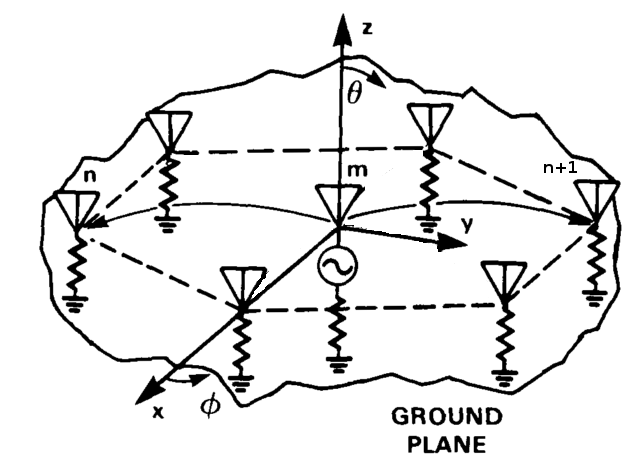
\includegraphics[width=5cm]{gfx/mutualRxCal.png}}
	\subfloat[]{	
		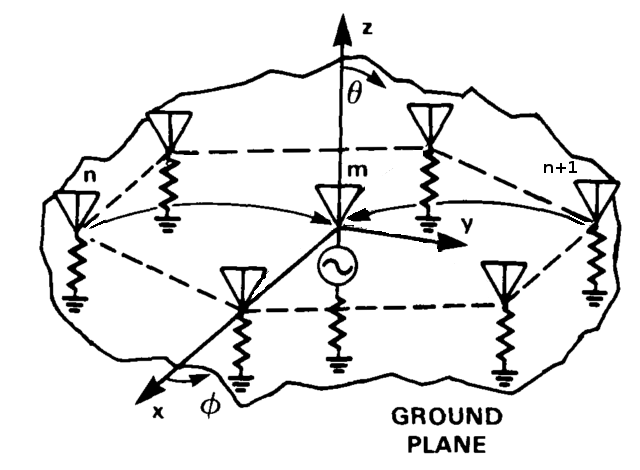
\includegraphics[width=5cm]{gfx/mutualTxCal.png}}
 \caption{estrategia de planitud ideal. (a) Calibra lazos de recepción, (b) Calibra lazos de transmisión}
 \label{fig:ideal_strategy}
\end{figure}




Aprovechando la realidad que las variaciones mecánicas son lentas frente a las variaciones eléctricas de los componentes,
no es necesario correr el método de calibración en su máxima caracterización dado que requiere demasiada cantidad de 
mediciones para determinar la planitud de la antena.


Referencias a utilizar: 
Shipley2000
Aumann1989
Gao2001 (este no esta tan copado, son puras formulas)
a calibration technique for active phased array antennas (no lo agregue aun a la bibliografia, je)
Practical faliure compensation in active phased antennas (ni lo lei, pero muy interesante que hacer para compensar algo quemado)


Modem phased arrays typically have excellent performance, but still must occasionally undergo phase and amplitude calibration in order to realize their full performance potential. This must be done at least upon completion of antenna fabrication. At the factory, this initial calibration is usually done on a near- field scanning or compact range, and is typically very time consuming. Re-calibration after operational deployment is also required to maintain peak Performance levels, but is typically not done, due to practical difficulties. Re-calibration is also needed if repairs or changes are made in the antenna.
TSC


\todo{poner en algun lado que se sugiere para medir la fase de medir en un unico punto lo que defasa la antena punta a punta una unica vez y se lo carga al metodo}
\todo[inline]{esto es texto viejo... el capitulo 5 tiene lo mismo}
Una antena se calibra buscando que no solo todos los caminos de recepción atenúen y defasen exactamente lo mismo, sino que 
también sea un valor conocido. Para transmisión se busca lo mismo, con la salvedad que se puede modificar la fase de la 
señal que se emite en algunos RMs para modificar el lugar de apuntamiento de la antena.

Hay distintos factores que hacen que los componentes dejen de comportarse de forma nominal, por ejemplo se puede nombrar el
cambio de temperatura, el mero envejecimiento de los componentes al pasar el tiempo, que un mero cable se haya doblado más
de la cuenta, interferencias electromagnéticas, radiadas o conducidas, o entre distintos componentes, etc. 

Es importante que un patrón de antena posea los lóbulos secundarios lo más chicos posibles con respecto al lóbulo principal,
que el lóbulo principal sea lo más angosto posible, con esto se aumenta la resolución espacial. Un factor que ocurre es el 
de los targets ficticios.\todo{no se como se elimina}


\todo{poner que factores hacen que cambie la ganancia de los componentes para calibrar la antena}
\todo{poner que ocurre con el antnena pattern si no está correctamente calibrada, altura de lóbulos secundarios, ancho 
de lóbulo principal, pico del lóbulo principal, etc}

Para poder calibrar esta antena polarimétrica haciendo uso de los acoplamientos mutuos, se cuenta con el uso de 
cuadrados mínimos. La idea es realizar lazos de calibración transmitiendo en una polarización y recibiendo en la
otra a la vez. Para esto, es necesario que no solo se pueda configurar algunos RMs em modo $T_x$ y otros en modo $R_x$ en 
distintas polarizaciones, sino también poder configurar los módulos que no forman parte de dicho lazo en modo alta 
impedancia (en este modo el módulo no transmite ni recibe nada, evitando así la inyección de ruido y señal en zonas 
indeseadas de la antena). 

Tomando como caso una antena rectangular de $M x N$ módulos radiantes y asumiendo que solo se transmite y recibe de a un 
RM por lazo de calibración, a priori, se dispone de un máximo de $(MN)^2$ ecuaciones. La cantidad de incógnitas de todos
los caminos de la RFDN, tanto transmisión como recepción en ambas polarizaciones (H y V), son $4MN$. A su vez, en el 
apéndice \ref{AppendixA} se realiza el cálculo de la cantidad de acoplamientos mutuos que posee una antena polarimétrica,
particularmente, la ecuación \ref{eq:amountMutCoupling} muestra la cantidad de incógnitas, que, para este caso, resulta 
ser de $MN(MN-1)/2$. Totalizando en $MN(MN + 7)/2$ incógnitas.

Para que el sistema tenga solución, la cantidad de ecuaciones debe ser mayor que la de incógnitas. Esta restricción solo 
se cumple si se calibra toda la antena en un solo paso (Tx y Rx en ambas polarizaciones) porque es el único caso en que 
cada acoplamiento mútuo aparezca más de una única vez. En caso contrario, habrían siempre más incógnitas que ecuaciones.

\todo{tener en cuenta que por ahora el requerimiento es que la antena sea totalmente plana}




\begin{comment}

Los convertidores conmutados son equipos de potencia utilizados para proveer una tensión regulada a partir
de una fuente de de energía eléctrica. Su característica principal es su gran eficiencia, comparados con otros
sistemas de conversión, gracias al mecanismo de conmutación en que están basados.

Existen varias configuraciones de circuitos de convertidores y en general se apoyan en tres topologías básicas cuya característica
les permite elevar o reducir la tensión, o bien realizar ambas. Estas configuraciones pueden ser modificadas
para adicionar algunos atributos como aislamiento eléctrico, múltiples niveles de tensión o la simplificación del accionamiento de las llaves electrónicas.

El principio operacional de los convertidores consiste en cambiar la estructura del circuito mediante
la activación de las llaves electrónicas, provocando un cambio en el comportamiento general del sistema.

Una de sus principales características es el control que se adopta en la apertura y cierre de las llaves electrónicas.
En general las señales de conmutación que ordenan su apertura o cierre, provienen de pulsos de ancho modulado (PWM)
cuya operación se controla a través de alguna referencia interna al dispositivo que las acciona.

Ciertos parámetros definen la operación de los convertidores de potencia, entre los más importantes se encuentran
la frecuencia de conmutación y el ciclo de trabajo correspondiente al tiempo de apertura de la llave activa, denotada por $D$.

La operación de los convertidores trabajando en régimen permanente se distingue en dos modos de operación que tienen
en cuenta el paso de corriente a través del inductor. Estos modos son los de \emph{conducción continua} y \emph{conducción discontinua}:
en el primero la corriente no se interrumpe y en el otro existe un intervalo en que se mantiene nula.

El rol de estos convertidores es de especial importancia para cualquier aplicación de las pilas de celdas de combustible 
debido a los cambios que sufre la tensión entregada ante cambios de carga, como se mostró en el cap. \ref{ch:modelo}.

En un SGH, estos convertidores son requeridos por tratarse de los dispositivos a través de los que se adaptan
los módulos de generación a la línea de distribución de energía. Para el proyecto de la construcción del SGH abordado se realizó
la construcción de una etapa de potencia para adaptar cierta pila de combustible al bus de tensión continua del sistema. Este dispositivo
fue hecho de modo que pudiera elevar la tensión entregada por la celda al nivel del la línea de distribución. Dado que el convertidor
cuenta con las especificaciones de diseño para operar con celdas de combustible fue elegido como soporte físico para el desarrollo del emulador.

Para la operación del emulador es necesario que el dispositivo de potencia pueda reducir la tensión, que es el comportamiento
general de las celdas de combustible al ser cargadas con cierta corriente. Por tanto se requirieron ciertos ajustes a nivel de \emph{software} 
y \emph{hardware} al convertidor ya diseñado para que tenga la capacidad de reducir la tensión en lugar de aumentarla. Las modificaciones 
realizadas sobre el elevador serán explicadas hacia el final del capítulo mientras que el control implementado será explicado en el cap. \ref{ch:control}.

Para la realización de los análisis siguientes se establecen las siguientes aproximaciones, que permiten simplificar
los cálculos con suficiente precisión:
\begin{itemize}
 \item El capacitor del filtro de tensión de salida es suficientemente grande para que se desprecie la variación
 de tensión a la salida.
 \item El inductor es suficientemente grande para que la corriente pueda ser considerada por tramos lineales.
 Este hecho permite establecer la siguiente aproximación:
 \begin{equation}
  \frac{di_L}{dt}\approx \frac{\Delta i_L}{\Delta t}\Rightarrow \Delta i_L=\frac{di_L}{dt}\Delta t
  \label{eq:aprox_corriente}
 \end{equation}
 Y la derivada representa la pendiente de la corriente en el subintervalo correspondiente.
 \item La corriente no sufre grandes variaciones debido a la presencia de elementos parásitos.
\end{itemize}

Este capítulo presenta las características generales de los convertidores utilizados y los parámetros utilizados para su control. 
El análisis se comienza por el dispositivo elevador original debido a que fue el soporte inicial. Luego se explicarán las características
técnicas particulares de cada convertidor utilizado.

A continuación se dará un explicación más detallada de los convertidores utilizados, su funcionamiento en régimen permanente en ambas
condiciones de conducción y el modelo dinámico que será utilizado para diseñar los controladores implementados.

\section{Convertidor elevador}
Este sistema de potencia, como indica su nombre, es usado para llevar la tensión de entrada a un nivel mayor. La
fig. \ref{fig:elevador} muestra un diagrama esquemático del circuito utilizado para la construcción de la etapa de potencia del SGH.
En ella se distingue la particularidad de la capacidad bidireccional de corriente que le confiere el uso de dos llaves de conmutación
en lugar de una, como sería en el caso más básico. Esta característica permite que el convertidor sea capaz de devolver potencia a la fuente y además
le da flexibilidad al modelo, cuya cualidad se aprovechó para cambiar la topología sin realizar mayores modificaciones.
Para que ello sea posible, el proceso de fabricación que se realiza para obtener las llaves colocadas en el equipo utilizado implica 
la formación de una juntura PN entre los terminales de \emph{drain} y \emph{source}, lo que permite que ambas llaves conduzcan en ambos
sentidos, ya sea con la corriente pasando a través del canal del transistor (si se encuentra activo) en un sentido o con la corriente pasando a través del
diodo mencionado en el otro sentido.

\begin{figure}[H]
 \centering
 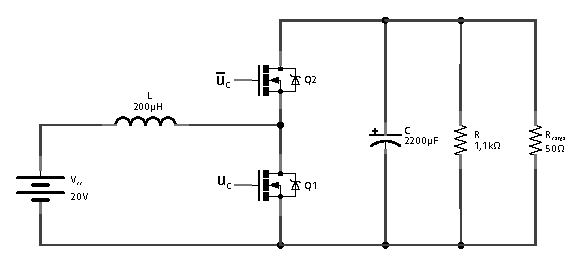
\includegraphics[width=10cm]{gfx/elevador.eps}
 \caption{Topología de un convertidor elevador de conducción bidireccional}
 \label{fig:elevador}
\end{figure}

\subsection{Operación en estado estacionario}
\label{sub:elevador_estacionario}
Una vez energizado y los transitorios extinguidos pueden analizarse las curvas eléctricas resultantes para obtener información acerca
de los parámetros de funcionamiento del convertidor y encontrar relaciones que serán útiles para el diseño del control. Esto puede hacerse 
cuando el convertidor opera en cualquiera de sus modos de funcionamiento.

\subsubsection{Modo de conducción continua}
Se procede a realizar una análisis del comportamiento del convertidor operando en modo de conducción continua (MCC). 
La fig. \ref{fig:elevador_CC} muestra las curvas genéricas de un convertidor utilizado funcionando en régimen permanente.

\begin{figure}
 \centering
 \subfloat[Tensión de inductor]{\label{fig:tension_inductor_elevador_MCC}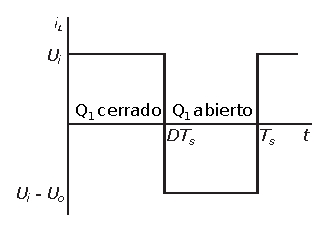
\includegraphics[width=5cm]{gfx/tension_inductor_elevador_MCC.eps}} \quad
 \subfloat[Corriente de diodo]{\label{fig:corriente_diodo_elevador_MCC}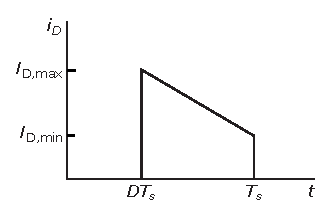
\includegraphics[width=5cm]{gfx/corriente_diodo_elevador_MCC.eps}} \\
 \subfloat[Corriente de inductor]{\label{fig:corriente_inductor_elevador_MCC}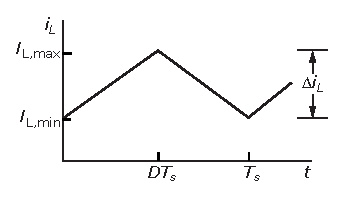
\includegraphics[width=5cm]{gfx/corriente_inductor_elevador_MCC.eps}} \quad
 \subfloat[Corriente de capacitor]{\label{fig:corriente_capacitor_elevador_MCC}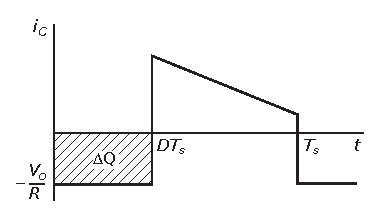
\includegraphics[width=5cm]{gfx/corriente_capacitor_elevador_MCC.eps}}
 \caption{Curvas de estado estacionario para el elevador operando en MCC}
 \label{fig:elevador_CC}
\end{figure}

Utilizando las curvas anteriores y conceptos elementales de la teoría de circuitos pueden obtenerse las relaciones que definen al funcionamiento
del elevador. El análisis realizado aquí considera también la presencia de algunos de los elementos parásitos que corresponden a las resistencias
equivalentes en serie del inductor, la llave y el capacitor (ESR), ya que constituyen los elementos no deseados de mayor peso al provocar
una reducción del desempeño general del convertidor.

La relación de conversión se obtiene analizando la integral de la tensión del inductor en un período, ya que el valor medio en estado estacionario es nulo
y se igualan las áreas correspondientes al tiempo de cada estado de las llaves. Este análisis se realiza a continuación despreciando el efecto de elementos parásitos,
$$ U_iD+(U_i-U_o)(1-D)=0 $$
Reagrupando queda,
\begin{equation}
 \frac{U_o}{U_i}=\frac{1}{1-D}
 \label{eq:relacion_elevador}
\end{equation}
Y haciendo $P_o=P_i$
\begin{equation}
 \frac{I_o}{I_i}=1-D
 \label{eq:relacion_corriente_elevador}
\end{equation}
Si se consideran las ESR se obtiene,
$$ (U_i-I_Lr)D+(U_i-I_Lr-U_o)(1-D)=0 $$
Para el caso de la tensión en el inductor,
\begin{equation}
 \frac{U_o}{U_i}=\frac{1-D}{(1-D)^2+\frac{r}{R}}
 \label{eq:relacion_elevador_completa}
\end{equation}
En la eq. (\ref{eq:relacion_elevador_completa} aparecen los parámetros de Resistencia de carga $R$ y la ESR, $r$.
A partir de la última ecuación se puede obtener la eficiencia del convertidor para distintas cargas haciendo el cociente entre la potencia
de salida y la de entrada usando (\ref{eq:relacion_corriente_elevador}) y (\ref{eq:relacion_elevador_completa}),
\begin{equation}
 \eta=\frac{P_o}{P_i}=\frac{(1-D)^2}{(1-D)^2+\frac{r}{R}}
 \label{eq:eficiencia_elevador}
\end{equation}
Es necesario aclarar que para llegar a estas ecuaciones se han realizado ciertas aproximaciones, sin embargo se consideran los efectos de las
pérdidas más importantes describiendo apropiadamente la operación del convertidor. En las figuras 
fig. \ref{fig:relacion_elevador} y \ref{fig:eficiencia_elevador} se muestran las curvas resultantes de los análisis anteriores.
\begin{figure}[H]
 \centering
 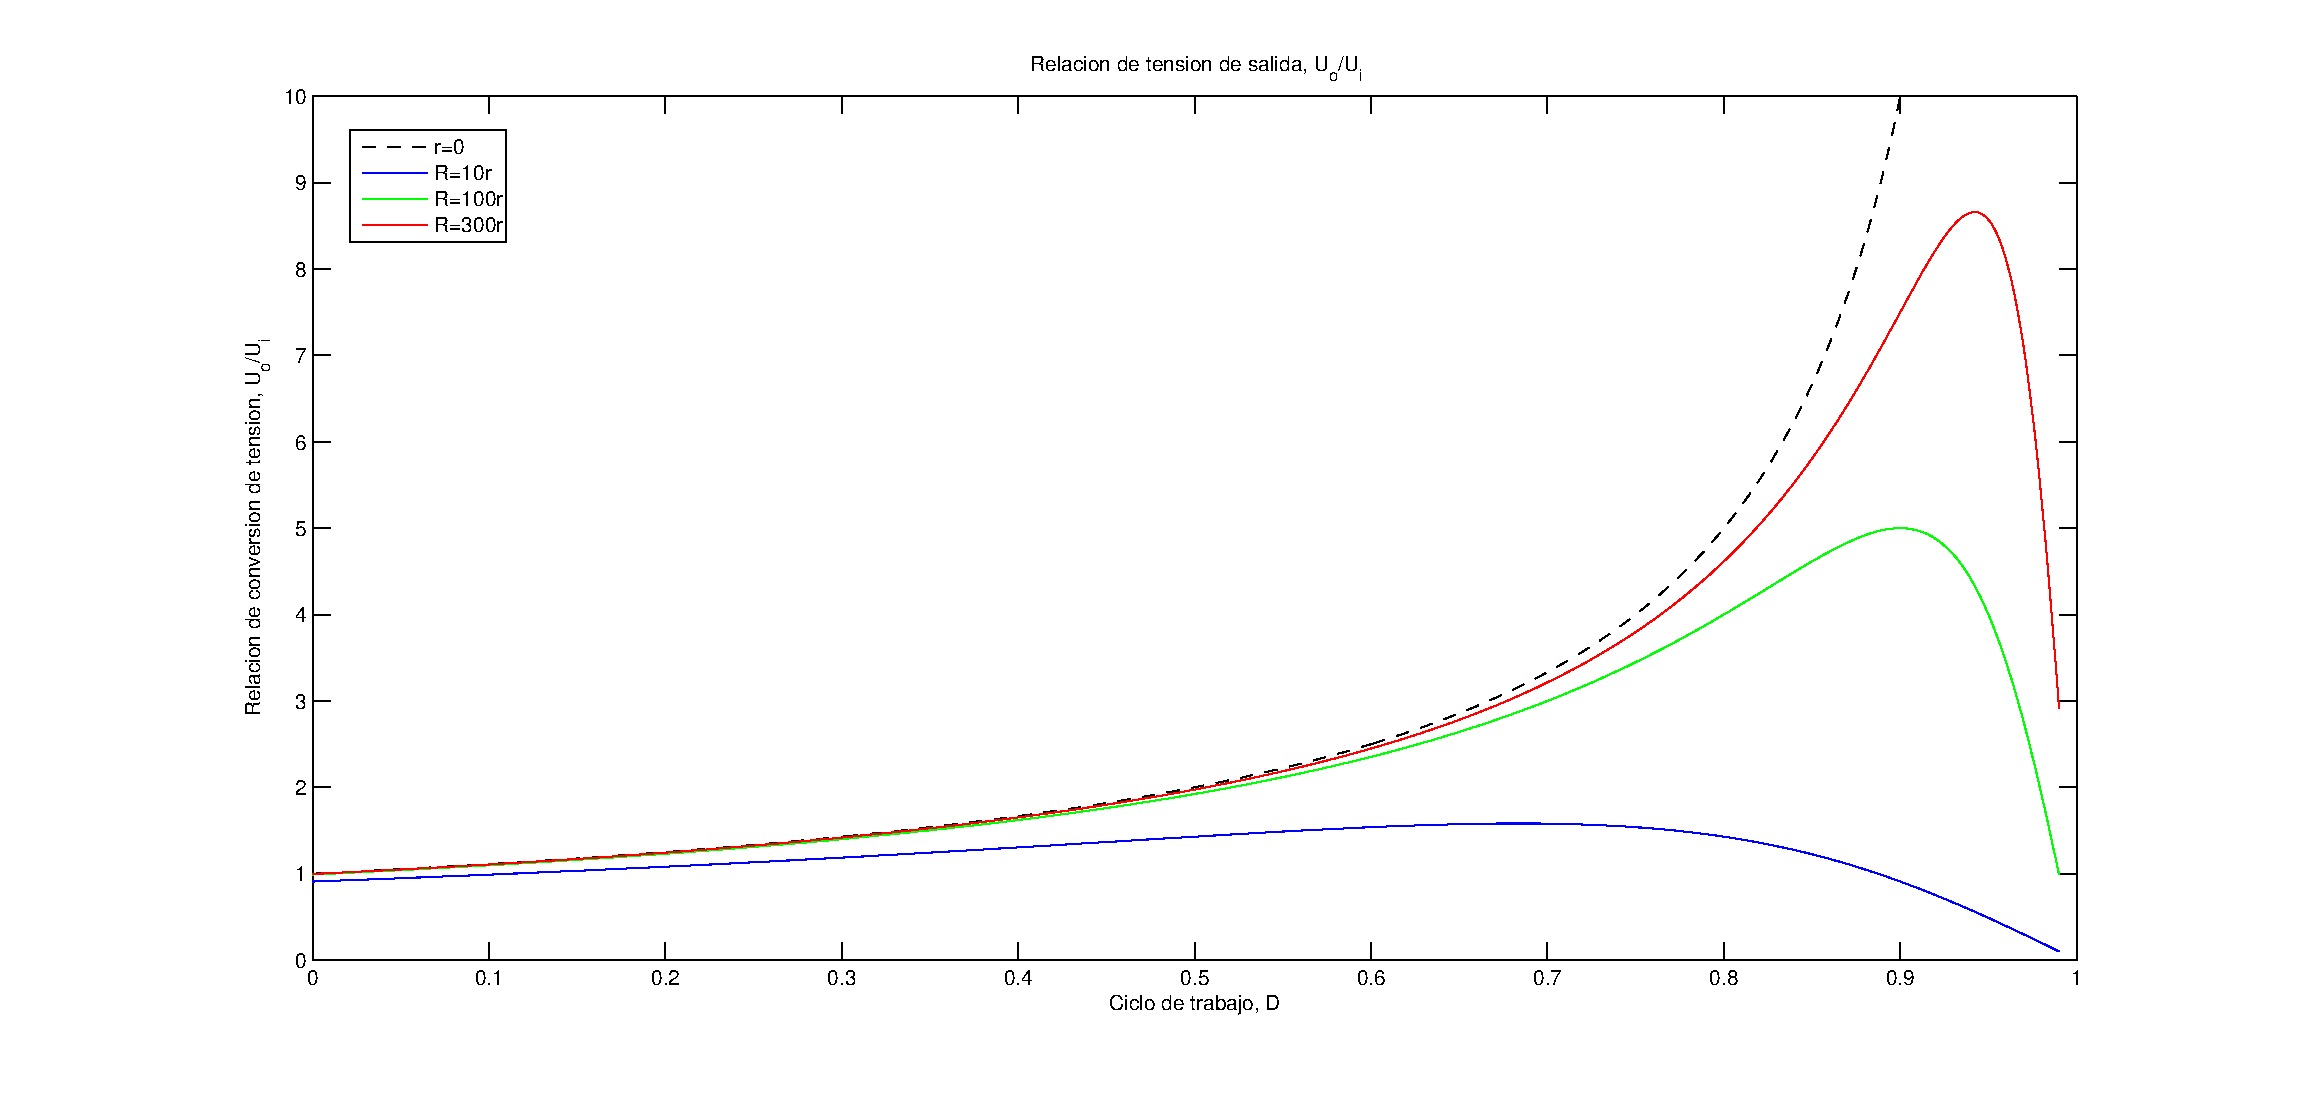
\includegraphics[width=12cm]{gfx/relacion_elevador.eps}
 \caption{Relaciones de tensión del convertidor elevador con diferentes cargas.}
 \label{fig:relacion_elevador}
\end{figure}
\begin{figure}[H]
 \centering
 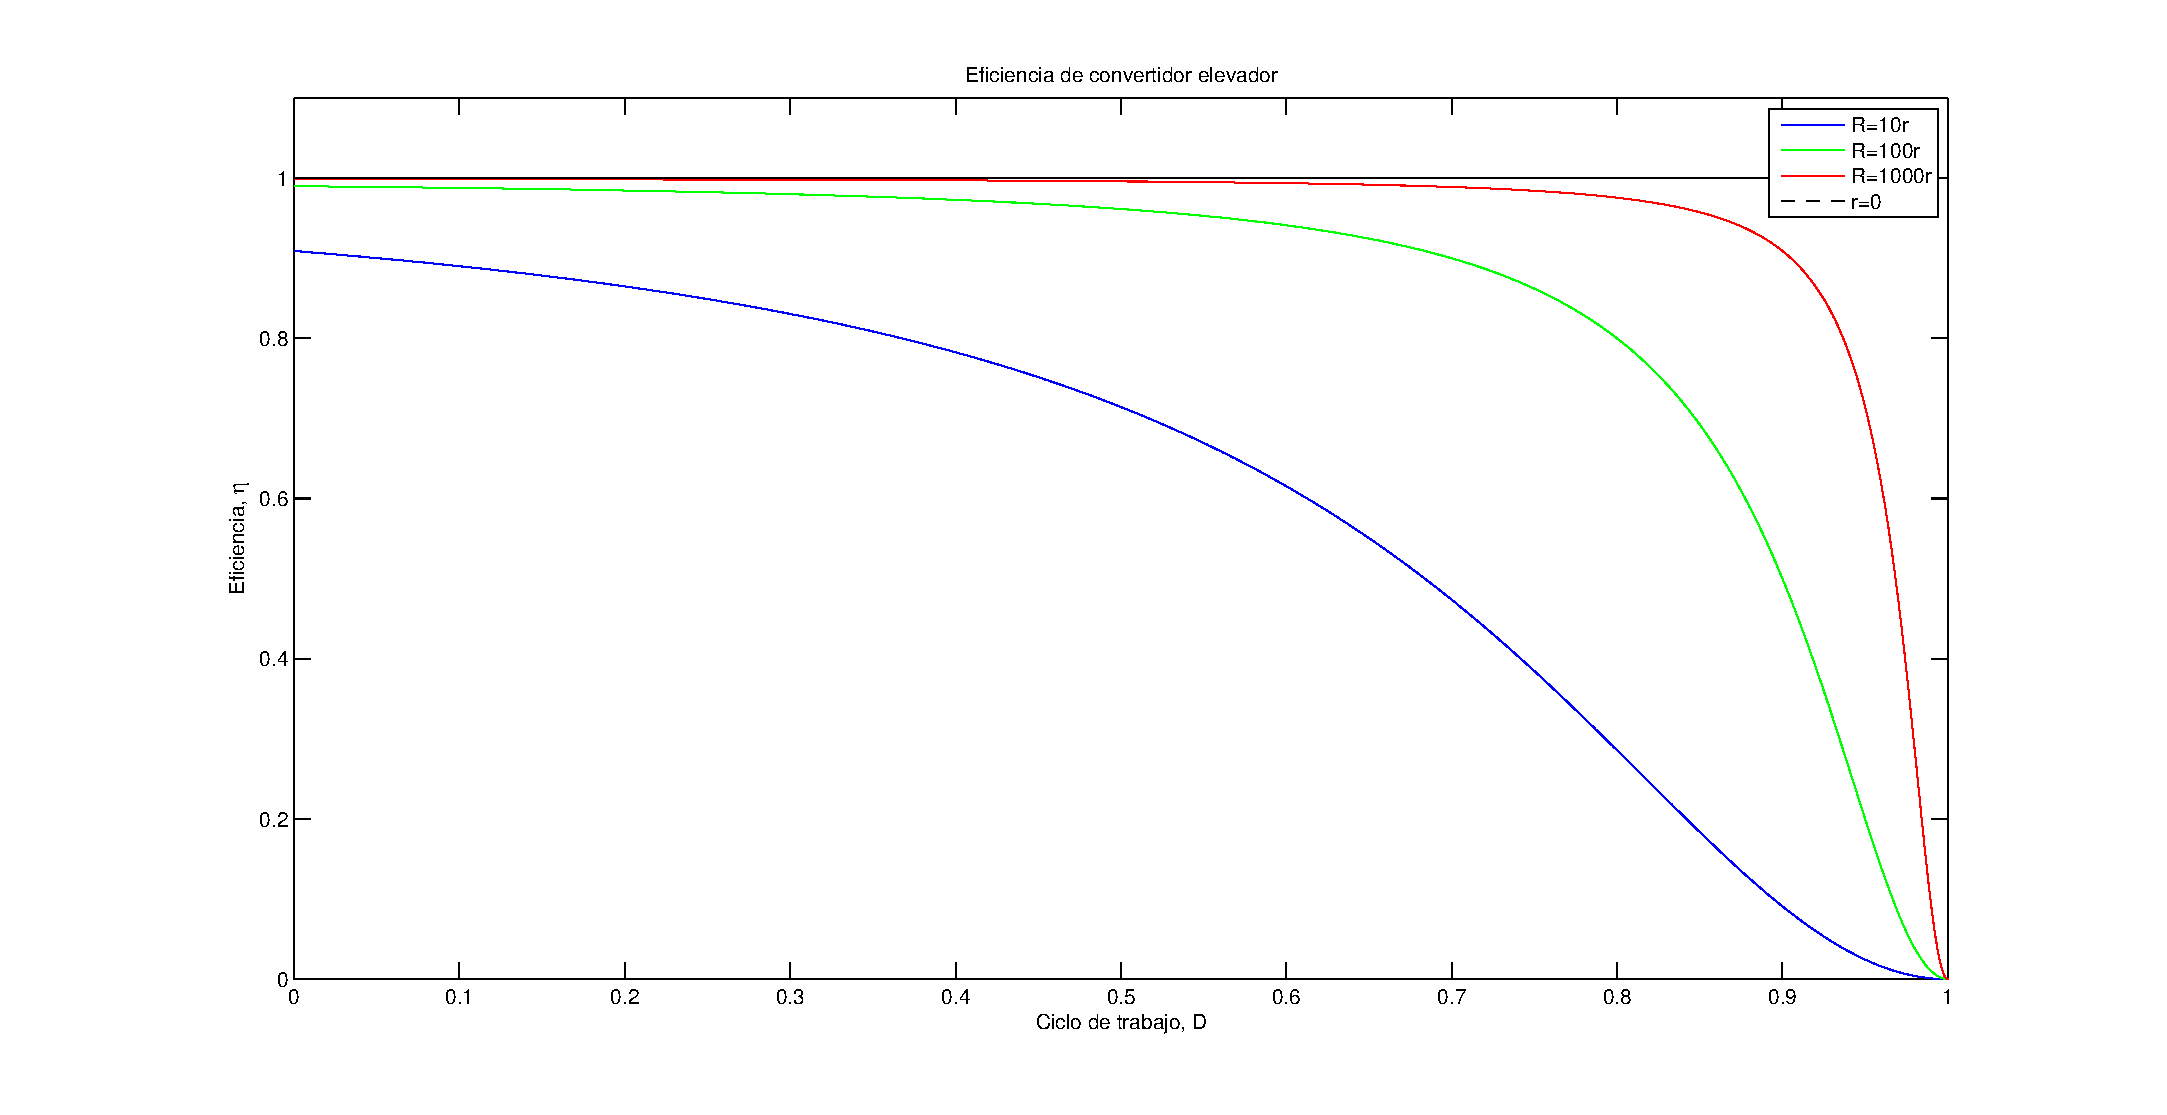
\includegraphics[width=12cm]{gfx/eficiencia_elevador.eps}
 \caption{Eficiencia del convertidor elevador a diferentes cargas.}
 \label{fig:eficiencia_elevador}
\end{figure}
Como el análisis se hace en estado estacionario si se examina la corriente que atraviesa el inductor usando la (\ref{eq:aprox_corriente})
la variación de la corriente es la misma tanto para la llave abierta como cerrada y resulta,
$$\frac{\Delta i_{L,cerrada}}{\Delta t}=\frac{\Delta i_{L,abierta}}{\Delta t}$$
\begin{subequations}
  \begin{equation}
   \Delta i_{L,cerrada}=\frac{U_i}{L}DT_s
  \end{equation}
  \begin{equation}
   \Delta i_{L,abierta}=\frac{U_i-U_o}{L}(1-D)T_s
  \end{equation}
\end{subequations}
A partir la fig. \ref{fig:elevador_CC} puede establecerse un límite entre los dos modos de operación MCC y MCD (modo de conducción discontinua).
Si se observa que al reducir la carga y con ella la corriente media a la salida del convertidor, también disminuye la corriente que atraviesa
el inductor, hay un punto en que $i_L$ se hace $0$. Teniendo en cuenta que la forma de la señal de corriente a través del inductor se aproxima
por una onda triangular se llega al siguiente resultado:
\begin{subequations}
 \begin{equation}
  \bar{i}_{L,min}=\frac{1}{2}\hat{i}_L
 \end{equation}
 \begin{equation}
  \bar{i}_{L,min}=\frac{1}{2}\frac{U_iDT_s}{L}
 \end{equation}
 \begin{equation}
  \bar{i}_{L,min}=\frac{1}{2}\frac{U_oD(1-D)T_s}{L}
 \end{equation}
\end{subequations}
Resulta útil expresar este límite en función de la corriente de carga, puesto que la tensión de salida se pretende mantener constante.
\begin{equation}
 \bar{i}_{o,min}=\frac{U_oT_s}{2L}D(1-D)^2
 \label{eq:limite_corriente_elevador}
\end{equation}
Al inicio del análisis se asumió que el capacitor del filtro de salida era suficientemente grande como para que la variación en la tensión de salida sea despreciable.
Aunque esta aproximación es válida para realizar los cálculos previos, se encuentra presente un pequeño rizado. Si se considera que en la práctica el
capacitor tiene capacidad finita y además posee una resistencia serie parásita (ESR) sobre la cual puede producirse una caída de tensión
puede hallarse una aproximación del valor del rizado de la tensión de salida. Esta variación se puede computar a partir de la variación en la carga del mismo y usando
la ley de ohm, respectivamente. 
Estos efectos pueden sumarse para considerar un caso pesimista del cálculo de la variación de tensión de salida,
$$\Delta U_o < \Delta U_{o,C} + \Delta U_{o,ESR} $$
Que establece una cota a partir de la suma de la variación provocada por la capacidad finita y la presencia de la resistencia parásita.

Para obtener la variación debido a la capacidad se estudia la corriente que atraviesa el capacitor,
$$ i_C=i_L-i_o $$
Para ello se examina la fig. \ref{fig:corriente_capacitor_elevador_MCC} y entonces si la corriente es positiva el capacitor se está cargando, en contraste si es
negativa, ocurre lo contrario. Partiendo de las definiciones de capacidad,
$$ \Delta U_{o,C}=\frac{\Delta Q}{C} $$
La variación de carga se obtiene al aplicar reglas geométricas al área sombreada de la fig. \ref{fig:corriente_capacitor_elevador_MCC}, asumiendo que 
$ I_o < i_{L,min}$,
$$ \Delta Q=I_o DT_s=\frac{U_o}{R}DT $$
Sustituyendo en la expresión anterior se tiene,
$$\Delta U_{o,C}=\frac{U_o DT}{RC}$$
En términos relativos,
\begin{equation}
 \frac{\Delta U_{o,C}}{U_o}=\frac{DT}{RC}
\end{equation}
Para obtener la caída debido a la ESR, simplemente se aplica la ley de ohm usando los valores de resistencia especificados por el fabricante y la variación de
corriente a través del capacitor.
\begin{equation}
 \Delta U_{o,ESR} = \Delta i_C r_C
\end{equation}
Hay que remarcar que muchas veces la caída de tensión debida a la resistencia parásita puede ser mucho mayor que la debida a la capacidad y por ello resulta muy importante
que se utilicen capacitores cuya ESR sea suficientemente baja para no degradar el desempeño del convertidor.

\subsubsection{Exigencias eléctricas en estado estacionario para MCC}

Es muy importante que no se sobrepasen los límites eléctricos para los cuales fueron fabricados los componentes que forman parte del convertidor para no
dañar los componentes. Si se inspeccionan las curvas de estado estacionario, se pueden encontrar las exigencias a las que serán sometidos. 
En el cuadro \ref{tab:exigencias_elevador} se encuentran las solicitaciones eléctricas de interés para cada componente.
\begin{table}[H]
  \centering
  \begin{tabular}{|c|c|c|c|c|}
  \hline 
  Comp. 	& $T_{1}$ & $T_{2}$ & $L$ & $C$\tabularnewline
  \hline 
  \hline 
  $U_{max}$	& $U_{o}$ & $U_{o}$ & $U_{o}-U_{i}$ o $U_{i}$ & $U_{o}$\tabularnewline
  \hline 
  $U_{ef}$	& $U_{o}\sqrt{D}$ & $U_{o}\sqrt{1-D}$ & $\sqrt{U_{i}^{2}D+(U_{i}-U_{o})^{2}(1-D)}$ & $U_{o}$\tabularnewline
  \hline 
  $I_{max}$	& $\frac{I_{o}}{1-D}+\frac{U_{i}D}{2Lf}$ & $\frac{I_{o}}{1-D}+\frac{U_{i}D}{2Lf}$ & $\frac{I_{o}}{1-D}+\frac{U_{i}D}{2Lf}$ & $\frac{I_{o}D}{1-D}+\frac{U_{i}D}{2Lf}$\tabularnewline
  \hline 
  $I_{ef}$ 	&  &  & $\sqrt{\left(\frac{I_{o}}{1-D}\right)^{2}+\frac{1}{3}\left(\frac{U_{i}D}{Lf}\right)^{2}}$ & $I_{o}\sqrt{\frac{D}{1-D}}$\tabularnewline
  \hline 
  \end{tabular}
  \caption{Exigencias eléctricas de los componentes del elevador.}
  \label{tab:exigencias_elevador}
\end{table}
  
\subsubsection{Modo de conducción discontinua}
El siguiente análisis se efectúa para la operación del convertidor con corrientes debajo de los límites de la 
eq. (\ref{eq:limite_corriente_elevador}) es decir en MCD, y de modo similar al que se hizo para MCC se obtendrán las relaciones
de interés examinando las curvas de estado estacionario presentadas en la fig. \ref{fig:estado_estacionario_elevador_MCD}.

\begin{figure}
 \centering
 \subfloat[Tensión de inductor]{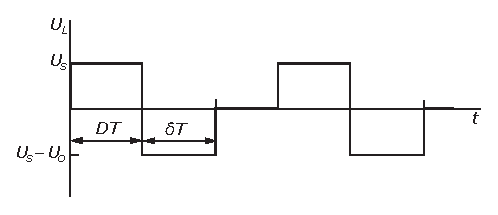
\includegraphics[width=10cm]{gfx/tension_inductor_elevador_MCD.eps}} \\
 \subfloat[Corriente de diodo]{\label{fig:corriente_diodo_elevador_MCD}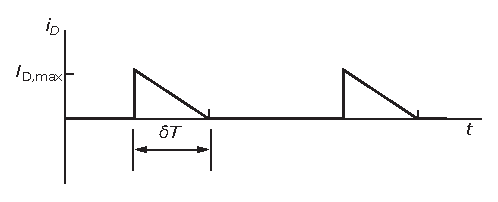
\includegraphics[width=10cm]{gfx/corriente_diodo_elevador_MCD.eps}} \\
 \subfloat[Corriente de inductor]{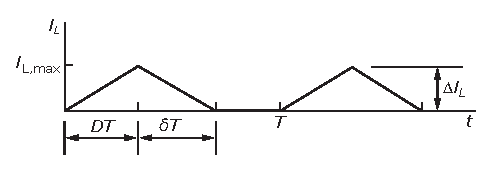
\includegraphics[width=10cm]{gfx/corriente_inductor_elevador_MCD.eps}}
 \caption{Curvas de estado estacionario para el elevador operando en MCC}
 \label{fig:estado_estacionario_elevador_MCD}
\end{figure}

Usando la integral de la tensión en el inductor se obtiene,
$$ U_iD+(U_i-U_o)\delta=0 $$
Siendo $\delta$ el tiempo en sigue habiendo conducción de corriente a través del inductor luego de la apertura del transistor. Esto deriva en las siguientes ecuaciones,

\begin{subequations}
 \begin{equation}
  \frac{U_o}{U_i}=\frac{D+\delta}{\delta}
  \label{eq:relacion_basica}
 \end{equation}
  \begin{equation}
  \frac{I_o}{I_i}=\frac{\delta}{D+\delta}
 \end{equation}
\end{subequations}

Ha aparecido un nuevo parámetro temporal $\delta$ que puede eliminarse usando otras expresiones. Utilizando la fig. \ref{fig:corriente_diodo_elevador_MCD}
se obtiene la corriente continua de salida en términos de los parámetros $D$ y $\delta$:

 $$I_{o}=\frac{U_i D T_s}{2L}\delta=\frac{U_o}{R}$$
 
Se puede despejar $\delta$:

\begin{equation}
 \delta = \frac{U_o}{U_i}\frac{2L}{RDT}
 \label{eq:delta_elevador}
\end{equation}

Sustituyendo la eq. (\ref{eq:delta_elevador}) en la eq. (\ref{eq:relacion_basica}) y resolviendo la ecuación
cuadrática resultante para $\frac{U_o}{U_i}$ se obtiene:

\begin{equation}
 \frac{U_o}{U_i}=\frac{1}{2} \left(1+\sqrt{1+\frac{2D^2RT_s}{L}} \right)
 \label{eq:relacion_elevador_MCD}
\end{equation}

Es posible que el convertidor cambie de modo de operación para una carga fija al variar $D$ ya sea cambiando la referencia de tensión
de salida o debido a variaciones en la tensión de entrada. Esto define intervalos en
la relación de transformación, que dependen del modo de conducción en que opere el equipo. En la 
fig. \ref{fig:caracteristica_elevador_MCD} se muestra un ejemplo de ello.

\begin{figure}[H]
 \centering
 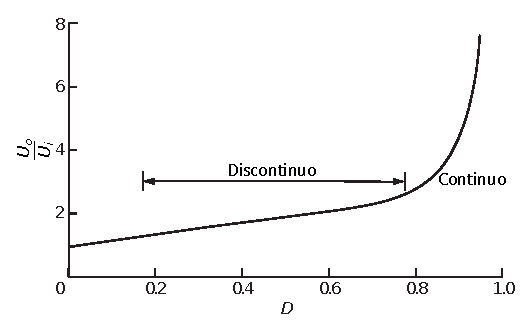
\includegraphics[width=12cm]{gfx/caracteristica_elevador_MCD.eps}
 \caption{Intervalos de modos de conducción para la relación de conversión del elevador.}
 \label{fig:caracteristica_elevador_MCD}
\end{figure}

\subsection{Modelo dinámico}
Las señales de comando del convertidor se obtienen del \emph{hardware} de control que realiza los cálculos necesarios a partir
de los algoritmos con que trabaje. Su estudio y diseño serán abordados en el cap. \ref{ch:control}. Para realizar el diseño, sin
embargo se debe contar con un modelo dinámico. Es por ello que se obtuvo el modelo en variables de estado del sistema considerando 
las pérdidas debidas a los elementos resistivos en serie. El modelo se presenta a continuación,
\[
  \pmb{x}=
  \left(\begin{array}{c}
  i_{L}\\
  u_{C}
  \end{array}\right)
\]

\begin{equation}
\begin{cases}
\pmb{\dot{x}}=\left(\begin{array}{cc}
\frac{-r_{s}}{L} & 0\\
0 & \frac{-1}{RC(1+\frac{r_{C}}{R})}
\end{array}\right)\pmb{x}+\left(\begin{array}{c}
\frac{1}{L}\\
0
\end{array}\right)u_{i}, & 0<t<DT\\
\pmb{\dot{x}}=\left(\begin{array}{cc}
\frac{-(r_{s}(r_{c}+R)+r_{c}R)}{(r_{c}+R)L} & \frac{-1}{(1+\frac{r_{C}}{R})L}\\
\frac{1}{(1+\frac{r_{C}}{R})C} & \frac{-1}{RC(1+\frac{r_{C}}{R})}
\end{array}\right)\pmb{x}+\left(\begin{array}{c}
\frac{1}{L}\\
0
\end{array}\right)u_{i} & DT<t<T
\end{cases}
\end{equation}

\begin{equation}
\begin{cases}
\left(\begin{array}{c}
i_{L}\\
u_{o}
\end{array}\right)=\pmb{y}=\left(\begin{array}{cc}
1 & 0\\
0 & \frac{R}{R+r_{C}}
\end{array}\right)\pmb{x} & 0<t<DT\\
\left(\begin{array}{c}
i_{L}\\
u_{o}
\end{array}\right)=\pmb{y}=\left(\begin{array}{cc}
1 & 0\\
\frac{Rr_{C}}{R+r_{C}} & \frac{R}{R+r_{C}}
\end{array}\right)\pmb{x} & DT<t<T
\end{cases}
\end{equation}

\section{Convertidor reductor}
Este dispositivo sirve para reducir los niveles de tensión de la fuente con la que se lo alimenta. Para el trabajo realizado se dispuso de otro convertidor
elevador idéntico al que se armó para la etapa de adaptación del módulo de pilas de celdas de combustible. Gracias a su diseño fue posible adaptarlo, mediante
ajustes simples, a una topología reductora. El esquemático del circuito reductor se muestra en la fig. \ref{fig:reductor} donde se ha resaltado la
adición de los nuevos componentes sobre el esquemático mostrado en la fig. \ref{fig:elevador}.

Los rangos en los que operará el reductor deben ser adaptables a los del elevador. Esto no supone un problema considerando que uno de los equipos
está  basado en el otro, aunque más adelante se detallan las exigencias a las que será sometido el reductor para asegurar que se mantienen en los rangos
de trabajo permitidos por las hojas de datos de los componentes.

Desde el punto de vista estructural, el convertidor reductor es más sencillo que el elevador ya que la topología se mantiene igual durante cada ciclo de
conmutación. Por lo tanto, la operación de esta configuración puede interpretarse como la aplicación de un filtro pasa-bajos a una señal PWM de amplitud igual 
a la tensión de entrada. De este modo, la tensión devuelta correspondería aproximadamente al valor medio de la señal PWM.

\begin{figure}[H]
 \centering
 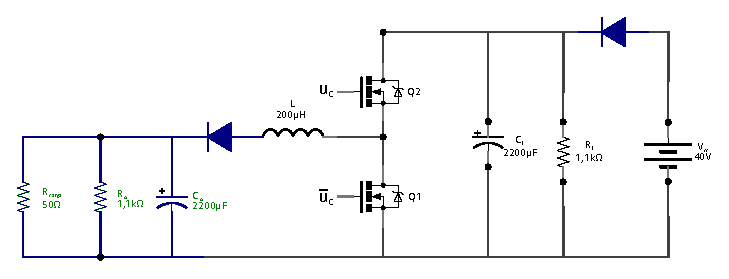
\includegraphics[width=12cm]{gfx/reductor.eps}
 \caption{Esquemático del reductor a partir del circuito del elevador}
 \label{fig:reductor}
\end{figure}

\subsection{Operación en estado estacionario}
Se aplicarán los mismos conceptos vistos en el sec. \ref{sub:elevador_estacionario} para hallar las relaciones que determinan la operación del convertidor
reductor.

\subsubsection{Modo de conducción continua}
Al igual que en el caso del elevador se ha realizado un análisis en estado estacionario del convertidor reductor de cuyos resultados se extrae
suficiente información para decidir sobre la elección de los componentes que serán parte del presente convertidor y para obtener los modelos
a utilizar para el diseño de los algoritmos de control.

En la fig. \ref{fig:reductor_CC} se muestran las curvas para el funcionamiento del convertidor en estado estacionario, para éste caso no es necesario el uso
de las curvas de corriente del diodo.

\begin{figure}
 \centering
 \subfloat[Tensión de inductor]{\label{fig:tension_inductor_reductor_MCC}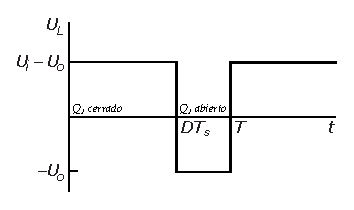
\includegraphics[width=5cm]{gfx/tension_inductor_reductor_MCC.eps}} \quad
 %\subfloat[Corriente de diodo]{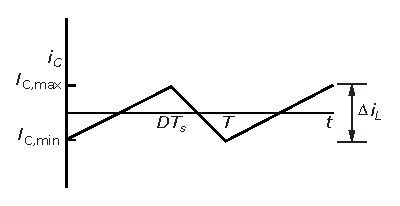
\includegraphics[width=5cm]{gfx/corriente_capacitor_reductor_MCC_simple.eps}} \\
 \subfloat[Corriente de inductor]{\label{fig:corriente_inductor_reductor_MCC}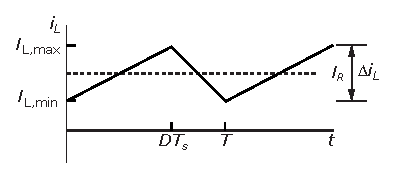
\includegraphics[width=5cm]{gfx/corriente_inductor_reductor_MCC.eps}} \\ \quad
 \subfloat[Corriente de capacitor]{\label{fig:corriente_capacitor_reductor_MCC}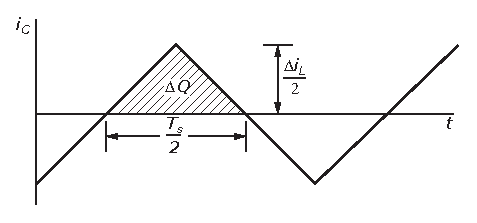
\includegraphics[width=5cm]{gfx/corriente_capacitor_reductor_MCC.eps}}
 \caption{Curvas de estado estacionario para el elevador operando en MCC}
 \label{fig:reductor_CC}
\end{figure}

Mediante los mismos razonamientos utilizados al analizar el elevador se obtienen las relaciones de conversión y los valores límites para la corriente.
A partir de la integral de la tensión del inductor,
$$ (U_i - U_o)D - U_o(1-D)=0 $$
Operando resulta,
\begin{equation}
 \frac{U_o}{U_i}=D
 \label{eq:relacion_reductor}
\end{equation}
Y una vez más, con $P_i=P_o$,
\begin{equation}
 \frac{I_o}{I_i}=\frac{1}{D}
 \label{eq:relacion_corriente_reductor}
\end{equation}

Para analizar el comportamiento de la corriente se asume que la corriente es una onda triangular se usa la (\ref{eq:aprox_corriente})
y se establece que la variación de corriente es igual tanto para el estado cerrado de la llave como el abierto,
\begin{subequations}
  \begin{equation}
   \Delta i_{L,cerrada}=\frac{U_i-U_o}{L}DT_s
  \end{equation}
  \begin{equation}
   \Delta i_{L,abierta}=-\frac{U_o}{L}(1-D)T_s
  \end{equation}
\end{subequations}
Para obtener mayor precisión en los resultados anteriores se consideran los elementos parásitos,
\begin{equation}
 \frac{U_o}{U_i}=\frac{D}{1+\frac{r}{R}}
 \label{eq:relacion_reductor_completa}
\end{equation}
\begin{equation}
 \eta=\frac{P_o}{P_i}=\frac{1}{1+\frac{r}{R}}
 \label{eq:eficiencia_reductor}
\end{equation}
Las ecuaciones \ref{eq:relacion_reductor_completa} y \ref{eq:eficiencia_reductor} reflejan que la relación de conversión
y la eficiencia solo varían por un factor respecto de la relación ideal (en cuyo caso $\eta=1$), además la eficiencia es independiente del ciclo de trabajo,
Esto es favorable ya que no hay necesidad de acotar el rango de trabajo debido a los efectos de los elementos parásitos.

Según la fig. \ref{fig:reductor_CC}, a partir del la variación de corriente por el inductor puede encontrarse el límite entre los dos modos de operación MCC y MCD.

 \begin{equation}
  \bar{i}_{L,min}=\frac{\Delta i_L }{2}= \frac{D T_s(1-D)}{2L}U_i=\frac{T_s(1-D)}{2L}U_o=\bar{i}_{o,min}
  \label{eq:limite_corriente_reductor}
 \end{equation}

Para estudiar las fluctuaciones en la tensión entregada por el convertidor se suman las contribuciones de los efectos de la naturaleza finita de la capacidad
y la ESR. Por lo tanto, a partir de la fig. \ref{fig:corriente_capacitor_reductor_MCC} puede obtenerse la variación en la carga y a partir de esto la variación
en la tensión de salida como se hizo para el caso del elevador.

La variación de carga se obtiene al aplicar reglas geométricas a la fig. \ref{fig:corriente_capacitor_reductor_MCC}:
$$ \Delta Q=\frac{1}{2}\frac{T_s}{2}\frac{\Delta i_L}{2}=\frac{T_s \Delta i_L}{8} $$
Sustituyendo en la expresión anterior:
\begin{equation}
 \Delta U_{o,C}=\frac{T_s \Delta i_L}{8C}=\frac{U_o T_s (1-D)}{8LC}
\end{equation}
\begin{equation}
 \frac{\Delta U_{o,C}}{U_o}=\frac{T_s (1-D)}{8LC}
\end{equation}
En cuanto al efecto de la resistencia parásita se aplica la ley de omh como se hizo en el caso anterior.

\subsubsection{Exigencias eléctricas en estado estacionario para MCC}

Se ha realizado un análisis en estado estacionario del Convertidor Reductor de cuyo análisis se extraerá
suficiente información para decidir sobre la elección de los componentes que serán parte del presente convertidor.
\begin{table}[H]
  \centering
  \begin{tabular}{|c|c|c|c|c|}
  \hline 
  Comp. & $T_{1}$ & $T_{2}$ & $L$ & $C$\tabularnewline
  \hline 
  \hline 
  $U_{max}$ & $U_{o}$ & $U_{o}$ & $U_{o}-U_{i}$ o $U_{o}$ & $U_{o}$\tabularnewline
  \hline 
  $U_{ef}$& $U_{o}\sqrt{1-D}$ & $U_{o}\sqrt{D}$ & $\sqrt{(U_{i}-U_{o})^{2}D+U_{o}^{2}(1-D)}$ & $U_{o}$\tabularnewline
  \hline 
  $I_{max}$ & $I_{o}+\frac{U_{o}(1-D)}{2Lf}$ & $I_{o}+\frac{U_{o}(1-D)}{2Lf}$ & $I_{o}+\frac{U_{o}(1-D)}{2Lf}$ & $\frac{U_{o}(1-D)}{2Lf}$\tabularnewline
  \hline 
  $I_{ef}$ &  &  & $\sqrt{I_{o}^{2}+\frac{1}{3}\left(\frac{U_{o}(1-D)}{Lf}\right)^{2}}$ & $\frac{U_{o}(1-D)}{\sqrt{3}Lf}$\tabularnewline
  \hline 
  \end{tabular}
  \caption{Exigencias eléctricas de los componentes del reductor.}
  \label{tab:exigencias_reductor}
\end{table}
\subsubsection{Modo de conducción discontinua}
Cuando la corriente disminuye por debajo del margen de la eq. (\ref{eq:limite_corriente_reductor} el dispositivo entra conducción discontinua y cuando eso ocurre, las
características cambian al igual que ocurre para el elevador. Con ayuda de las figs. \ref{fig:estado_estacionario_reductor_MCD} se obtienen los desarrollos presentados 
a continuación.

\begin{figure}
 \centering
 \subfloat[Tensión de inductor]{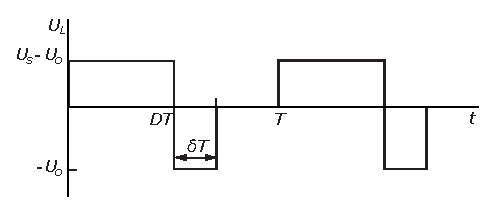
\includegraphics[width=10cm]{gfx/tension_inductor_reductor_MCD.eps}} \\
 \subfloat[Corriente de diodo]{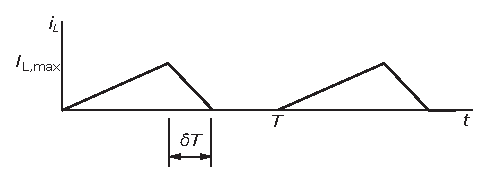
\includegraphics[width=10cm]{gfx/corriente_inductor_reductor_MCD.eps}} \\
 \subfloat[Corriente de inductor]{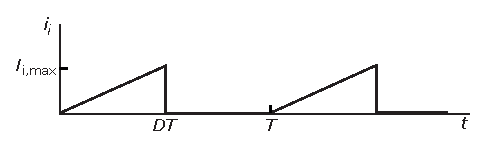
\includegraphics[width=10cm]{gfx/corriente_fuente_reductor_MCD.eps}}
 \caption{Curvas de estado estacionario para el elevador operando en MCC}
 \label{fig:estado_estacionario_reductor_MCD}
\end{figure}
Estudiando nuevamente la integral de la tensión en el inductor,
$$ (U_i-U_o)D-U_o\delta=0 $$
Reordenando se tiene,
\begin{equation}
 \frac{U_o}{U_i}=\frac{D}{D+\delta}
 \label{eq:relacion_reductor_MCD}
\end{equation}
Por otra parte, para la corriente,
\begin{equation}
 \Delta i_{L}=\frac{U_i-U_o}{L}DT_s=\frac{U_o\delta T_s}{L}
\end{equation}
Asumiendo constante la tensión de salida,
\begin{equation}
 I_o=\frac{U_o}{R}=\frac{1}{2}\Delta i_L(D+\delta)=\frac{1}{2}\frac{U_i-U_o}{L}DT_s(D+\delta)
\end{equation}
Usando (\ref{eq:relacion_reductor_MCD}) y reordenando se llega a una ecuación de segundo grado, de cuyas soluciones, se usa la que produce valores positivos,
\begin{equation}
 \delta=\frac{-D+\sqrt{D^2+\frac{8L}{RT}}}{2}
\end{equation}
Sustituyendo en la eq. (\ref{eq:relacion_reductor_MCD}),
\begin{equation}
 \frac{U_o}{U_i}=\frac{2D}{D+\sqrt{D^2+\frac{8L}{RT}}}
\end{equation}
Si se fija la corriente de carga puede provocar que la característica del reductor adopte un comportamiento
mixto respecto a los modos de conducción operando en gran parte del rango del ciclo de trabajo
($D$), esto quiere decir que para estos casos el convertidor puede conmutar entre MCC y MCD. Esto se ilustra en la 
fig. \ref{fig:caracteristica_reductor_MCD}.
\begin{figure}
 \centering
 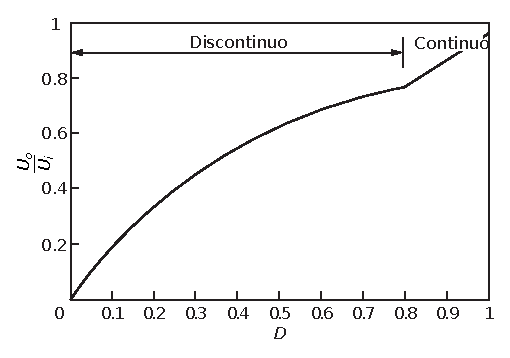
\includegraphics[width=12cm]{gfx/caracteristica_reductor_MCD.eps}
 \caption{Intervalos de modos de conducción para la relación de conversión del reductor.}
 \label{fig:caracteristica_reductor_MCD}
\end{figure}
\subsection{Modelo dinámico}
En esta instancia se presenta el modelo del sistema dinámico del reductor.

\begin{equation}
  \pmb{x}=
  \left(\begin{array}{c}
  i_{L}\\
  u_{C}
  \end{array}\right)
\end{equation}
  
\begin{equation}
  \begin{cases}
  \pmb{\dot{x}}=\left(\begin{array}{cc}
		      \frac{-(r_{s}(r_{c}+R)+r_{c}R)}{(r_{c}+R)L} 	& \frac{-1}{(1+\frac{r_{C}}{R})L}\\
		      \frac{1}{(1+\frac{r_{C}}{R})C} 				& \frac{-1}{RC(1+\frac{r_{C}}{R})}
  \end{array}\right)\pmb{x}+\left(\begin{array}{c}
				  \frac{1}{L}\\
				  0
  \end{array}\right) & 0<t<DT\\
  \pmb{\dot{x}}=\left(\begin{array}{cc}
			\frac{-(r_{s}(r_{c}+R)+r_{c}R)}{(r_{c}+R)L} 	& \frac{-1}{(1+\frac{r_{C}}{R})L}\\
			\frac{1}{(1+\frac{r_{C}}{R})C} 				& \frac{-1}{RC(1+\frac{r_{C}}{R})}
  \end{array}\right)\pmb{x}+\left(\begin{array}{c}
				  0\\
				  0
  \end{array}\right) & DT<t<T
  \end{cases}
\end{equation}


\begin{equation}
  \begin{cases}
  \left(\begin{array}{c}
  i_{L}\\
  u_{o}
  \end{array}\right)=\pmb{y}=\left(\begin{array}{cc}
  1 & 0\\
  \frac{Rr_{C}}{R+r_{C}} & \frac{R}{R+r_{C}}
  \end{array}\right)\pmb{x} & DT<t<T\\
  \left(\begin{array}{c}
  i_{L}\\
  u_{o}
  \end{array}\right)=\pmb{y}=\left(\begin{array}{cc}
  1 & 0\\
  \frac{Rr_{C}}{R+r_{C}} & \frac{R}{R+r_{C}}
  \end{array}\right)\pmb{x} & DT<t<T
  \end{cases}
\end{equation}

Este sistema esta siempre definido por la misma matriz de estados simplificando su análisis, en efecto, el cambio se produce solo sobre
excitación. Por lo tanto puede pensarse que la salida es una señal de pulsos de ancho modulado cuya amplitud corresponde a la tensión de entrada. 

\section{Detalles técnicos de los convertidores utilizados}
Si bien se desarrolló de forma genérica la teoría general de convertidores, en esta sección se presentarán las especificaciones bajo las cuales funcionan
los equipos armados usando la teoría expuesta.

\begin{table}[H]
  \centering
  \begin{tabular}{|c|>{\centering}p{2.5cm}|c|c|c|c|c|}
  \hline 
  Componente & $R_{s}$ & $L$ & $C$ & $I_{ef}$ & $\hat{I}$ & $\hat{U}$\tabularnewline
  \hline 
  \hline 
  Inductor   & $21m\Omega$ $(DC)$ $33m\Omega$ $(AC)$ & $200\mu H$ & - & $15A$ & $16,7A$ & -\tabularnewline
  \hline 
  Capacitor & $50m\Omega$ &  - & $2,2mF$ & $8A$ & - & $100V$\tabularnewline
  \hline 
  Transistor(IRFP-250) & $85m\Omega$ $(r_{T})$ $200m\Omega$ $(r_{D})$ & - & - & $30A$ & $120A$ & $200V$\tabularnewline
  \hline 
  \end{tabular}
  \caption{Especificaciones de los componentes utilizados}
  \label{tab:especificaciones}
\end{table}

\subsection{Convertidor elevador}
El \emph{hardware} correspondiente al elevador construido ha sido diseñado para actuar bajo las siguientes condiciones de operación:

\begin{table}[H]
  \centering
  \begin{tabular}{|c|c|}
  \hline 
  Magnitud & \tabularnewline
  \hline 
  \hline 
  Potencia neta nominal & 300W\tabularnewline
  \hline 
  Tensión de salida nominal & 60V\tabularnewline
  \hline 
  Corriente de salida nominal & 5A\tabularnewline
  \hline 
  Tensión máxima de entrada & 50V\tabularnewline
  \hline 
  Tensión máxima de salida & 100V\tabularnewline
  \hline 
  Corriente máxima en la entrada & 18,5A\tabularnewline
  \hline 
  Corriente máxima en la salida & 5,5A\tabularnewline
  \hline 
  Frecuencia de conmutación & 20kHz\tabularnewline
  \hline 
  Variación de corriente ($ \Delta i_L $) & 3,75A\tabularnewline
  \hline
  \end{tabular}
  \caption{Condiciones de operación para el elevador}
  \label{tab:especificaciones_elevador}
\end{table}

Los límites de las magnitudes anteriores sirvieron de referencia para los ajustes realizados sobre el
acondicionamiento de los circuitos de medida. Estos valores corresponden a los valores máximos según el
circuito acondicionamiento de señales, teniendo en cuenta los rangos
de los sensores involucrados.

Por otro lado es necesario considerar las exigencias que tendrán los componentes operando bajo las condiciones anteriores. Esto se verifica usando el
análisis del circuito en condiciones de estado estacionario. Usando la información listada en el cuadro \ref{tab:especificaciones_elevador} 
junto con las expresiones en el cuadro \ref{tab:exigencias_elevador} se obtienen
las solicitaciones eléctricas a las que serán sometidos los componentes del convertidor elevador que se muestran en el cuadro \ref{tab:solicitaciones_elevador}.

\begin{table}[H]
  \centering
 \begin{tabular}{|c|c|c|c|c|}
  \hline 
  Componente & $T_{1}$ & $T_{2}$ & $L$ & $C$\tabularnewline
  \hline 
  \hline 
  Tensión pico & $60V$ & $60V$ & $<60V$ & $60V$\tabularnewline
  \hline 
  Tensión eficaz & $43V$ & $43V$ & $30V$ & $60V$\tabularnewline
  \hline 
  Corriente pico & $8A$ & $8A$ & $8A$ & $6A$\tabularnewline
  \hline 
  Corriente eficaz &  &  & $9A$ & $4A$\tabularnewline
  \hline 
 \end{tabular}
 \caption{Requerimientos a los componentes del elevador}
 \label{tab:solicitaciones_elevador}
\end{table}

Se han realizado simulaciones para validar el estudio utilizando los valores reales de los componentes con los que se armaron las placas.
En la fig. \ref{fig:boostCC} se presentan las curvas de operación en estado estacionario para el convertidor elevador operando a $D=75\%$ y una corriente de
aproximadamente $6A$.
También se han ejecutado simulaciones para las condiciones de trabajo en MCD que se muestran en la fig. \ref{fig:boostCD} en las que se ha fijado
un ciclo de trabajo de $D=25\%$ y una corriente de carga de $1.8A$.
\begin{figure}
 \centering
 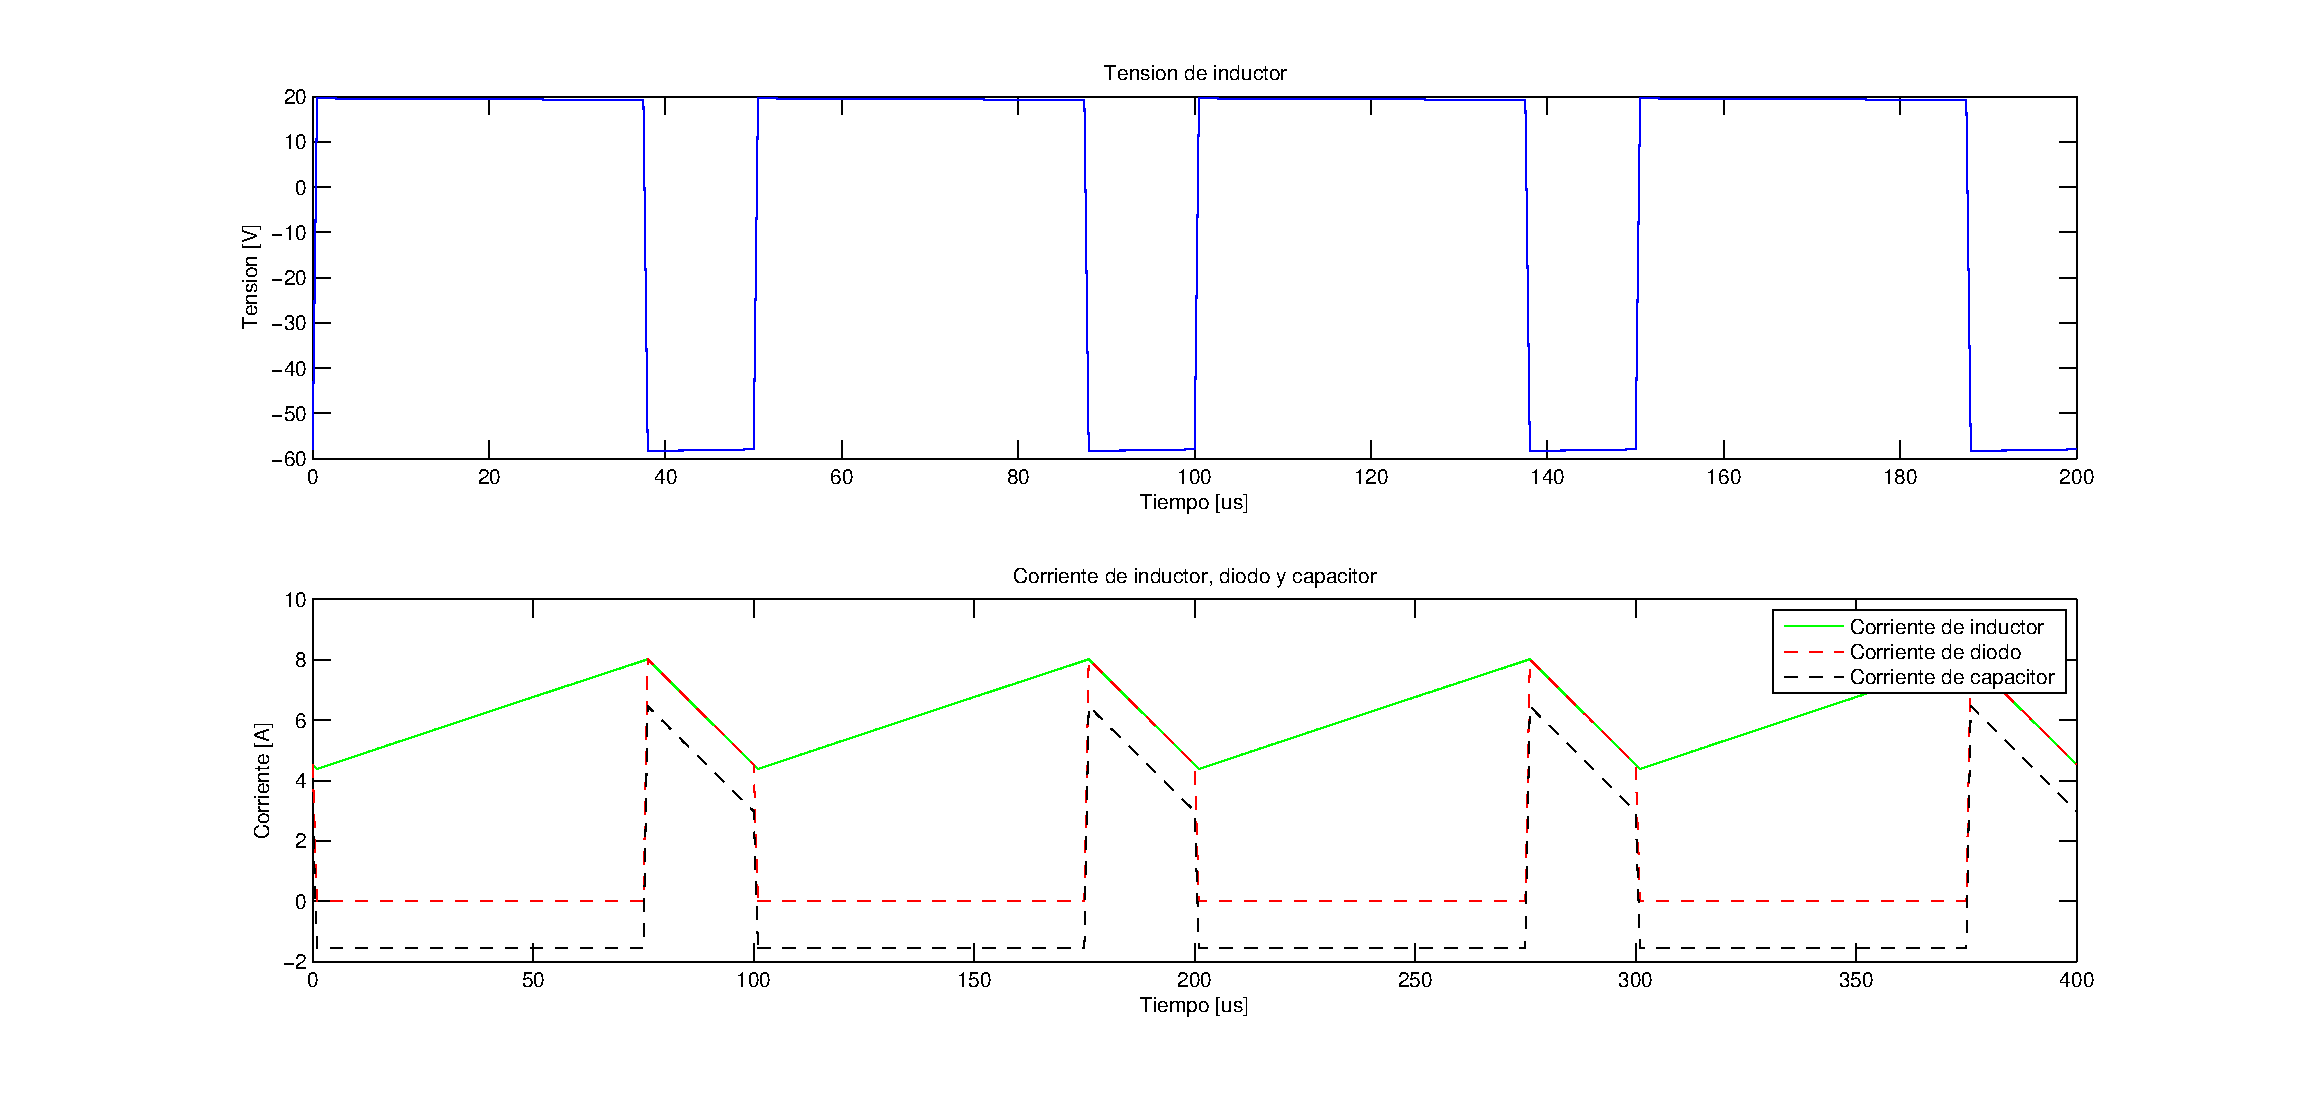
\includegraphics[width=12cm]{gfx/boostCC.eps}
 \caption{Convertidor elevador operando en MCC}
 \label{fig:boostCC}
\end{figure}

\begin{figure}
 \centering
 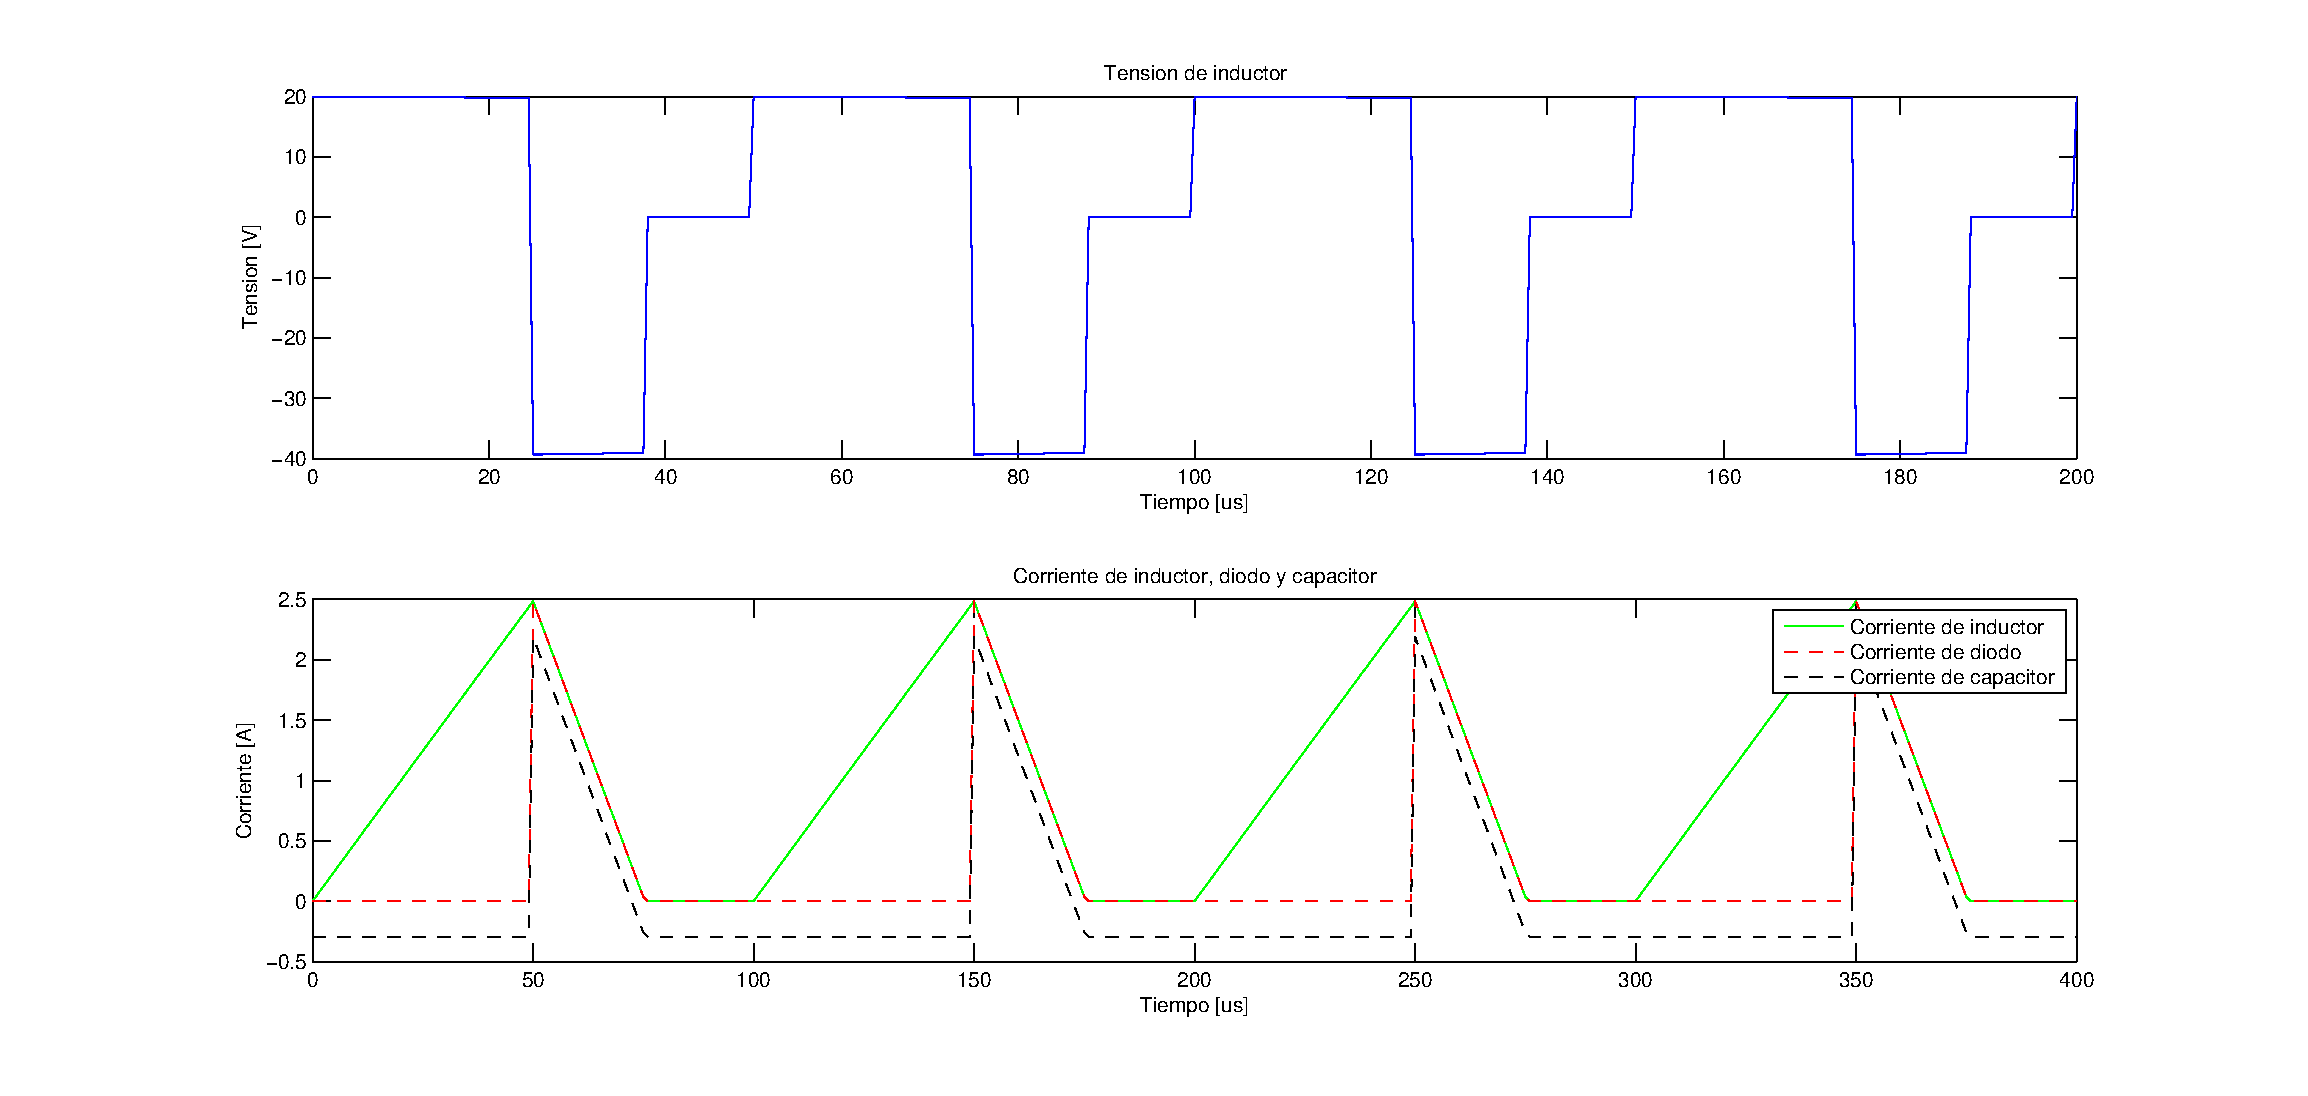
\includegraphics[width=12cm]{gfx/boostCD.eps}
 \caption{Convertidor elevador operando en MCD}
 \label{fig:boostCD}
\end{figure}

\subsection{Convertidor reductor}
A partir del esquemático y las magnitudes de trabajo del elevador se pueden inferir las condiciones de operación para el reductor, que
se listan en el siguiente cuadro:

\begin{table}[H]
  \centering
  \begin{tabular}{|c|c|}
  \hline 
  Magnitud & \tabularnewline
  \hline 
  \hline 
  Potencia neta nominal & 300W\tabularnewline
  \hline 
  Tensión de salida nominal & 30V\tabularnewline
  \hline 
  Corriente de salida nominal & 10A\tabularnewline
  \hline 
  Tensión máxima de entrada & 50V\tabularnewline
  \hline 
  Tensión máxima de salida & 50V\tabularnewline
  \hline 
  Corriente máxima en la entrada & 10A\tabularnewline
  \hline 
  Corriente máxima en la salida & 15A\tabularnewline
  \hline 
  Frecuencia de conmutación & 20kHz\tabularnewline
  \hline 
  Variación de corriente ($ \Delta i_L $) & 3A\tabularnewline
  \hline
  \end{tabular}
  \caption{Condiciones de operación para el elevador}
  \label{tab:especificaciones_reductor}
\end{table}

Al igual que para el convertidor elevador se pueden obtener las exigencias eléctricas a las que se someten los componentes del reductor, según
el análisis de estado estacionario del mismo. Estos datos se han calculado considerando la utilización de los mismos componentes que los del
elevador. La tabla \ref{tab:solicitaciones_reductor} muestra esto.

\begin{table}[H]
  \centering
  \begin{tabular}{|c|c|c|c|c|}
  \hline 
  Componente & $T_{1}$ & $T_{2}$ & $L$ & $C$\tabularnewline
  \hline 
  \hline 
  Tensión pico & $40V$ & $40V$ & $<40V$ & $40V$\tabularnewline
  \hline 
  Tensión eficaz & $28V$ & $28V$ & $20V$ & $40V$\tabularnewline
  \hline 
  Corriente pico & $15A$ & $15A$ & $15A$ & $1,2A$\tabularnewline
  \hline 
  Corriente eficaz &  &  & $15A$ & $1,4A$\tabularnewline
  \hline 
  \end{tabular}
  \caption{Requerimientos a los componentes del reductor}
  \label{tab:solicitaciones_reductor}
 \end{table}
 
A fin de obtener una referencia del funcionamiento cuantitativo del convertidor se han ejecutado algunas simulaciones
con ciclos de trabajo y cargas fijas, tal como se realizó para el elevador. Para el caso de la operación en modo de 
conducción continua las curvas obtenidas se muestran en la fig. \ref{fig:buckCC} que opera con un ciclo de trabajo de
$D=75\%$ y entregando aproximadamente $1A$. En contraste, la fig. \ref{fig:buckCD} muestra las curvas del convertidor
trabajando en MCD con un ciclo de trabajo de $D=25\%$ y una carga aproximada de $600mA$.
 
\begin{figure}[H]
 \centering
 \includegraphics[width=12cm]{gfx/buckCC.eps}
 \caption{Convertidor reductor operando en MCC}
 \label{fig:buckCC}
\end{figure}

\begin{figure}[H]
 \centering
 \includegraphics[width=12cm]{gfx/buckCD.eps}
 \caption{Convertidor reductor operando en MCD}
 \label{fig:buckCD}
\end{figure}

\section{Comentarios}
A lo largo del capítulo se han introducido los conceptos elementales que definen los rasgos fundamentales de los convertidores conmutados y
se ha mostrado cómo se manifiestan el comportamiento de los convertidores mediante la variación de los parámetros que los definen. Esta
información será de vital importancia para el desarrollo que sigue, orientado al control de estos dispositivos. 

Los convertidores de potencia DC-DC se controlan a través del estado de sus llaves. Su comportamiento y desempeño esta
fuertemente asociado a los parámetros temporales que surgen del modo en que se operan estas llaves, y estos resultados se utilizaron para el 
planteo de los algoritmos explicados en el capitulo siguiente.

Además, se presentaron las características prácticas generales que detallan los componentes empleados en el armado de las placas y del mismo
modo, los cambios realizados para la obtención de la plataforma utilizada para el emulador.
\end{comment}

\chapter{Modelización}
\label{ch:modelizacion}
\lhead{\emph{Modelización}}

\todo[inline]{Aca viene todo sobre el modelo de la antena programado}

\section{Modelización de los acoplamientos mútuos}

Los acoplamientos mútuos fueron modelados como si fuese un cable

\section{Modelo de la antena}

El modelo de antena está programado de tal forma que se lo pueda utilizar para simular una antena con parámetros de RF,
la misma está conformada por los siguientes componentes: cables, psc, trms, defasadores y elementos radiantes. Como es 
requerido calibrar con dos métodos de calibración una misma antena en un estado determinado, para poder comparar los resultados
obtenidos, se opta por guardar en archivos tanto la configuración como el comportamiento de la misma. 

La modelizaci\'on de los componentes en RF es utilizando los par\'ametros S 
En el apéndice 
\ref{AppendixC} se muestra un ejemplo de estos archivos para una antena de dos módulos radiantes.

El simulador es de dos etapas, la primera parte es la encargada de la modelización de la antena y sus componentes, y la 
segunda, de calibrar dicho modelo. La figura \ref{fig:prog_inic} muestra de forma simplificada el flujo de ejecuci\'on del 
programa.

\begin{figure}
 \centering
 \includegraphics[width=10cm]{gfx/FlujoEjecucion.png}
 \caption{Flujo de ejecuci\'on del modelo de antena.}
 \label{fig:prog_inic}
\end{figure}

\subsection{Generador de Antena}

En principio, una antena necesita que todos los caminos entre el punto donde se inyecta o recibe la se\~nal y los m\'odulos 
radiantes sean iguales. Esta caracter\'istica es similar a la de un \'arbol balanceado. Por lo tanto, para definir la 
estructura interna de la antena, se definen simplmenete los elementos que conforman dicho \'arbol y, para determinar el orden 
de armado de la antena, se utiliza una lista. El orden es descendiente, si se para en un elemento de la lista, los de la 
izquierda son ascendientes y los de la derecha son descendientes. En la figura \ref{fig:2RMAntenna} se muestra la antena que 
se construye teniendo como configuración: [\enquote*{cable1}, \enquote*{psc12}, \enquote*{cable2}, \enquote*{trm}, 
\enquote*{circulator}, \enquote*{cable3}, \enquote*{rm}].

Es necesario definir cuales son las características físicas de cada uno de los componentes mencionados en la lista anterior. 
La tabla \ref{tab:propertiesOfComponents} determina las propiedades de cada elemento contenido dentro de una antena. 

\begin{table}[H]
  \footnotesize
  \centering
  \begin{tabular}{|c|c|}
	\hline
	\textbf{Componente de Antena} & \textbf{Cacarcterísticas físicas} \tabularnewline \hline 
	\multirow{2}{*}{cable} &  attenuation [db] \tabularnewline \cline{2-2}
	 & length [m] \tabularnewline \hline 
	\multirow{2}{*}{TRM} & gain [db]\tabularnewline \cline{2-2}
	 & phaseShift [deg] \tabularnewline \hline 
	PSC1$j$ & outputPorts = $j$ \tabularnewline \hline 
	circulator & \tabularnewline \hline 
	RM & \tabularnewline \hline 
  \end{tabular}
  \caption{Propiedades físicas de cada componente de una antena}
  \label{tab:propertiesOfComponents}
\end{table}

\begin{figure}
 \centering
 \includegraphics[width=10cm]{gfx/RFDN.png}
 \caption{Estructura interna de una de las polarizaciones de una antena con dos elementos radiantes.}
 \label{fig:2RMAntenna}
\end{figure}

Con estos componentes, si bien está definida la cantidad de elementos radiantes, falta definir las dimensiones de la antena, 
en otras palabras, la cantidad de paneles, la cantidad de elementos por panel y la separación, tanto horizontal como vertical,
entre elementos. Los primeros se traducen a cantidad de columnas y filas de RMs. 

Como dicha información es medianamente redundante y posiblemente incompatible con la definición de la estructura interna de 
la antena, es necesario un chequeo de compatibilidad. La figura \ref{fig:frontAntenna} muestra el frente de una antena que se 
construye teniendo como configuración: "quantityRows": 1, "quantityColumns": 2, "verticalSeparation": 0.2, 
"horizontalSeparation": 0.2.

\begin{figure}
 \centering
 \includegraphics[width=5cm]{gfx/FrontAntenna2.png}
 \caption{Frente de antena de dos elementos radiantes.}
 \label{fig:frontAntenna}
\end{figure}

Una vez obtenida la estructura de la antena, es necesario determinar que componentes van a tener desvíos en el comportamiento 
deseado. Para ello, se agrega una lista indicando que componentes se desea que tengan errores. Los errores tienen una 
distribución gaussiana con media 0. El desvío estandar es configurable.
\todo[inline]{pablo, saco o dejo esta parte??}

Para el caso en que se desee realizar la calibración en el modo Completo, se debería agregar errores de planitud de la antena.
Para ello, los errores se verían reflejados en el archivo de la configuración del panel de la antena. De todas formas, a modo 
como el modelo se realizó para validar el método, solamente se realizó el modelo de la planitud ideal.


\todo{Poner un gráfico donde se defina una antena de 2 elementos radiantes}

\todo{hacer grafico de clases del generador de antena}

\subsection{Calibrador}

A la hora de calibrar, la primer configuración es la del apuntamiento deseado. Para ello, se tienen que configurar la fase de 
los defasadores de cada elemento radiante de la polarización a transmitir.
elementos radiantes de la polarización a transmitir   


\todo{hacer grafico de clases del calibrador de antena}



Al tener cada componente de la antena caracterizado como se va a comportar, se puede determinar la matriz de parámetros de la
totalidad de la antena, tanto para transmisión como recepción en la polarización deseada.

\todo{agregar el grafico de la composicion de una antena}

Como una misma antena se la podía llegar a calibrar con los dos métodos, se optó por utilizar archivos json. En los cuales 
se guarda la configuración y propiedades físicas tanto del panel como de la RFDN. Las propiedades del primer grupo es 
simplemente la distancia de todos a todos los elementos y las del segundo grupo, corresponden a la matriz de parámetros S y 
que componente tienen conectado en los conectores de salida. En el anexo \ref{AppendixC} se puede observar un ejemplo de estos archivos
para una antena con dos elementos radiantes.

\subsection{Configuraciones del sistema}

Las configuraciones que se le pueden realizar al modelo de antena para realizar los distintos ensayos están listados en la 
tabla \ref{tab:conf_modelo_antena}.

\begin{center}
  \footnotesize
  \centering
  \begin{longtable}{|c|p{9cm}|}
    \hline 
	\multicolumn{2}{|c|}{\textbf{Parámetros de entrada}} \\ 
	\hline
    Frequencia		& Es la frecuenia central de trabajo en Hz \tabularnewline \hline 
    Potencia		& Potencia con la que se alimenta la antena en db \tabularnewline \hline 
    Fase			& Fase con la que se alimenta la antena en grados \tabularnewline \hline 
    Row Steering	& Apuntamiento horizontal que se le quiere dar al beam de salida, en grados  \tabularnewline \hline 
    Column Steering	& Apuntamiento vertical que se le quiere dar al beam de salida, en grados  \tabularnewline \hline 
	\multicolumn{2}{|c|}{\textbf{Parámetros de calibración}} \\ 
	\hline
	potencia Tx deseada	& Potencia de transmisión deseada para calbirar  \tabularnewline \hline 
	potencia Rx deseada	& Potencia de recepción deseada para calbirar  \tabularnewline \hline 
	Errores	& Son los errores referentes a la hora de calibrar el modelo de antena. Pueden ser: interPulseGainChirpError, interPulsePhaseChirpError, gainChirpRepError, phaseChirpRepError, WalPhaseErrors  \tabularnewline \hline
	\multicolumn{2}{|c|}{\textbf{Parámetros de Antena}} \\ 
	\hline
	Cantidad Filas	& Da la cantidad de módulos radiantes en dirección vertical \tabularnewline \hline 
	Cantidad Columnas	& Da la cantidad de módulos radiantes en dirección horizontal \tabularnewline \hline 
	Separación vertical & Es la separación vertical entre RMs \tabularnewline \hline 
	Separación horizontal & Es la separación horizontal entre RMs \tabularnewline \hline 
	Secuencia de componentes & Es la secuencia de componentes que conforma la RFDN, los mismos pueden ser: cables, psc, trm, circulador, rm \tabularnewline \hline 
	Errores  & Son los componentes de la antena que pueden tener errores. Los mismos pueden ser: RMError, TRMError, CirculatorError, PSCError \tabularnewline \hline 
	TRMs muertos & Es una lista que indica que trms están muertos en el panel de la antena. \tabularnewline \hline 
	\multicolumn{2}{|c|}{\textbf{Componentes de Antena}} \\
	\hline
	$cable_i$ & Se pueden definir tantos cables como se deseen, los parámetros a definir son: attenuation [db], length [m], type = cable \tabularnewline \hline 
	$trm_i$ & Se pueden definir tantos TRMs como se deseen, los parámetros a definir son: gain [db], phaseShift [deg], type = TRM \tabularnewline \hline 
	$psc_{1j}$ & Se pueden definir tantos PSC como se deseen, los parámetros a definir son: outputPorts = $j$, type = PSC1$j$ \tabularnewline \hline 
	circulator & aca se puede definir un circulador, el parámetro a definir es: type = circulator \tabularnewline \hline 
	$rm$ & Se puede definir un RM, el parámetro a definir es: type = RM \tabularnewline \hline 
	\multicolumn{2}{|c|}{\textbf{Desvío estandard del error}} \\
	\hline
	Error del cable & Desvío estandard de los cables. \tabularnewline \hline 
	Error del circulador & Desvío estandard de los circuladores. \tabularnewline \hline 
	Error del TRM & Desvío estandard de los TRMs. \tabularnewline \hline 
	Error del PSC & Desvío estandard de los PSC. \tabularnewline \hline 
	Error del RM & Desvío estandard de los RM. \tabularnewline \hline 
	Error de ganancia entre pulsos & Desvío estandard de ganancia entre pulsos de calibración. \tabularnewline \hline 
	Error de fase entre pulsos & Desvío estandard de fase entre pulsos de calibración. \tabularnewline \hline 
	Error de ganancia de la chirp replica & Desvío estandard de ganancia de la chirp replica. \tabularnewline \hline 
	Error de fase de la chirp replica & Desvío estandard de fase de la chirp replica. \tabularnewline \hline 
	Error de fase del walsh & Desvío estandard de fase del seteo de los defasadores en calibración. \tabularnewline \hline 
	\caption{Configuraciones del modelo de antena}
  \end{longtable}
  \label{tab:conf_modelo_antena}
\end{center}

A su vez, también se puede configurar que tipo de calibración se desea para poder obtener los resultados, se pueden graficar 
los patrones de antena deseados en el corte de azimuth/rango deseados 

El acoplamiento mútuo se lo modeliza como si fuese un cable pero con las propiedades de atenuación y defasaje de una onda en
el vacío. Las cuales son:

\todo{Poner que significa el alfa}
\begin{equation}
	c = \dfrac{e^{-2\alpha r}}{4\pi r^2}
\end{equation}





\todo{poner en algun lado que se sugiere para medir la fase de medir en un unico punto lo que defasa la antena punta a punta una unica vez y se lo carga al metodo}
Una antena se calibra buscando que no solo todos los caminos de recepción atenúen y defasen exactamente lo mismo, sino que 
también sea un valor conocido. Para transmisión se busca lo mismo, con la salvedad que se puede modificar la fase de la 
señal que se emite en algunos RMs para modificar el lugar de apuntamiento de la antena.

Hay distintos factores que hacen que los componentes dejen de comportarse de forma nominal, por ejemplo se puede nombrar el
cambio de temperatura, el mero envejecimiento de los componentes al pasar el tiempo, que un mero cable se haya doblado más
de la cuenta, interferencias electromagnéticas, radiadas o conducidas, o entre distintos componentes, etc. 

Es importante que un patrón de antena posea los lóbulos secundarios lo más chicos posibles con respecto al lóbulo principal,
que el lóbulo principal sea lo más angosto posible, con esto se aumenta la resolución espacial. Un factor que ocurre es el 
de los targets ficticios.\todo{no se como se elimina}


\todo{poner que factores hacen que cambie la ganancia de los componentes para calibrar la antena}
\todo{poner que ocurre con el antnena pattern si no está correctamente calibrada, altura de lóbulos secundarios, ancho 
de lóbulo principal, pico del lóbulo principal, etc}

Para poder calibrar esta antena polarimétrica haciendo uso de los acoplamientos mutuos, se cuenta con el uso de 
cuadrados mínimos. La idea es realizar lazos de calibración transmitiendo en una polarización y recibiendo en la
otra a la vez. Para esto, es necesario que no solo se pueda configurar algunos RMs em modo $T_x$ y otros en modo $R_x$ en 
distintas polarizaciones, sino también poder configurar los módulos que no forman parte de dicho lazo en modo alta 
impedancia (en este modo el módulo no transmite ni recibe nada, evitando así la inyección de ruido y señal en zonas 
indeseadas de la antena). 

Tomando como caso una antena rectangular de $M x N$ módulos radiantes y asumiendo que solo se transmite y recibe de a un 
RM por lazo de calibración, a priori, se dispone de un máximo de $(MN)^2$ ecuaciones. La cantidad de incógnitas de todos
los caminos de la RFDN, tanto transmisión como recepción en ambas polarizaciones (H y V), son $4MN$. A su vez, en el 
apéndice \ref{AppendixA} se realiza el cálculo de la cantidad de acoplamientos mutuos que posee una antena polarimétrica,
particularmente, la ecuación \ref{eq:amountMutCoupling} muestra la cantidad de incógnitas, que, para este caso, resulta 
ser de $MN(MN-1)/2$. Totalizando en $MN(MN + 7)/2$ incógnitas.

Para que el sistema tenga solución, la cantidad de ecuaciones debe ser mayor que la de incógnitas. Esta restricción solo 
se cumple si se calibra toda la antena en un solo paso (Tx y Rx en ambas polarizaciones) porque es el único caso en que 
cada acoplamiento mútuo aparezca más de una única vez. En caso contrario, habrían siempre más incógnitas que ecuaciones.

\todo{tener en cuenta que por ahora el requerimiento es que la antena sea totalmente plana}

\begin{comment}

Una vez definido el modelo matemático que se pretende emular y el soporte físico sobre el cuál ejecutarlo, se procede a la aplicación del instrumento
que permitirá enlazar las dos partes del proyecto: el control.

Los sistemas de control constituyen una herramienta muy poderosa para la resolución de problemas en ingeniería. Las técnicas que proporciona son de
esencial importancia para el diseño de sistemas complejos. En electrónica, la aplicación de los recursos que proporciona el control automático son
ampliamente utilizados y cada vez encuentran más aplicaciones y de mejor desempeño, gracias al avance de los sistemas embebidos en los últimos tiempos.

Los sistemas digitales modernos han ofrecido un soporte muy robusto a la teoría de control, posibilitando la implementación de funciones y técnicas
que de otro modo serían impracticables. El uso de las herramientas de control mediante sistemas embebidos tiene la gran ventaja, frente a 
mecanismos analógicos, de ser realizados por medio de la programación de los algoritmos que definen la operación a efectuar, de modo que permiten
gran libertad y rigidez al diseño.

Los equipos de potencia electrónicos tienen grandes exigencias temporales para la operación que realizan, tal es el caso de los convertidores conmutados
que requieren de una razonable velocidad de conmutación de las llaves electrónicas que los componen. Es por ello que la electrónica de potencia recibe una
ayuda indispensable del control de sistemas discretos.

El \emph{hardware} utilizado consiste en un DSP que posee varios módulos, de los cuales varios han sido utilizados tanto para hacer cálculos, relevar
mediciones o entregar señales de control. La programación ha sido realizada progresivamente por medio de dos entornos de programación, uno de nivel más
alto y otro de más bajo nivel que contiene el compilador del código que es programado directamente en el dispositivo.

Este capítulo presenta la teoría utilizada para la realización de del trabajo así como los modelos completos de los sistemas implementados. Los elementos
explicados y utilizados van desde filtros digitales hasta controladores elementales y el promediado de sistemas de estructura variable.

\section{Introducción}
Existen diversas opciones al momento de aplicar una estrategia de control a un sistema dado, y además muchas de éstas vienen combinadas entre sí. Para el
abordaje del problema del control de un sistema se establecen ciertos procedimientos que involucran la gestión de la información tomada del sistema (medidas,
modelos, por ejemplo) y el modo en que las acciones de control interactúan con el sistema mencionado. La disposición de estas interacciones es la arquitectura
de control.

La disposición más común en la arquitectura de control, es sin duda la realimentación. Este es un concepto fundamental de la teoría de control y ofrece una multitud
de mejoras al desempeño de los sistemas si ha sido correctamente empleada. Su principio subyace en que a pesar de no conocer con precisión la naturaleza del 
sistema que se controla, se realizan correcciones en las acciones de control utilizando la información medida del efecto que produce el ajuste de sus variables de entrada.

La realimentación puede darse de varias maneras, aunque la aplicación más sencilla consiste en simplemente en obtener la diferencia entre la variable que se 
desea controlar y cierta referencia. A este resultado se le llama error, y dado que la magnitud medida se resta a la referencia, la realimentación es negativa.
El valor del error puede ser utilizado directamente como variable de control o bien puede incorporarse un controlador para procesar esa información y obtener
así otro comportamiento.

\section{Controladores}

Para el control de los sistemas lineales, una elección típica para del controlador es la de los PID (Proporcional Integral y Derivativo) que constituyen los 
más utilizados en el mundo del control. La acción que realizan se obtiene a partir del error entre la referencia que se pretende seguir y la medición
de la variable que se pretende controlar. Las acciones que realizan los PID se componen fundamentalmente de tres operaciones: la acción \emph{proporcional} que
considera el valor actual del error obtenido; la acción \emph{integral} que tiene en cuenta las contribuciones de las mediciones previas; y por último
la acción \emph{derivativa} que realiza una predicción de los valores futuros del error. Esta idea se ilustra en la fig. \ref{fig:accion_PID}. Cada uno
de estos cálculos están acompañados por ciertos parámetros.

\begin{figure}
 \centering
 \includegraphics[width=10cm]{gfx/accion_PID}
 \caption{Consideración del controlador PID a los valores obtenidos.}
 \label{fig:accion_PID}
\end{figure}

Los efectos de las operaciones que componen al controlador PID tienen un propósito distinto, es decir que son complementarias. Esto se explica a continuación
\begin{itemize}
 \item \textbf{Acción Proporcional}: Aumenta la velocidad en la que se modifica la respuesta del sistema y disminuye el error de estado estacionario a medida
 que se aumenta.
 \item \textbf{Acción Integral}: Se encarga de eliminar por completo el error de estado estacionario aunque reduce la velocidad a la que responde el sistema.
 La operación matemática es devolver la integral de los valores acumulados del error medido y es por ello que si devuelve un valor constante, quiere decir que
 el error se ha corregido por completo. Una combinación entre las acciones proporcional e integral puede resultar un controlador apropiado en muchos casos 
 y es por ello que es muy común encontrar controladores compuestos únicamente por estas dos acciones.
 \item \textbf{Acción Derivativa}: La idea de esta operación es obtener una anticipación del valor del error a través de la derivada del error realizando una
 corrección prematura, aumentando la velocidad del sistema. Es necesario que el ajuste de los parámetros sean correctamente elegidos para que ésta acción no
 cause comportamientos no deseados, ya que una sintonía inadecuada puede empeorar la estabilidad del sistema generando grandes oscilaciones.
\end{itemize}

Para el control de los convertidores la acción derivativa no es una buena elección debido al rizado causado por la conmutación de las llaves,
lo cual puede considerarse una fuerte perturbación cuyo efecto se vería amplificado. Es por ello que para el proyecto se decidió utilizar un controlador
proporcional e integral, puesto que lo más importante es que el convertidor controlado sea capaz de seguir correctamente las referencias y de momento
no hay necesidad de ampliar el ancho de banda.

Aunque los controladores PID son pensados como módulos de control lineales es razonable considerar la inclusión de ciertos mecanismos no lineales a su diseño.
Esto es debido a que todos los actuadores tienen limitaciones, es decir que a pesar de que la acción de control le exija un comportamiento fuera de sus límites
dicho actuador será conducido a la saturación. Cuando el actuador entra en saturación, el error comienza a crecer y la acción integral también crece sin poder
corregir el error. Si el sistema logra restablecerse fuera de la saturación lo hará luego de largos transitorios, ya que se necesita que el error sea muy
grande y opuesto al valor en que se encuentra saturado el sistema para que el integrador reduzca el valor devuelto, y esto puede conducir nuevamente
a la saturación en otro de los extremos del actuador generando un comportamiento oscilatorio y lento. El efecto explicado se se conoce en la jerga como
\emph{wind-up}. Si se consideran los efectos de la saturación de los actuadores en los algoritmos de control puede evitarse o reducirse su efecto. Esto se logra
agregando un mecanismo que impida que el integrador siga aumentando el valor devuelto una vez que se considere saturado al sistema. Esto se llama
\emph{anti-wind-up} y un ejemplo de implementación se muestra en la fig. \ref{fig:PI_anti-wind-up}.

\begin{figure}
 \centering
 \includegraphics[width=10cm]{gfx/PI_anti-wind-up.eps}
 \caption{Controlador PI con mecanismo anti-wind-up}
 \label{fig:PI_anti-wind-up}
\end{figure}

Los controladores PID suelen ser siempre apropiados para operar sistemas lineales invariantes en el tiempo y es a partir de los modelos que caracterizan dichos
sistemas, como se sintonizan los parámetros de dichos controladores. Para este proyecto los convertidores de potencia no forman parte de estos sistemas debido
a que su estructura cambia según el estado de los transistores de conmutación. Es por ello que se necesita obtener un modelo equivalente para caracterizarlos,
y que sirvan a la sintonía de dichos parámetros.

\section{Modelos promediados de los convertidores}
En el cap. \ref{ch:convertidores} se presentaron los modelos dinámicos de los dos convertidores utilizados en el trabajo. Dado que estos están presentados en
función de la variable de conmutación $u(t)$ es necesario obtener una aproximación del modelo que lo deje expresado de la forma 
$\mathbf{\dot{x}}=\mathbf{Ax}+\mathbf{Bu}$ que definen los sistemas lineales. El procedimiento utilizado es el de promediado de modelo de estados.

El desarrollo siguiente muestra como obtener este modelo, que luego será utilizado para diseñar el controlador con el fin de que el sistema funcione dentro 
de sus márgenes de estabilidad. El procedimiento se muestra a continuación para el caso general que será aplicado al modelo de cada convertidor particular más
adelante.

\begin{equation}
\begin{cases}
\mathbf{\dot{x}_{1}}=\mathbf{A_{1}x}+\mathbf{B_{1}u} & 0<t<dT\\
\mathbf{\dot{x}_{2}}=\mathbf{A_{2}x}+\mathbf{B_{2}u} & dT<t<T
\end{cases}\label{eq:modelo_estados_general}
\end{equation}
\begin{equation}
\begin{cases}
\mathbf{y_{1}}=\mathbf{C_{1}x} & 0<t<dT\\
\mathbf{y_{2}}=\mathbf{C_{2}x} & dT<t<T
\end{cases}\label{eq:transf_lineal}
\end{equation}

Donde el ciclo de trabajo $d$ varía en cada periodo con el tiempo ($d(t)$), según la acción de control. En el segundo sistema matricial
se presenta la transformación lineal que llevará las variables de estado del modelo planteado a las variables de interés. Resolviendo
(\ref{eq:transf_lineal}) para $\mathbf{x}$ y sustituyendo en (\ref{eq:modelo_estados_general}) se obtienen un nuevo espacio de estados
en función de las variables de interés las variables de salida buscada con $\mathbf{A_{yi}}=\mathbf{CA_{i}C^{-1}}$ y $\mathbf{B_{yi}}=\mathbf{CB_{i}}$.
Luego se Parametriza con $u_{d}(t)$,

\begin{equation}
\mathbf{\dot{y}}=(\mathbf{A_{y1}}u_{d}(t)+\mathbf{A_{y2}}(1-u_{d}(t)))\mathbf{y}+(\mathbf{B_{y1}}u_{d}(t)+\mathbf{B_{y2}}(1-u_{d}(t)))\mathbf{u}
\end{equation}
$$u_{d}(t)=\begin{cases}
1, & 0<t<dT\\
0, & dT<t<T
\end{cases}$$
Realizando un promedio temporal (por periodo) del sistema,
\begin{equation}
\langle\mathbf{\dot{y}}\rangle(t)=(\mathbf{A_{y1}}d(t)+\mathbf{A_{y2}}(1-d(t)))\langle\mathbf{y}\rangle(t)+(\mathbf{B_{y1}}d(t)+\mathbf{B_{y2}}(1-d(t)))\langle\mathbf{u}\rangle(t)
\label{eq:promediada}
\end{equation}
Y linealizando el sistema alrededor de un punto de trabajo supuesto (considerando pequeñas variaciones alrededor de éste último),
\begin{equation}
\langle\mathbf{y}\rangle(t)=\mathbf{\bar{y}}+\mathbf{\tilde{y}}(t)\label{eq:linealizacionx}
\end{equation}
\begin{equation}
d(t)=\bar{d}+\tilde{d}(t)\label{eq:linealizaciond}
\end{equation}
Es posible obtener las funciones de transferencia de cada variable de estado respecto de la variable de control promediada $u_{d}(t)$, es decir $\tilde{d}(t)$,
\begin{equation}
\mathbf{T}(s)=\left(\begin{array}{c}
\frac{I_{L}(s)}{d(s)}\\
\frac{U_{o}(s)}{d(s)}
\end{array}\right)
\end{equation}
Usando (\ref{eq:linealizacionx}) y (\ref{eq:linealizaciond}) en (\ref{eq:promediada}) y reordenando:
\begin{eqnarray}
\mathbf{\dot{\tilde{y}}}(t)=((\mathbf{A_{y1}}\bar{d}+\mathbf{A_{y2}}(1-\bar{d}))+ (\mathbf{A_{y1}}-\mathbf{A_{y2}})\tilde{d}(t))(\mathbf{\bar{y}}+\mathbf{\tilde{y}}(t))+ \nonumber \\ 
(\mathbf{B_{y1}}\bar{d}+\mathbf{B_{y2}}(1-\bar{d})+(\mathbf{B_{y1}}-\mathbf{B_{y2}})\tilde{d}(t))\langle\mathbf{u}\rangle(t) \nonumber
\end{eqnarray}
Desarrollando y reagrupando,
\begin{eqnarray}
  \mathbf{\dot{\tilde{y}}}(t)=(\mathbf{A_{y1}}\bar{d}+\mathbf{A_{y2}}(1-\bar{d}))\mathbf{\bar{y}}+
  (\mathbf{A_{y1}}-\mathbf{A_{y2}})\tilde{d}(t)\mathbf{\bar{y}}+(\mathbf{A_{y1}}\bar{d}+ \mathbf{A_{y2}}(1-\bar{d}))\mathbf{\tilde{y}}(t)+ \nonumber \\
  \underset{t\acute{e}rmino\, de\, segudo\, orden}{\underbrace{(\mathbf{A_{y1}}-\mathbf{A_{y2}})\tilde{d}(t)\mathbf{\tilde{y}}(t)}}+
  (\mathbf{B_{y1}}\bar{d}+\mathbf{B_{y2}}(1-\bar{d})+(\mathbf{B_{y1}}-\mathbf{B_{y2}})\tilde{d}(t))\langle\mathbf{u}\rangle(t) \nonumber
\end{eqnarray}
Se desprecia el termino de segundo orden y resulta
\begin{eqnarray}
  \mathbf{\dot{\tilde{y}}}(t)=(\mathbf{A_{y1}}\bar{d}+\mathbf{A_{y2}}(1-\bar{d}))\mathbf{\bar{y}}+
  (\mathbf{A_{y1}}-\mathbf{A_{y2}})\tilde{d}(t)\mathbf{\bar{y}}+(\mathbf{A_{y1}}\bar{d}+ \mathbf{A_{y2}}(1-\bar{d}))\mathbf{\tilde{y}}(t)+ \nonumber \\
  (\mathbf{B_{y1}}\bar{d}+\mathbf{B_{y2}}(1-\bar{d})+(\mathbf{B_{y1}}-\mathbf{B_{y2}})\tilde{d}(t))\langle\mathbf{u}\rangle(t)
  \label{eq:lineal}
\end{eqnarray}
Como se desconoce $\mathbf{\bar{y}}$ se usa (\ref{eq:promediada}) para hallarla considerando que el sistema se encuentra en estado estacionario,
\[
\langle\mathbf{\dot{y}}\rangle(t)=0=(\mathbf{A_{y1}}\bar{d}+\mathbf{A_{y2}}(1-\bar{d}))\mathbf{\bar{y}}+(\mathbf{B_{y1}}\bar{d}+\mathbf{B_{y2}}(1-\bar{d}))\langle\mathbf{u}\rangle(t)
\]
Resolviendo para $\mathbf{\bar{y}}$,
\begin{equation}
\mathbf{\bar{y}}=-(\mathbf{A_{y1}}\bar{d}+\mathbf{A_{y2}}(1-\bar{d}))^{-1}(\mathbf{B_{y1}}\bar{d}+\mathbf{B_{y2}}(1-\bar{d}))\langle\mathbf{u}\rangle(t)
\label{eq:estado_estacionario}
\end{equation}

Sustituyendo (\ref{eq:estado_estacionario}) en (\ref{eq:lineal}):
\begin{eqnarray}
\mathbf{\dot{\tilde{y}}}(t)=-\underset{\mathbf{I}}{\underbrace{(\mathbf{A_{y1}}\bar{d}+\mathbf{A_{y2}}(1-\bar{d}))(\mathbf{A_{y1}}\bar{d}+\mathbf{A_{y2}}(1-\bar{d}))^{-1}}}(\mathbf{B_{y1}}\bar{d}+\mathbf{B_{y2}}(1-\bar{d}))\langle\mathbf{u}\rangle(t)- \nonumber \\
(\mathbf{A_{y1}}-\mathbf{A_{y2}})(\mathbf{A_{y1}}\bar{d}+\mathbf{A_{y2}}(1-\bar{d}))^{-1}(\mathbf{B_{y1}}\bar{d}+\mathbf{B_{y2}}(1-\bar{d}))\langle\mathbf{u}\rangle(t)\tilde{d}(t)+ \nonumber \\
(\mathbf{A_{y1}}\bar{d}+\mathbf{A_{y2}}(1-\bar{d}))\mathbf{\tilde{y}}(t)+(\mathbf{B_{y1}}\bar{d}+\mathbf{B_{y2}}(1-\bar{d})+(\mathbf{B_{y1}}-\mathbf{B_{y2}})\tilde{d}(t))\langle\mathbf{u}\rangle(t) \nonumber
\end{eqnarray}
Simplificando,
\begin{equation}
 \mathbf{\dot{\tilde{y}}}(t)=(\mathbf{A_{y1}}\bar{d}+\mathbf{A_{y2}}(1-\bar{d}))\mathbf{\tilde{y}}(t)+
((\mathbf{A_{y1}}-\mathbf{A_{y2}})\mathbf{\bar{y}}+(\mathbf{B_{y1}}-\mathbf{B_{y2}})\langle\mathbf{u}\rangle)\tilde{d}(t)
\label{eq:modelo_promediado}
\end{equation}
La ecuación (\ref{eq:modelo_promediado}) puede ser utilizada para obtener las funciones de transferencia que sirven para sintonizar los
controladores de cada convertidor. Si se aplica la transformada de Laplace,
\begin{equation}
 \frac{\mathbf{\dot{\tilde{y}}}(s)}{\tilde{d}(s)}=-(sI-(\mathbf{A_{y1}}\bar{d}+\mathbf{A_{y2}}(1-\bar{d})))^{-1}
((\mathbf{A_{y1}}-\mathbf{A_{y2}})\mathbf{\bar{y}}+(\mathbf{B_{y1}}-\mathbf{B_{y2}})\langle\mathbf{u}\rangle)
\label{eq:modelo_promediado_laplace}
\end{equation}

\subsection{Convertidor Elevador}
Para el caso del convertidor elevador se asume que $\mathbf{B_{y1}} \approx \mathbf{B_{y2}}$ en la ec. \ref{eq:modelo_promediado_laplace} y queda,
\begin{equation}
\frac{\mathbf{\tilde{y}}(s)}{\tilde{d}(s)}=(s\mathbf{I}-(\mathbf{A_{y1}}\bar{d}+\mathbf{A_{y2}}(1-\bar{d})))^{-1}(\mathbf{A_{y1}}-\mathbf{A_{y2}})\mathbf{\bar{y}}=\left(\begin{array}{c}
\frac{I_{L}(s)}{d(s)}\\
\frac{U_{o}(s)}{d(s)}
\end{array}\right)\label{eq:transferencia_elevador}
\end{equation}

\subsection{Convertidor Reductor}
Si se utiliza nuevamente \ref{eq:modelo_promediado_laplace} teniendo en cuenta que $\mathbf{A_{y1}}=\mathbf{A_{y2}}=\mathbf{A_y}$ su transferencia resulta como sigue,
\begin{equation}
\frac{\mathbf{\tilde{y}}(s)}{\tilde{d}(s)}=(s\mathbf{I}-\mathbf{A_{y}})^{-1}(\mathbf{B_{y1}}-\mathbf{B_{y2}})u_{i}=\left(\begin{array}{c}
\frac{I_{L}(s)}{d(s)}\\
\frac{U_{o}(s)}{d(s)}
\end{array}\right)\label{eq:transferencia_reductor}
\end{equation}
\section{Arquitectura de control}
Una vez obtenidos los modelos lineales en el espacio de estados es necesario adoptar una arquitectura para el diseño completo del sistema de control.
Las figuras \ref{fig:esquema_control_elevador} y \ref{fig:esquema_control_reductor} se muestran las arquitecturas de control utilizadas para cada convertidor.
En el caso del convertidor elevador fue necesario establecer dos lazos de control para poder estabilizar el sistema aunque solo se requiera regular la tensión
de salida. La configuración adoptada que establece un lazo de realimentación interno de corriente es posible gracias a que la dinámica
de la corriente es maś veloz que la de la tensión y debido a esto hay que asegurarse que los controladores utilizados diferencien correctamente ambas dinámicas,
posibilitando así desacoplar las diferentes dinámicas.

\begin{figure}
 \centering
 \subfloat[Esquema de control para el elevador]{\includegraphics[width=10cm]{gfx/esquema_control_elevador.eps}\label{fig:esquema_control_elevador}} \\
 \subfloat[Esquema de control para el reductor]{\includegraphics[width=8cm]{gfx/esquema_control_reductor.eps}\label{fig:esquema_control_reductor}}
\end{figure}

Es necesario remarcar la clara diferencia de complejidad que existe entre ambos esquemas. La fig. \ref{fig:esquema_control_elevador} presenta dos lazos de realimentación
mientras que la fig. \ref{fig:esquema_control_reductor} solo presenta uno. Esto se debe al hecho de que la ecuación de de estado que define a la tensión de salida del
elevador es inestable si no se controla la corriente, y es por ello que se decidió colocar un lazo de realimentación interno para controlar la corriente. La presencia
del filtro de realimentación de corriente es importante debido al gran rizado que posee la corriente, asimismo esto permite que las señales utilizadas en los controladores
sean de una naturaleza acorde al diseño propuesto ya que de otro modo la presencia del rizado de corriente anularía las suposiciones hechas al momento de su diseño, en las
que se asumió una reducida variabilidad alrededor de los puntos de trabajo.

Por otro lado, el convertidor reductor es de naturaleza inherentemente estable y no es necesario controlar la corriente para lograr la estabilidad del sistema. Esto permite
la posterior utilización de la medición de corriente en las modificaciones introducidas al control del reductor para realizar el emulador.

Para obtener una sintonía adecuada de los parámetros de los controladores PI, se utilizó la herramienta \emph{sisotool} de MATLAB.

El análisis dinámico que se realizó, fue utilizado con el fin de obtener los parámetros de diseño de los controladores. A continuación se presentan los procedimientos
abordados para el diseño.

\subsection{Sintonía de controladores para elevador}
\label{sub:sintonia_elevador}
A partir de la El filtro de corriente se encargará de eliminar las altas frecuencias debidas a la conmutación del modulador de ancho de pulso, por lo que
debe considerarse una frecuencia de corte suficiente para que el rizado de corriente no afecte la acción de control. Para la sintonía se han dispuesto los
bloques del esquema de la fig. \ref{fig:esquema_control_elevador} según las funciones de transferencia que los caracterizan. Esta representación se encuentra
en la fig. \ref{fig:esquema_control_elevador_lineal}.

\begin{figure}[H]
  \centering
  \includegraphics[width=10cm]{gfx/esquema_control_elevador_lineal.eps}
  \caption{Esquema linealizado del control del elevador.}
  \label{fig:esquema_control_elevador_lineal}
\end{figure}

Los controladores fueron diseñados con la estructura típica que los define en el dominio $Z$ según $PI(z)=K_{P}+\frac{T_{s}K_{I}}{z-1}$.
En la figura se muestra el análisis en el lugar de las raíces respecto al lazo de tensión.

\begin{figure}[H]
  \centering
  \includegraphics[width=11cm]{gfx/rlocus_elevador.eps}
  \caption{Análisis del lugar de las raíces en el dominio $Z$ para $T_{s}=50\mu s$}
  \label{fig:rlocus_elevador}
\end{figure}

Puede observarse que la región de estabilidad es bastante acotada por lo que para obtener un buen comportamiento del elevador, los parámetros
debieron ser seleccionados con bastante precisión. Los parámetros del controlador de corriente se eligieron partiendo
del \emph{criterio de la respuesta al escalón de Ziegler–Nichols } mientras que para el controlador de corriente se usó el \emph{criterio de la
respuesta en frecuencia de Ziegler–Nichols }.

En la tabla \ref{tab:parametros_control_elevador} se muestran los parámetros obtenidos.

\begin{table}[H]
  \centering
  \begin{tabular}{|c|c|c|}
    \hline 
    Controlador 	& $K_{P}$ 	& $K_{I}$	\tabularnewline \hline \hline 
    PI corriente 	& 0.03 		& 7		\tabularnewline \hline 
    PI tensión 		& 0.16 		& 150		\tabularnewline \hline 
    \end{tabular}
    \caption{Parámetros del controlador del elevador.}
    \label{tab:parametros_control_elevador}
\end{table}

\subsection{Sintonía de controlador para reductor}
Dada la simplicidad del sistema en este caso se implementará un esquema de control simple para obtener la tensión buscada utilizando un controlador
PI en el que se medirá la tensión y se buscará ajustar la misma para seguir de un valor de referencia , por lo que será más sencillo diseñar
el controlador. Este diseño puede ser encarado de esta manera, debido a que no existen los problemas de estabilidad que se tenían en el
elevador. Por lo tanto, para esta etapa no será necesario el sensado de la corriente, aunque esta información será utilizada en una etapa
posterior del desarrollo del proyecto. El esquema puede verse en la fig. \ref{fig:esquema_control_reductor_lineal}.

\begin{figure}[H]
  \centering
  \includegraphics[width=10cm]{gfx/esquema_control_reductor_lineal.eps}
  \caption{Esquema de control del Reductor.}
  \label{fig:esquema_control_reductor_lineal}
\end{figure}

El diagrama de lugar de raíces del sistema muestreado puede verse
en la fig. \ref{fig:rlocus_reductor}.

\begin{figure}[H]
  \centering
  \includegraphics[width=11cm]{gfx/rlocus_reductor.eps}
  \caption{Diagrama del lugar de raíces para el lazo de tensión del reductor.}
  \label{fig:rlocus_reductor}
\end{figure}

En el cuadro \ref{tab:parametros_control_reductor} se listan los parámetros obtenidos.

\begin{table}[H]
  \centering
  \begin{tabular}{|c|c|c|}
    \hline 
    Controlador 	& $K_{P}$ 	& $K_{I}$\tabularnewline \hline \hline 
    PI tensión 		& 0.05 		& 10\tabularnewline \hline 
  \end{tabular}\caption{Parámetros del controlador del reductor}
  \label{tab:parametros_control_reductor}
\end{table}

\section{Modelos y simulaciones}
Ya definidos los controladores y los modelos de estados de cada convertidor, se procedió a la utilización de los programas de cómputo para realizar
simulaciones que sirvan de prueba preliminar previas a la puesta en marcha del equipo. Estos resultados se muestran en las siguientes secciones.
Cabe aclarar que la fuente de potencia utilizada para alimentar los convertidores posee una limitación de corriente de 18A máximos y ello se verá
en las curvas de funcionamiento presentadas. Las simulaciones comprenden las mediciones de corriente y tensión ante la puesta en marcha de los convertidores
y una perturbación en la carga aplicada.
\subsection{Convertidor elevador}
El modelo utilizado puede verse en la figura \ref{fig:modelo_elevador} en el que se distingue el esquema físico en la parte superior del hardware
de control en la parte inferior, compuesto por el conversor analógico-digital, el controlador y el generador PWM.

\begin{figure}[H]
  \centering
  \includegraphics[width=11cm]{gfx/modelo_elevador.eps}
  \caption{Modelo completo del convertidor elevador}
  \label{fig:modelo_elevador}
\end{figure}


La figura \ref{fig:curvas_elevador} muestra el resultado de simulación del encendido del convertidor elevador con una tensión inicial de
capacitor igual a la tensión de entrada. La corriente del inductor ha sido limitada a 15 A como puede verse en la imagen.

\begin{figure}[H]
  \centering
  \includegraphics[width=11cm]{gfx/curvas_elevador.eps}
  \caption{Resultado de simulación de corriente de inductor y tensión de salida del convertidor DC-DC elevador}
  \label{fig:curvas_elevador}
\end{figure}

\subsection{Convertidor reductor}
El modelo de simulación del reductor puede verse en la figura \ref{fig:modelo_reductor}. El modelo físico del hardware se encuentra en la parte
superior y el sistema de control en la parte inferior.

\begin{figure}[H]
  \centering
  \includegraphics[width=11cm]{gfx/modelo_reductor.eps}
  \caption{Modelo completo del convertidor reductor}
  \label{fig:modelo_reductor}
\end{figure}
En la figura \ref{fig:curvas_reductor} puede verse el resultado de la simulación del encendido del convertidor reductor con condiciones
iniciales nulas de tensión y corriente. Puede verse que la corriente también ha sido limitada a 15A para establecer un margen de seguridad.
\begin{figure}[H]
  \centering
  \includegraphics[width=11cm]{gfx/curvas_reductor.eps}
  \caption{Resultado de simulación de corriente de inductor y tensión de salida del convertidor DC-DC reductor}
  \label{fig:curvas_reductor}
\end{figure}

\subsection{Simulación de la operación conjunta de convertidores}

El emulador propuesto en el proyecto fue pensado para poder ser acoplado a un sistema híbrido de generación de energía y es conectado a éste
a través de un sistema de potencia que se trata del convertidor DC-DC elevador que se ha estudiado. Por lo tanto para proceder ordenadamente 
en la unificación de los proyectos se propuso el ensayo de la interconexión de los convertidores para poder realizar pruebas de la parte
del SGH  que comprende la pila de combustible. Para esto se requirió que el convertidor reductor pueda ser usado para alimentar al convertidor elevador. Por
ello, se dispuso la realización de las simulaciones que estudien el comportamiento de los convertidores acoplados a fin de conocer si
es posible realizar la conexión mencionada. La fig. \ref{fig:modelo_acoplado} muestra el modelo de los dos convertidores acoplados.
\begin{figure}[H]
  \centering
  \includegraphics[width=11cm]{gfx/modelo_acoplado.eps}
  \caption{Modelo usado para la simulación del comportamiento conjunto de los convertidores}
  \label{fig:modelo_acoplado}
\end{figure}
En el modelo puede apreciarse que la interconexión se efectúa cuando ambos convertidores alcanzan un régimen permanente operando de forma
aislada, tras lo cual un conmutador realiza la conexión. Los resultados de de la simulación tanto de las medidas de tensión y corriente para
el convertidor reductor y elevador pueden verse en las figuras \ref{fig:reductor_acoplado} y \ref{fig:elevador_acoplado} respectivamente.
\begin{figure}[H]
  \centering
  \includegraphics[width=11cm]{gfx/reductor_acoplado}
  \caption{Resultados de la simulación para el convertidor reductor alimentando al elevador}
  \label{fig:reductor_acoplado}
\end{figure}


\begin{figure}[H]
  \centering
  \includegraphics[width=11cm]{gfx/elevador_acoplado}
  \caption{Resultados de simulación para el convertidor elevador alimentado por el reductor}
  \label{fig:elevador_acoplado}
\end{figure}
El conmutador que controla la conexión entre los convertidores se activa al cabo de 0,5s luego del encendido de los convertidores. Los resultados
exhiben un comportamiento adecuado, considerando que los valores devueltos son estables y los convertidores se comportan de acuerdo a lo esperado, 
ya que el convertidor elevador recupera rápidamente los niveles en los que se encontraba mientras que el reductor aumenta el nivel de corriente 
entregada para poder alimentar al convertidor elevador.
\section{Soporte de hardware}
Para la implementación del control se requirió de un dispositivo digital sobre el cual programar los algoritmos diseñados. Con base en el
proyecto del convertidor elevador, se utilizó el mismo \emph{hardware} que el usado para el proyecto del elevador ya que su potencia de cómputo
era suficiente para ejecutar las rutinas programadas y ya se tienen resultados concretos de su correcta funcionalidad para trabajos de esta naturaleza.

El dispositivo utilizado consta de un controlador digital de señales (DSC) recomendado para aplicaciones de electrónica de potencia. Este dispositivo
consta básicamente de una unidad de procesamiento y módulos periféricos cuyas funciones son las de adquisición de señales físicas y presentación de la información.
El módulo de procesamiento trata de un procesador digital de señales, cuya arquitectura esta pensada para la realización de operaciones complejas,
cálculos a gran velocidad y ejecución de rutinas en paralelo. Los módulos periféricos disponibles constituyen entradas y salidas de propósito general(GPIO),
conversores analógico-digitales(ADC) de alta resolución, módulos de comunicación y salidas PWM.

Para el proyecto se utilizaron los módulos de ADC,GPIO y PWM. El módulo ADC fue utilizado para muestrear las medidas tomadas por los circuitos de acondicionamiento, 
el GPIO se ocupó para señales de habilitación y por último el PWM proporcionó las señales de control de las los transistores de conmutación.

Dentro de las características técnicas de mayor interés para el desarrollo del trabajo se cuentan las siguientes:
\begin{itemize}
 \item Frecuencia de la unidad central de procesamiento: 150MHz.
 \item Unidad de punto flotante.
 \item Longitud de los registros: 32 bits.
 \item Controlador de acceso directo a memoria de 6 canales.
 \item Memoria flash de  $256K \times 16$
 \item 18 salidas PWM
 \item 3 temporizadores de CPU de 32 bits
 \item ADC de 12 bits con 16 canales y tiempo de conversión de 80ns
\end{itemize}

La utilización adecuada de cada uno de los módulos periféricos requirió la consideración de ciertos parámetros de ajuste. Para ello se explican
las características técnicas de los módulos sobre los cuales se trabajó.

El ADC devuelve los resultados de conversión que pueden ser accedidos individualmente mediante registros independientes. El rango
de tensión de conversión está entre 0 y 3 volts fuera de cuyo intervalo el conversor satura en el valor límite correspondiente y siempre que
ese valor no se aleje demasiado del rango como para dañar el dispositivo. La frecuencia del reloj de conversión es de 12,5MHz y hay tres configuraciones
de adquisición y conversión que se pueden establecer en modo de software, utilizando interrupciones preprogramadas o bien
a través del módulo ePWM o usando señales externas. Según lo comentado, para obtener el valor devuelto por el registro de un canal del ADC se hace
el siguiente cálculo,
$$ n_{ADC}=\frac{2^{12}U_{in,ADC}}{3} $$

El módulo PWM posee seis pares de salidas y la frecuencia de la señal entregada es configurable, mientras que la resolución está dada por la base
de tiempo que se establezca. La frecuencia del PWM se define a partir del número de ciclos del reloj de procesamiento principal. Entonces para conocer este
número, hay que hacer el cociente entre la frecuencia de reloj principal y la deseada para el PWM:

$$ n_{PWM}\frac{f_s}{f_{PWM}}=\frac{150MHz}{20kHz}=7500 $$

El número anterior, a su vez representa la resolución de la acción de control.

\subsection{Comentarios}

Los modelos utilizados son típicos de los sistemas estudiados y los resultados devueltos son satisfactorios, ya que éstos demuestran ser
estables en condiciones típicas de trabajo. 

Considerando que en los modelos utilizados se tuvieron en cuenta algunos de los elementos parásitos de los componentes, tal como la resistencia
serie de inductor y de capacitor, el modelo debería aproximar bastante bien el comportamiento real de los convertidores, lo cual será evaluado
en la siguiente etapa.

Respecto a la simulación final, se comprobaron las posibilidades de poder interconectar los dos convertidores, puesto que se ha demostrado que el funcionamiento
conjunto es estable si se establecen condiciones de conexión apropiadas.

\end{comment}

\chapter{Simulaciones}
\lhead{\emph{Simulaciones}}

En este capítulo se presentan las mediciones y ensayos realizados para estudiar y comparar como se comportan ambos métodos de
calibración, clásica y utilizando acoplamientos mútuos.

La configuración de la antena a utilizar para todos los ensayos está especificada en la tabla \ref{tab:configurationUsed} y 
consta de 70 elementos radiantes. Las especificaciones de las propiedades físicas de cada componente están definidas en la 
tabla \ref{tab:configurationOfComponents}.
\begin{table}[H]
  \footnotesize
  \centering
  \begin{tabular}{|c|c|}
	\hline
	\textbf{Componente de Antena} & \textbf{Configuración} \tabularnewline \hline 
	freq &  1275000000 [Hz] \tabularnewline\hline 
	power & 0 [dB] \tabularnewline \hline 
	phase & 0 [deg] \tabularnewline \hline 
	desiredTxPower & 20 [dB] \tabularnewline \hline 
	desiredRxPower & 0 [dB] \tabularnewline \hline 
	quantityRows & 7 \tabularnewline \hline 
	quantityColumns & 10 \tabularnewline \hline 
	verticalSeparation & 0.2 [m] \tabularnewline \hline 
	hotizontalSeparation & 0.2 [m] \tabularnewline \hline 
	componentSequence & [cable1, psc17, cable1, psc15, cable2, psc12, trm, circulator, cable3, rm] \tabularnewline \hline 
  \end{tabular}
  \caption{Configuración de la antena común para todos los ensayos.}
  \label{tab:configurationUsed}
\end{table}
\begin{table}[H]
  \footnotesize
  \centering
  \begin{tabular}{|c|c|c|}
	\hline
	\textbf{Componente de Antena} & \textbf{Cacarcterísticas físicas} & \textbf{Configuración} \tabularnewline \hline 
	\multirow{2}{*}{cable1} &  attenuation [db] & 0.1\tabularnewline \cline{2-3}
	 & length [m] & 0.45\tabularnewline \hline 
	\multirow{2}{*}{cable2} &  attenuation [db] & 0.1\tabularnewline \cline{2-3}
	 & length [m] & 8\tabularnewline \hline 
	\multirow{2}{*}{cable3} &  attenuation [db] & 0.1\tabularnewline \cline{2-3}
	 & length [m] & 0.5\tabularnewline \hline 
	psc17 & outputPorts & 7\tabularnewline \hline
	psc15 & outputPorts & 5\tabularnewline \hline
	psc12 & outputPorts & 2\tabularnewline \hline
	\multirow{2}{*}{TRM} & gain [db] & 10\tabularnewline \cline{2-3}
	 & phaseShift [deg] & 10\tabularnewline \hline 
	circulator & & \tabularnewline \hline 
	RM & & \tabularnewline \hline 
  \end{tabular}
  \caption{Configuración de las propiedades físicas de cada componente de la antena utilizada en todos los ensayos.}
  \label{tab:configurationOfComponents}
\end{table}
La numeración de los elementos tiene un orden de izquierda a derecha y de forma descendiente, de tal forma que el elemnto cero 
es el superior izquierdo de la antena.

\section{Sin errores}

Los ensayos de esta sección tienen las siguientes caracterísiticas,
\begin{itemize}
	\item Ensayar ambos métodos de calibración con diferentes apuntamientos de la antena.
	\item Los distintos apuntamientos utilizados son: Uniforme, 10 grados en la dirección horizontal y 10 grados en la dirección 
		vertical.
	\item Los componentes de antena no tienen ningún prolema de funcionamiento ni hay desadaptaciones.
	\item No hay errores de calibración.
	\item No hay errores en la señal.
\end{itemize}

\subsection{Utilizando la calibración clásica}
\todo{:D}
\subsection{Utilizando la calibración con acoplamientos mútuos}

En la figura \ref{fig:nonErrorMutual} se puede observar que el método funciona correctamente. La subfigura a muestra un 
apuntamiento de cero grados, la b, de 10 grados en dirección horizontal, y la tercera de 10 grados en dirección vertical.

Se puede verificar que el apuntamiento es el correcto por los defasajes observados, como hay 10 elementos radiantes por fila,
al apuntar verticalmente, cada fila posee un defasaje diferente, es por esta razón que la tercer fila se ve un gráfico estilo 
una escalera con siete escalones (que es la cantidad de columnas de la antena). 
\begin{figure}[H]
	\centering
 	\subfloat[]{
		\includegraphics[width=10cm]{gfx/nonErrMutual0deg.png}}
 	
	\subfloat[]{
		\includegraphics[width=8cm]{gfx/nonErrMutual10degCol.png}}
	\subfloat[]{
		\includegraphics[width=8cm]{gfx/nonErrMutual10degRow.png}}
		\caption{Antena calibrada con distintos apuntamientos utilizando acoplamientos mútuos. (a) 0 grados. (b) 10 grados en 
		dirección horizontal. (c) 10 grados en dirección vertical.}
	\label{fig:nonErrorMutual}
\end{figure}


\section{Rotura de varios TRMs}

Los ensayos de esta sección tienen las siguientes caracterísiticas,
\begin{itemize}
	\item Ensayar ambos métodos de calibración con diferentes apuntamientos de la antena.
	\item Los distintos apuntamientos utilizados son: Uniforme, 10 grados en la dirección horizontal y 10 grados en la dirección 
		vertical.
	\item Salvo tres TRMs que están rotos, el resto de los componentes de antena no tienen ningún prolema de funcionamiento ni 
		desadaptaciones. Las posiciones de los TRMs son: [1,0], [3,4] y [5,5]. La nomenclatura de lectura es [fila, columna] con 
		valores desde 0.
	\item No hay errores de calibración.
	\item No hay errores en la señal.
\end{itemize}

\subsection{Utilizando la calibración clásica}
\todo{:D}
\subsection{Utilizando la calibración con acoplamientos mútuos}

En la figura \ref{fig:deadTRMsMutual} se puede observar que independientemente de que se hayan destruído varios TRMs, el 
método puede calibrar los lazos, obteniendo los valores deseados, tanto de fase como de ganancia del resto de los elementos.
La subfigura (a) muestra un apuntamiento de cero grados, la (b), de 10 grados en dirección horizontal, y la tercera de 10 grados
en dirección vertical.

\begin{figure}[H]
	\centering
 	\subfloat[]{
		\includegraphics[width=10cm]{gfx/deadTRMsMutual0deg.png}}
 	
	\subfloat[]{
		\includegraphics[width=8cm]{gfx/deadTRMsMutual10degCol.png}}
	\subfloat[]{
		\includegraphics[width=8cm]{gfx/deadTRMsMutual10degRow.png}}
		\caption{Antena calibrada con distintos apuntamientos utilizando acoplamientos mútuos. (a) 0 grados. (b) 10 grados en 
		dirección horizontal. (c) 10 grados en dirección vertical.}
	\label{fig:deadTRMsMutual}
\end{figure}


\section{Errores en comportamiento de componentes de la antena}

Los ensayos de esta sección tienen las siguientes caracterísiticas,
\begin{itemize}
	\item Ensayar ambos métodos de calibración con diferentes apuntamientos de la antena.
	\item Los distintos apuntamientos utilizados son: Uniforme, 10 grados en la dirección horizontal y 10 grados en la dirección 
		vertical.
	\item Hay dispersiones de comportamiento en los siguientes componentes de la antena: circuladores, TRMs, PSCs y RMs.
	\item No hay errores de calibración.
	\item No hay errores en la señal.
\end{itemize}

\subsection{Utilizando la calibración clásica}
\todo{:D}
\subsection{Utilizando la calibración con acoplamientos mútuos}

En la figura \ref{fig:deadTRMsMutual} se puede observar que independientemente de que se hayan destruído varios TRMs, el 
método puede calibrar los lazos, obteniendo los valores deseados, tanto de fase como de ganancia del resto de los elementos.
La subfigura (a) muestra un apuntamiento de cero grados, la (b), de 10 grados en dirección horizontal, y la tercera de 10 grados
en dirección vertical.

\begin{figure}[H]
	\centering
 	\subfloat[]{
		\includegraphics[width=10cm]{gfx/deadTRMsMutual0deg.png}}
 	
	\subfloat[]{
		\includegraphics[width=8cm]{gfx/deadTRMsMutual10degCol.png}}
	\subfloat[]{
		\includegraphics[width=8cm]{gfx/deadTRMsMutual10degRow.png}}
		\caption{Antena calibrada con distintos apuntamientos utilizando acoplamientos mútuos. (a) 0 grados. (b) 10 grados en 
		dirección horizontal. (c) 10 grados en dirección vertical.}
	\label{fig:deadTRMsMutual}
\end{figure}


\section{Errores de ganancia entre pulsos}
\section{Errores de fase entre pulsos}
\section{Error de ganancia de la chirp réplica}
\section{Error de fase de la chirp réplica}
\section{Error de fase del Walsh}

Como los códigos walsh son solamente utilizados en la calibración clásica, en esta simulación no se podrán comparar 
resultados, pero sirve para determinar que tan robusto es el método para esta clase de erorres.

\chapter{Resultados y líneas futuras}

El presente capítulo sirve de resumen a los resultados obtenidos tras la finalización del proyecto. Se enuncian las 
conclusiones y se propone las diferentes lineas de ampliación del trabajo.

\section{Resultados}

A continuación se enuncian los resultados del trabajo realizado en la presente tesis. 
\begin{enumerate}
	\item Se realizó una investigación sobre los métdos de calibración interna utilizados comunmente. Se determinó que se puede
		definir que existe un método de calibración interna clásico, o convenional, común para diferentes proyectos.
	\item Se investigó un nuevo método de calibración, por acoplamientos mutuos, que complemente el previamente mencioado y se
		propusieron las hipótesis necesarias para implementarlo. Estas hipótesis impactan directamente sobre el diseño de la
		antena. Por dar un ejemplo, una de estas hipótesis es la capacidad de poder transmitir y recibir al mismo tiempo.
	\item Se ivestigaron los modelos matemáticos para representar los componentes de la antena en RF, cumpliendo las hipotesis
		pre-establecidas.
	\item Se desarrolló una aplicación que simula un modelo de antena complejo, incluyendo la modelización de los acoplamientos
		mutuos. Dicha aplicación posee la cualidad de poder definir la estructura interna de forma tal que permita realizar 
		análisis de diferentes topologías de antena.
	\item Se desarrolló un modelo de calibración interna clásica. El mismo calibra el modelo de antena previamente mencionado.
	\item Se desarrolló un modelo de calibración avanzado, por acoplamientos mútuos. El mismo calibra el modelo de antena
		previamente mencionado. 
	\item Se propusieron e implementaron casos de prueba ad-hoc para compararlos.
	\item Se explicó que el método de calibración por acoplamientos mutuos resulta particularmente de interés en sistemas de
		vuelo, donde las calibraciones externas no tienen la frecuencia necesaria, y en donde el agregado de elementos
	adicionales para realizar dicha calibración representa costos mayores.
\end{enumerate}

A continuación se listan los resultados obtenidos de los ensayos realizados para comparar los comportamientos de los dos métodos
de calibración interna estudiados, clásico y por acoplamientos mutuos. 
\begin{itemize}
	\item Para el caso de destrucción de TRMs, ambos calibradores poseen el mismo desempeño. Este comportamiento no afecta los
		resultados obtenidos de las calibraciones del resto de los componentes.
		
	\item El método de calibración por acoplamientos mutuos es mucho más robusto que el clásico ante fallas en el generador de
		señales, ubicado dentro de la unidad central de contol UCC, tanto en ganancia como en fase. Para la topología de antena
		escogida, se obtiene una mejora de 8 veces en la determinación de la ganancia y de 16 veces en la determinación de la
		fase.
	\item Comparando los desvíos del conjunto de datos, se aprecia una peor respuesta cuando se realizan apuntamientos 
		en dirección horizontal, esto es, en la dirección donde se encuentra la mayor cantidad de elementos radiantes. Esto se
		debe a que hay menos elementos por panel, los cuales deben tener la misma fase entre ellos, haciendo que el promedio de
		dichas fases posea un mayor desvío que en la otra dirección. Este caso se se puede mejorar utilizando, por ejemplo una
		topología con una mayor cantidad de ER.
	\item Por no abarcar la totalidad del sistema de transmisión/recepción de la antena, el método de calibración interna clásico
		no puede determinar correctamente los niveles de ganancia y fase transmitidos/recibidos. De esta forma, al realizar la
		corrección de dichas magnitudes, se puede llevar el estado de la señal a uno más alejado al deseado. En la sección
		\ref{ssc:classicalDispersion} se observa dicho comportamiento. 
	\item El método de calibración interna clásico tiene más puntos de falla que el de calibración por acoplamientos mutuos. Por
		ejemplo, si los circuladores o los ERs resultan dañados el método de calibración clásico no puede detectar dichas fallas.
	\item La falta de ortogonalidad generada por desvíos en la configuración de los desfasadores afecta principalmente a la 
		estimación de la ganancia de los elementos radiantes al correr el método de calibración interna clásica. Generando así
		que el diagrama de radiación resulte deformado al realizar la \enquote*{corrección} de dichos desvíos.

	\item En la topologia probada se observa que las incertidumbres individuales de la señal de transmision son ampliamente
		disminuidas al ser transferidas a la ganancia de lóbulo principal del diagrama de radiación, esto ocurre por
		promediarse dichas señales al utilizar antenas con un gran número de elementos radiantes. En la sección
		\ref{sc:relationDispersionRadiationPattern} se ensayaron dos conjuntos de antena, la primera de 5 elementos radiantes y
		la segunda de 70 obteniendo como resultado que la segunda posee una incertidumbre cuatro veces menor.
	\item En el caso de dispersiones de fase de los códigos de walsh y de ganancia del chirp réplica, no se aprecian incrementos
		de dispersiones al realizar distintos apuntamientos con la antena.
\end{itemize}

\section{Líneas futuras}

Este trabajo es la base para varias posibles líneas futuras de trabajo, a saber:
\begin{itemize}
	\item Para un ensayo más realista, se puede introducir la limitación de la potencia máxima y mínima que soporta el lazo 
		de recepción de una antena. El efecto de esta limitación es la de disminuir la cantidad de lazos de calibración interna, 
		por ende, la cantidad de ecuaciones para calibrar la antena.
	\item Para una modelización más realista, se puede introducir que el cambio de fase de los desfasadoes es de a pasos discretos
		en vez de continuos.
	\item Para el caso de destrucción de componentes, por ejemplo los TRMs, sobre el modelo de antena se pueden realizar ensayos 
		de las estrategias a tomar para corregir el diagrama de radiación configurando los atenuadores y desfasadores cercanos al 
		elemento dañado.
	\item Se puede modificar el algoritmo del método de calibración por acoplamientos mutuos para la detección y medición de 
		la planitud de antena. Hay varias consideraciones a tener en cuenta, la primera es que el método no puede determinar 
		unívocamente el estado de planitud la antena (hay dos posibles soluciones por la naturaleza del mismo), se debe hace uso de 
		algún sistema externo para determinar cual de las dos posibles soluciones es la real. La segunda es que, para poder determinar
		la cantidad de acoplamientos que hay en el panel y para disminuir la incertidumbre en los mismos, se deben calibrar la antena 
		en todos sus modos a la vez.
	\item Se puede realizar un ensayo modificando la distribución de la RFDN para determinar que configuración es la más robusta ante 
		las dispersiones del comportamiento de dichos componentes.
	\item Se puede ensayar el desempeño del algoritmo de calibración ante desadaptaciones de impedancias. 
	\item Se puede hacer un análisis de transmitir con más de un ER a la vez para que la potencia transmitida sea mayor al armar
		un lazo de calibración, de forma tal de incrementar la cantidad de ecuaciones disminuyendo la cantidad de elementos que
		pertenecen a la zona de acoplamiento débil. 
\end{itemize}

\section{Conclusiones}

En la presente tesis se introdujeron los conceptos básicos de un conjunto de antena de fase variable polarimétrica. La cual 
presenta la versatilidad de no solo poder modificar el apuntamiento electrónicamente, por efecto de construcción e interferencia 
electromagnética, sino que transmite y recibe en dos tipos de polarizaciones a saber H y V.

Para lograr un mejor rendimiento del sistema completo, es extremadamente necesario poder conocer y mantener controlada la fase 
y atenuación de Tx/Rx. Esto se refleja en el diagrama de radiación, donde, los parámetros a tener controlados son la ganancia
y ancho (a -3dB) del lóbulo principal y la ganancia relativa de los lóbulos secundarios al lóbulo principal. En caso de 
deformaciones en dicho diagrama, no solo puede haber un apuntamiento indeseado, sino que se disminuye drásticamente la calidad 
del producto final de la aplicación para la cual pudo haberse utilizado dicha antena.

Para poder mantener controlada la ganancia de Tx/Rx, se investigaron distintos métodos de calibración, externa e interna. La 
calibración externa presenta el problema de, al utilizar blancos en tierra (transponders o corner reflectors), el tiempo de 
revisita es muy grande. Por este motivo se hace uso de la calibración interna, con el cual se logra mantener controlada 
los parámetros individuales de cada elemento del conjunto de antena. 

Como método de calibración interna, se presentó el modelo clásico, el cual determina si un módulo TR funciona correctamente. 
Como desventajas, adolece de no poder calibrar el sistema en su totalidad por no abarcarlo completamente, depende fuertemente del
modelo térmico utilizado por la utilización de caracterizaciones de los componentes que no pertenecen a los lazos de calibración, 
la complejidad de la electrónica aumenta por el agregado de hardware dedicado y se requiere mantener la temperatura de los 
componentes dentro del rango de las temperaturas caracterizadas.

Se desarrolló un modelo de calibración convencional que abarca todo el sistema, evitando así el gasto de recursos en las 
campañas de caracterización, en tener que controlar tanto la temperatura de los componentes, en tener que agregar hardware 
dedicado de calibración. Pero requiere que se pueda transmitir y recibir de a pares de elementos a la vez. 

A la hora del modelado de los métodos de calibración y de la antena, se requiere que el comportamiento de cada componente 
individual de la antena sea modelado en RF, para esto, se requiere la utilización de parámetros S. El modelo de antena 
desarrollado es muy versátil para ensayar el comportamiento de cualquier conjunto de antena de distribución rectangular, 
pudiéndose modificar la electrónica asociada a un mismo panel para determinar la mejor distribución ante posibles fallas.
A su vez, se lo puede reutilizar para ensayar otros métodos de calibración.

Se utilizó el modelo de antena para determinar si los desvíos individuales de ganancia y fase de cada señal transmitida que 
componen la antena afectan de igual magnitud en la ganancia del lóbulo principal del diagrama de radiación y se llegó a la 
conclusión que a medida que se utiliza una antena con mayor cantidad de elementos radiantes, es menor la incertidumbre en este 
parámetro. Por ejemplo, el desvío estándar de la ganancia del diagrama de radiación resulta 10 veces menor que el desvío de 
ganancia de cada módulo TR para una antena de 70 elementos radiantes.

Por último, al realizar comparaciones de ambos métodos de calibración con desvíos de distintas naturalezas (desvíos de 
comportamiento de distintos componentes, destrucción de componentes, inestabilidad en el generador, incertidumbre de medición 
del receptor, etc), se llegó a la conclusión que el método alternativo es más robusto que el clásico, por ende, se lo 
debería utilizar como complemento del clásico.



%----------------------------------------------------------------------------------------
%	THESIS CONTENT - APPENDICES
%----------------------------------------------------------------------------------------

\addtocontents{toc}{\vspace{2em}} % Add a gap in the Contents, for aesthetics

\begin{appendices}
%\appendix % Cue to tell LaTeX that the following 'chapters' are Appendices

% Include the appendices of the thesis as separate files from the Appendices folder
% Uncomment the lines as you write the Appendices

% Appendix A

\chapter{Appendix Title Here} % Main appendix title

\label{AppendixA} % For referencing this appendix elsewhere, use \ref{AppendixA}

\lhead{Appendix A. \emph{Appendix Title Here}} % This is for the header on each page - perhaps a shortened title

Write your Appendix content here.
% Appendix Template

\chapter{Materias Aprobadas} % Main appendix title

\label{AppendixB} % Change X to a consecutive letter; for referencing this appendix elsewhere, use \ref{AppendixX}

\lhead{Appendix B. \emph{Materias Aprobadas}} % Change X to a consecutive letter; this is for the header on each page - perhaps a shortened title

\begin{center}
    \scriptsize
    \centering
    \begin{longtable}{|p{3.5cm}|c|c|c|p{1.4cm}|c|c|}
        \hline 
        \bfseries Materia & \bfseries Fecha & \bfseries Resultado & 
        \bfseries Nota & \bfseries Forma de aprobación & \bfseries Acta & 
        \bfseries	Plan \\
        \hline
        (7801) IDIOMA INGLES & 29/06/2009 & Aprobado & 6 & Examen & 
        18-22-214 & 1986 \\
        \hline
        (6103) ANALISIS MATEMATICO II A & 13/08/2009 & Aprobado & 5 & Examen
        & 1-154-76 & 1986 \\
        \hline
        (7540) ALGORITMOS Y PROGRAMACION I & 18/08/2009 & Aprobado & 9 & 
        Examen & 17-101-183 & 1986 \\
        \hline
        (6201) FISICA I A & 18/08/2009 & Aprobado & 6 & Examen & 2-107-176 &
        1986 \\
        \hline
        (7541) ALGORITMOS Y PROGRAMACION II & 10/02/2010 & Aprobado & 8 & 
        Examen & 17-103-4 & 1986 \\
        \hline
        (6301) QUIMICA & 15/02/2010 & Aprobado & 6 & Examen & 3-75-25 & 1986
        \\
        \hline
        (6203) FISICA II A & 25/02/2010 & Aprobado & 8 & Examen & 2-108-63 &
        1986 \\
        \hline
        (6107) MATEMATICA DISCRETA & 02/03/2010 & Aprobado & 6 & Examen & 
        1-156-42 & 1986 \\
        \hline
        (7507) ALGORITMOS Y PROGRAMACION III & 06/07/2010 & Aprobado & 8 & 
        Examen & 17-104-12 & 1986 \\
        \hline
        (7531) TEORIA DE LENGUAJE & 07/07/2010 & Aprobado & 8 & Examen & 
        17-104-24 & 1986 \\
        \hline
        (6602) LABORATORIO & 12/07/2010 & Aprobado & 8 & Examen & 6-139-14 &
        1986 \\
        \hline
        (6108) ALGEBRA II A & 14/07/2010 & Aprobado & 8 & Examen & 1-153-219
        & 1986 \\
        \hline
        (6215) FISICA III D & 22/12/2010 & Aprobado & 8 & Examen & 2-108-221
        & 1986 \\
        \hline
        (6109) PROBABILIDAD Y ESTADISTICA B & 10/02/2011 & Aprobado & 8 & 
        Examen & 1-155-250 & 1986 \\
        \hline
        (6670) ESTRUCTURA DEL COMPUTADOR & 16/02/2011 & Aprobado & 7 & 
        Examen & 6-140-35 & 1986 \\
        \hline
        (6110) ANÁLISIS MATEMÁTICO III A & 24/02/2011 & Aprobado & 5 & 
        Examen & 1-157-49 & 1986 \\
        \hline
        (7512) ANALISIS NUMERICO I & 25/02/2011 & Aprobado & 8 & Examen & 
        17-106-55 & 1986 \\
        \hline
        (7542) TALLER DE PROGRAMACION I & 13/07/2011 & Aprobado & 10 & 
        Examen & 17-107-9 & 1986 \\
        \hline
        (7506) ORGANIZACION DE DATOS & 14/07/2011 & Aprobado & 5 & Examen & 
        17-107-17 & 1986 \\
        \hline
        (6620) ORGANIZACION DE COMPUTADORAS & 08/08/2011 & Aprobado & 8 & 
        Examen & 6-141-16 & 1986 \\
        \hline
        (7112) ESTRUCTURA DE LAS ORGANIZACIONES & 14/12/2011 & Aprobado & 4 
        & Examen & 11-153-84 & 1986 \\
        \hline
        (7114) MODELOS Y OPTIMIZACION I & 22/12/2011 & Aprobado & 6 & Examen
        & 11-153-145 & 1986 \\
        \hline
        (6211) MECANICA RACIONAL & 14/02/2012 & Aprobado & 8 & Examen & 
        2-109-191 & 1986 \\
        \hline
        (6606) ANALISIS DE CIRCUITOS & 15/02/2012 & Aprobado & 7 & Examen &
        6-141-176 & 1986 \\
        \hline
        (6674) SEÑALES Y SISTEMAS & 24/02/2012 & Aprobado & 8 & Examen & 
        6-141-206 & 1986 \\
        \hline
        (7508) SISTEMAS OPERATIVOS & 12/07/2012 & Aprobado & 7 & Examen & 
        17-109-103 & 1986 \\
        \hline
        (6609) LABORATORIO DE MICROCOMPUTADORAS & 13/07/2012 & Aprobado & 8
        & Examen & 6-142-46 & 1986 \\
        \hline
        (7509) ANALISIS DE LA INFORMACION & 13/08/2012 & Aprobado & 6 & 
        Examen & 17-110-54 & 1986 \\
        \hline
        (7552) TALLER DE PROGRAMACION II & 17/08/2012 & Aprobado & 10 & 
        Examen & 17-110-87 & 1986 \\
        \hline
        (7510) TECNICAS DE DISEÑO & 04/02/2013 & Aprobado & 6 & Examen & 
        17-111-36 & 1986 \\
        \hline
        (7515) BASE DE DATOS & 06/02/2013 & Aprobado & 8 & Examen & 
        17-111-44 & 1986 \\
        \hline
        (6608) CIRCUITOS ELECTRONICOS I & 27/02/2013 & Aprobado & 8 & Examen
        & 6-143-126 & 1986 \\
        \hline
        (7140) LEGISLACION Y EJERCICIO PROFESIONAL DE LA ING. EN INFORMÁTICA
        & 13/12/2013 & Aprobado & 8 & Examen & 71-0001453 & 1986 \\
        \hline
        (6618) TEORIA DE CONTROL I & 05/08/2013 & Aprobado & 6 & Examen & 
        86-0001220 & 1986 \\
        \hline
        (6675) PROCESOS ESTOCÁSTICOS & 09/08/2013 & Aprobado & 9 & Examen & 
        86-0001265 & 1986 \\
        \hline
        (7559) TECNICAS DE PROGRAMACION CONCURRENTE I & 13/08/2013 & 
        Aprobado & 8 & Examen & 95-0001370 & 1986 \\
        \hline
        (6669) CRIPTOGRAFIA Y SEGURIDAD INFORMATICA & 16/08/2013 & Aprobado
        & 8 & Examen & 86-0001295 & 1986 \\
        \hline
        (7567) SIST.AUTOM.DE DIAG.Y DETEC.DE FALLAS I & 04/08/2014 & 
        Aprobado & 7 & Examen & 95-0002261 & 1986 \\
        \hline
        (7565) MANUFACTURA INTEGRADA POR COMP.(CIM) I & 07/08/2014 & 
        Aprobado & 7 & Examen & 95-0002312 & 1986 \\
        \hline
        (7568) SIST.DE SOPORTE P/CELDAS DE PROD FLEXIB. & 10/12/2014 & 
        Aprobado & 10 & Examen & 95-0002440 & 1986 \\
        \hline
        (7566) MANUFACTURA INTEGRADA POR COMP.(CIM) II & 11/12/2014 & 
        Aprobado & 7 & Examen & 95-0002462 & 1986 \\
        \hline
        (6405) ESTATICA Y RESISTENCIA DE MATERIALES B & 15/12/2014 & 
        Aprobado & 9 & Examen & 64-0001589 & 1986 \\
        \hline
        \caption{Materias Aprobadas} \label{tab:matApr}
    \end{longtable}
\end{center}
\todo{materias faltantes: Introducción a los sistemas distribuidos, 
Materiales industriales 1}

% Appendix Template

\chapter{Ejemplos de modelizaciones} % Main appendix title

\label{AppendixC} % Change X to a consecutive letter; for referencing this appendix elsewhere, use \ref{AppendixX}

\lhead{Appendix C. \emph{Ejemplos de modelizaciones}} % Change X to a consecutive letter; this is for the header on each page - perhaps a shortened title

\section{Modelización física de la antena}

Para mostrar un ejemplo de archivos que modelizan una antna se utilizará la configuración de 2 elementos radiantes en 
configuración horizontal. La RFDN está compuesta por tres cables, un PSC de dos salidas, TRMs y circuladores. En la imagen 
\ref{fig:RFDN_configuration} se puede observar dicha configuración.

\begin{figure}[H]
	\centering
	\subfloat[]{	
	$\vcenter{\hbox{\includegraphics[width=9cm]{gfx/RFDN.png}}}$}
	\subfloat[]{	
	$\vcenter{\hbox{\includegraphics[width=3cm]{gfx/FrontAntenna2.png}}}$}
	\caption{configuración de la antena. (a) RFDN del panel. (b) Frente del panel.}
	\label{fig:RFDN_configuration}
\end{figure}


A continuación se muestra el documento que muestra la modelización del acoplamiento mútuo entre elementos radiantes.


\begin{minted}[frame=single,
		framesep=2mm,
		fontsize=\tiny,
		xleftmargin=21pt,
		tabsize=4]{js}
[
    [
        "RM (0, 0)",
        [
            [
                "RM (0, 0)",
                [
                    [
                        "0",
                        "(1+0j)"
                    ],
                    [
                        "(1+0j)",
                        "0"
                    ]
                ]
            ],
            [
                "RM (0, 1)",
                [
                    [
                        "0",
                        "(0.602706796538-0.823137468227j)"
                    ],
                    [
                        "(0.602706796538-0.823137468227j)",
                        "0"
                    ]
                ]
            ]
        ]
    ],
    [
        "RM (0, 1)",
        [
            [
                "RM (0, 0)",
                [
                    [
                        "0",
                        "(0.602706796538-0.823137468227j)"
                    ],
                    [
                        "(0.602706796538-0.823137468227j)",
                        "0"
                    ]
                ]
            ],
            [
                "RM (0, 1)",
                [
                    [
                        "0",
                        "(1+0j)"
                    ],
                    [
                        "(1+0j)",
                        "0"
                    ]
                ]
            ]
        ]
    ]
]
\end{minted}

Y finalmente, el archivo que especifica la configuración de RFDN se muestra a continuación

\begin{minted}[frame=single,
		framesep=2mm,
		fontsize=\tiny,
		xleftmargin=21pt,
		tabsize=4]{js}
{
    "vPolarization": {
        "cable": {
            "sParameters": [
                [
                    "0",
                    "(0.896401138946-0.539109712212j)"
                ],
                [
                    "(0.896401138946-0.539109712212j)",
                    "0"
                ]
            ],
            "extremeAttached": {
                "PSC12": {
                    "sParameters": [
                        [
                            "0j",
                            "(0.847033199563+0j)",
                            "(0.843058348541+0j)"
                        ],
                        [
                            "(0.729518931695+0j)",
                            "0j",
                            "(0.728563803843+0j)"
                        ],
                        [
                            "(0.846271854256+0j)",
                            "(0.857615984089+0j)",
                            "0j"
                        ]
                    ],
                    "extremeAttached": [
                        {
                            "cable": {
                                "sParameters": [
                                    [
                                        "0",
                                        "(2.2012467604+0.327940732804j)"
                                    ],
                                    [
                                        "(2.2012467604+0.327940732804j)",
                                        "0"
                                    ]
                                ],
                                "extremeAttached": {
                                    "TRM": {
                                        "isDead": "False",
                                        "sParameters": [
                                            [
                                                "0j",
                                                "0j",
                                                "(11.4883377181+2.40683307079j)"
                                            ],
                                            [
                                                "(11.7394582776+2.1189432456j)",
                                                "0j",
                                                "0j"
                                            ],
                                            [
                                                "0j",
                                                "0j",
                                                "0j"
                                            ]
                                        ],
                                        "extremeAttached": {
                                            "circulator": {
                                                "sParameters": [
                                                    [
                                                        "0j",
                                                        "0j",
                                                        "(1.13421471245+0j)"
                                                    ],
                                                    [
                                                        "(1.34675878008+0j)",
                                                        "0j",
                                                        "0j"
                                                    ],
                                                    [
                                                        "0j",
                                                        "(1.16711836729+0j)",
                                                        "0j"
                                                    ]
                                                ],
                                                "extremeAttached": {
                                                    "cable": {
                                                        "sParameters": [
                                                            [
                                                                "0",
                                                                "(0.736458202447+0.750200129382j)"
                                                            ],
                                                            [
                                                                "(0.736458202447+0.750200129382j)",
                                                                "0"
                                                            ]
                                                        ],
                                                        "extremeAttached": "RM (0, 0)"
                                                    }
                                                }
                                            }
                                        }
                                    }
                                }
                            }
                        },
                        {
                            "cable": {
                                "sParameters": [
                                    [
                                        "0",
                                        "(2.2012467604+0.327940732804j)"
                                    ],
                                    [
                                        "(2.2012467604+0.327940732804j)",
                                        "0"
                                    ]
                                ],
                                "extremeAttached": {
                                    "TRM": {
                                        "isDead": "False",
                                        "sParameters": [
                                            [
                                                "0j",
                                                "0j",
                                                "(-5.51635073883+9.65236083715j)"
                                            ],
                                            [
                                                "(-7.01745765222+8.53691290979j)",
                                                "0j",
                                                "0j"
                                            ],
                                            [
                                                "0j",
                                                "0j",
                                                "0j"
                                            ]
                                        ],
                                        "extremeAttached": {
                                            "circulator": {
                                                "sParameters": [
                                                    [
                                                        "0j",
                                                        "0j",
                                                        "(1.37937780019+0j)"
                                                    ],
                                                    [
                                                        "(1.17475881864+0j)",
                                                        "0j",
                                                        "0j"
                                                    ],
                                                    [
                                                        "0j",
                                                        "(1.39018035248+0j)",
                                                        "0j"
                                                    ]
                                                ],
                                                "extremeAttached": {
                                                    "cable": {
                                                        "sParameters": [
                                                            [
                                                                "0",
                                                                "(0.736458202447+0.750200129382j)"
                                                            ],
                                                            [
                                                                "(0.736458202447+0.750200129382j)",
                                                                "0"
                                                            ]
                                                        ],
                                                        "extremeAttached": "RM (0, 1)"
                                                    }
                                                }
                                            }
                                        }
                                    }
                                }
                            }
                        }
                    ]
                }
            }
        }
    },
    "hPolarization": {
        "cable": {
            "sParameters": [
                [
                    "0",
                    "(0.896401138946-0.539109712212j)"
                ],
                [
                    "(0.896401138946-0.539109712212j)",
                    "0"
                ]
            ],
            "extremeAttached": {
                "PSC12": {
                    "sParameters": [
                        [
                            "0j",
                            "(0.581430747807+0j)",
                            "(0.704170820809+0j)"
                        ],
                        [
                            "(0.635073917826+0j)",
                            "0j",
                            "(0.750019536682+0j)"
                        ],
                        [
                            "(0.779677441304+0j)",
                            "(0.715209993462+0j)",
                            "0j"
                        ]
                    ],
                    "extremeAttached": [
                        {
                            "cable": {
                                "sParameters": [
                                    [
                                        "0",
                                        "(2.2012467604+0.327940732804j)"
                                    ],
                                    [
                                        "(2.2012467604+0.327940732804j)",
                                        "0"
                                    ]
                                ],
                                "extremeAttached": {
                                    "TRM": {
                                        "isDead": "False",
                                        "sParameters": [
                                            [
                                                "0j",
                                                "0j",
                                                "(10.2240715415+1.87628235946j)"
                                            ],
                                            [
                                                "(11.5840419656+2.06145312389j)",
                                                "0j",
                                                "0j"
                                            ],
                                            [
                                                "0j",
                                                "0j",
                                                "0j"
                                            ]
                                        ],
                                        "extremeAttached": {
                                            "circulator": {
                                                "sParameters": [
                                                    [
                                                        "0j",
                                                        "0j",
                                                        "(1.3362951521+0j)"
                                                    ],
                                                    [
                                                        "(1.22428919118+0j)",
                                                        "0j",
                                                        "0j"
                                                    ],
                                                    [
                                                        "0j",
                                                        "(1.01679715601+0j)",
                                                        "0j"
                                                    ]
                                                ],
                                                "extremeAttached": {
                                                    "cable": {
                                                        "sParameters": [
                                                            [
                                                                "0",
                                                                "(0.736458202447+0.750200129382j)"
                                                            ],
                                                            [
                                                                "(0.736458202447+0.750200129382j)",
                                                                "0"
                                                            ]
                                                        ],
                                                        "extremeAttached": "RM (0, 0)"
                                                    }
                                                }
                                            }
                                        }
                                    }
                                }
                            }
                        },
                        {
                            "cable": {
                                "sParameters": [
                                    [
                                        "0",
                                        "(2.2012467604+0.327940732804j)"
                                    ],
                                    [
                                        "(2.2012467604+0.327940732804j)",
                                        "0"
                                    ]
                                ],
                                "extremeAttached": {
                                    "TRM": {
                                        "isDead": "False",
                                        "sParameters": [
                                            [
                                                "0j",
                                                "0j",
                                                "(-3.97142894221+10.1305006018j)"
                                            ],
                                            [
                                                "(-3.85023869516+10.969274329j)",
                                                "0j",
                                                "0j"
                                            ],
                                            [
                                                "0j",
                                                "0j",
                                                "0j"
                                            ]
                                        ],
                                        "extremeAttached": {
                                            "circulator": {
                                                "sParameters": [
                                                    [
                                                        "0j",
                                                        "0j",
                                                        "(1.09938149113+0j)"
                                                    ],
                                                    [
                                                        "(1.48599055949+0j)",
                                                        "0j",
                                                        "0j"
                                                    ],
                                                    [
                                                        "0j",
                                                        "(1.32234346288+0j)",
                                                        "0j"
                                                    ]
                                                ],
                                                "extremeAttached": {
                                                    "cable": {
                                                        "sParameters": [
                                                            [
                                                                "0",
                                                                "(0.736458202447+0.750200129382j)"
                                                            ],
                                                            [
                                                                "(0.736458202447+0.750200129382j)",
                                                                "0"
                                                            ]
                                                        ],
                                                        "extremeAttached": "RM (0, 1)"
                                                    }
                                                }
                                            }
                                        }
                                    }
                                }
                            }
                        }
                    ]
                }
            }
        }
    }
}
\end{minted}





\end{appendices}
\addtocontents{toc}{\vspace{2em}} % Add a gap in the Contents, for aesthetics

\backmatter

%----------------------------------------------------------------------------------------
%	BIBLIOGRAPHY
%----------------------------------------------------------------------------------------

\label{Bibliography}

\lhead{\emph{Bibliography}} % Change the page header to say "Bibliography"

\bibliographystyle{unsrtnat} % Use the "unsrtnat" BibTeX style for formatting the Bibliography

\bibliography{Bibliography} % The references (bibliography) information are stored in the file named "Bibliography.bib"

\end{document}
